%!TEX root =  ../paper_NDSS.tex
\begin{figure}[t]
  \centering
    %\includegraphics[trim={0 7.5cm 9cm 0}, clip, width=0.55\linewidth]{setup.pdf}
    %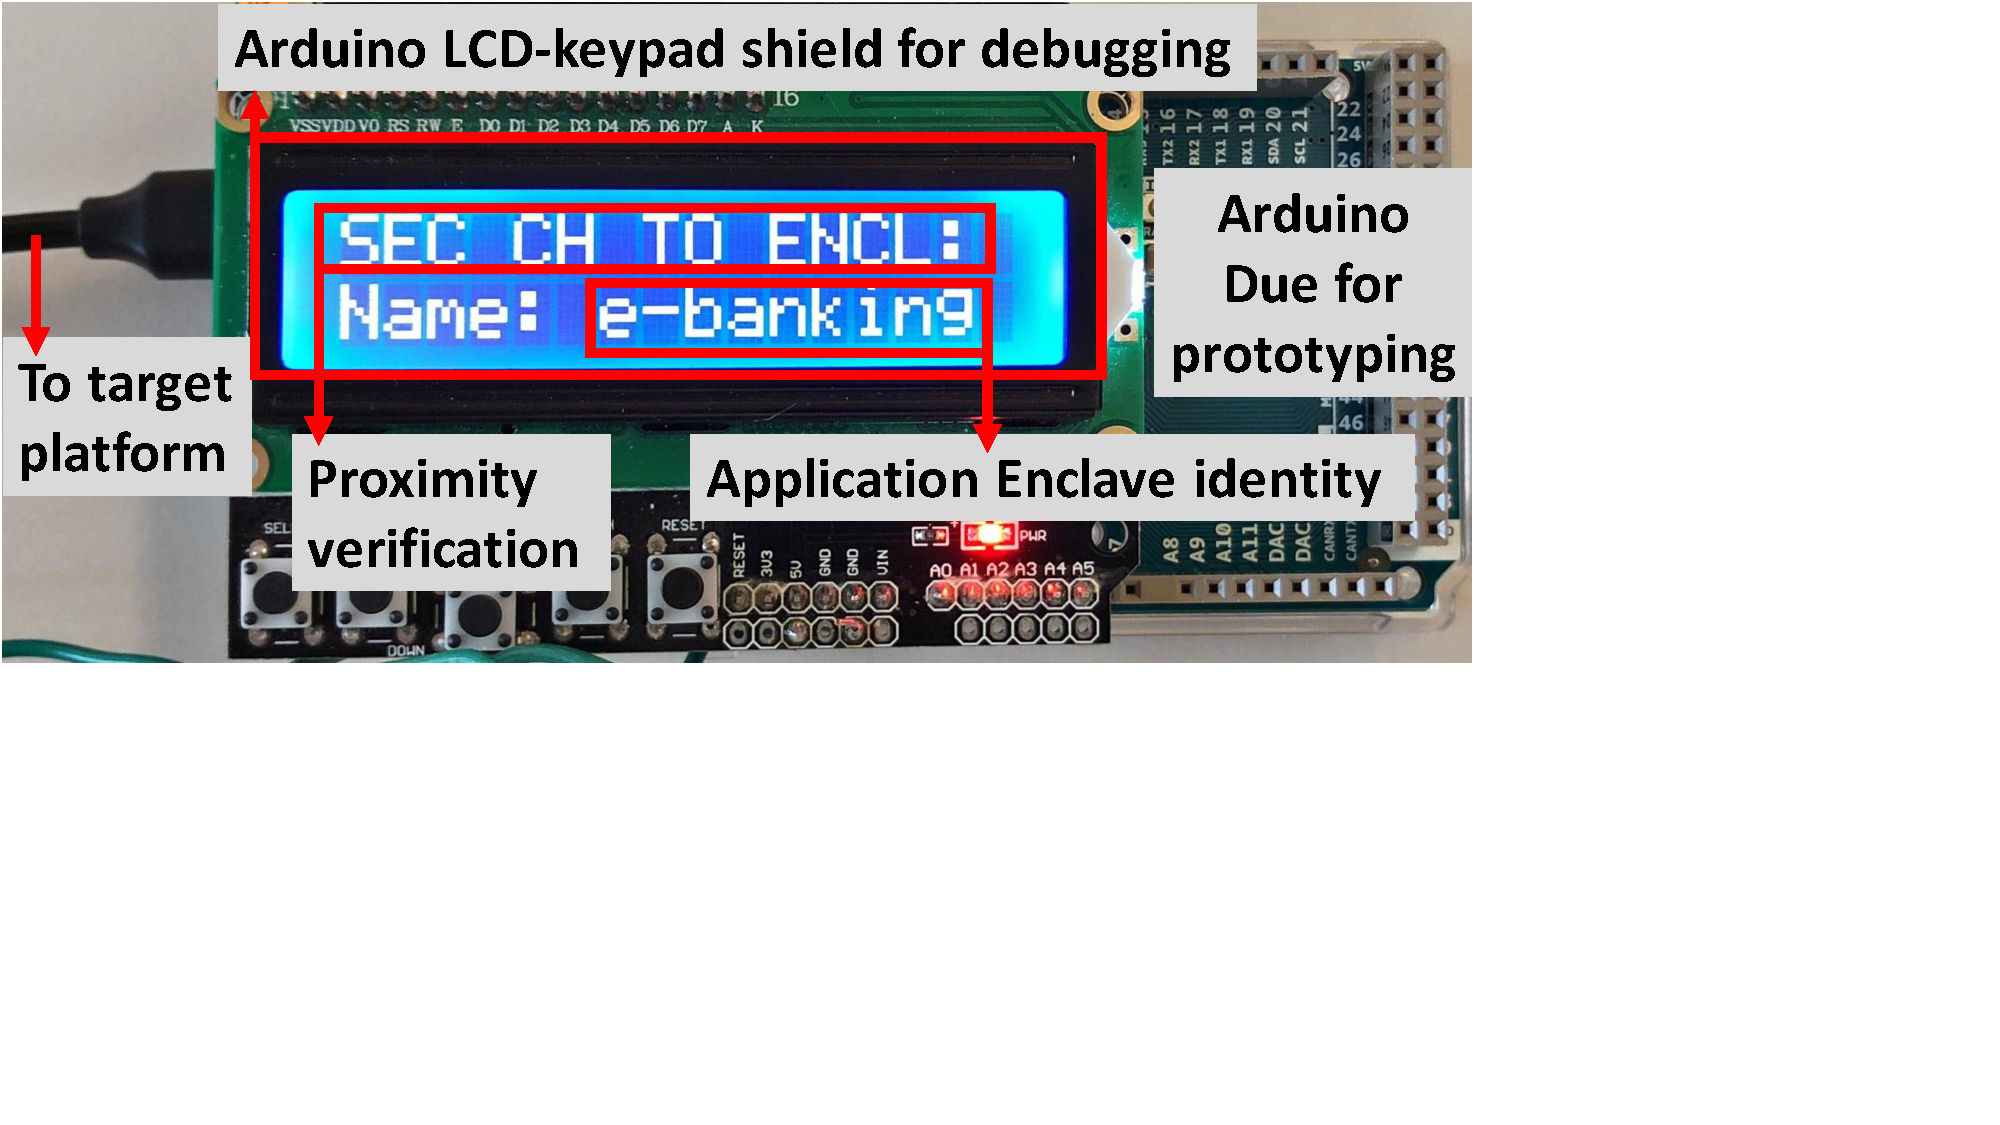
\includegraphics[trim={0 7.5cm 9cm 0}, clip, width=0.7\linewidth]{Setup1.pdf}
    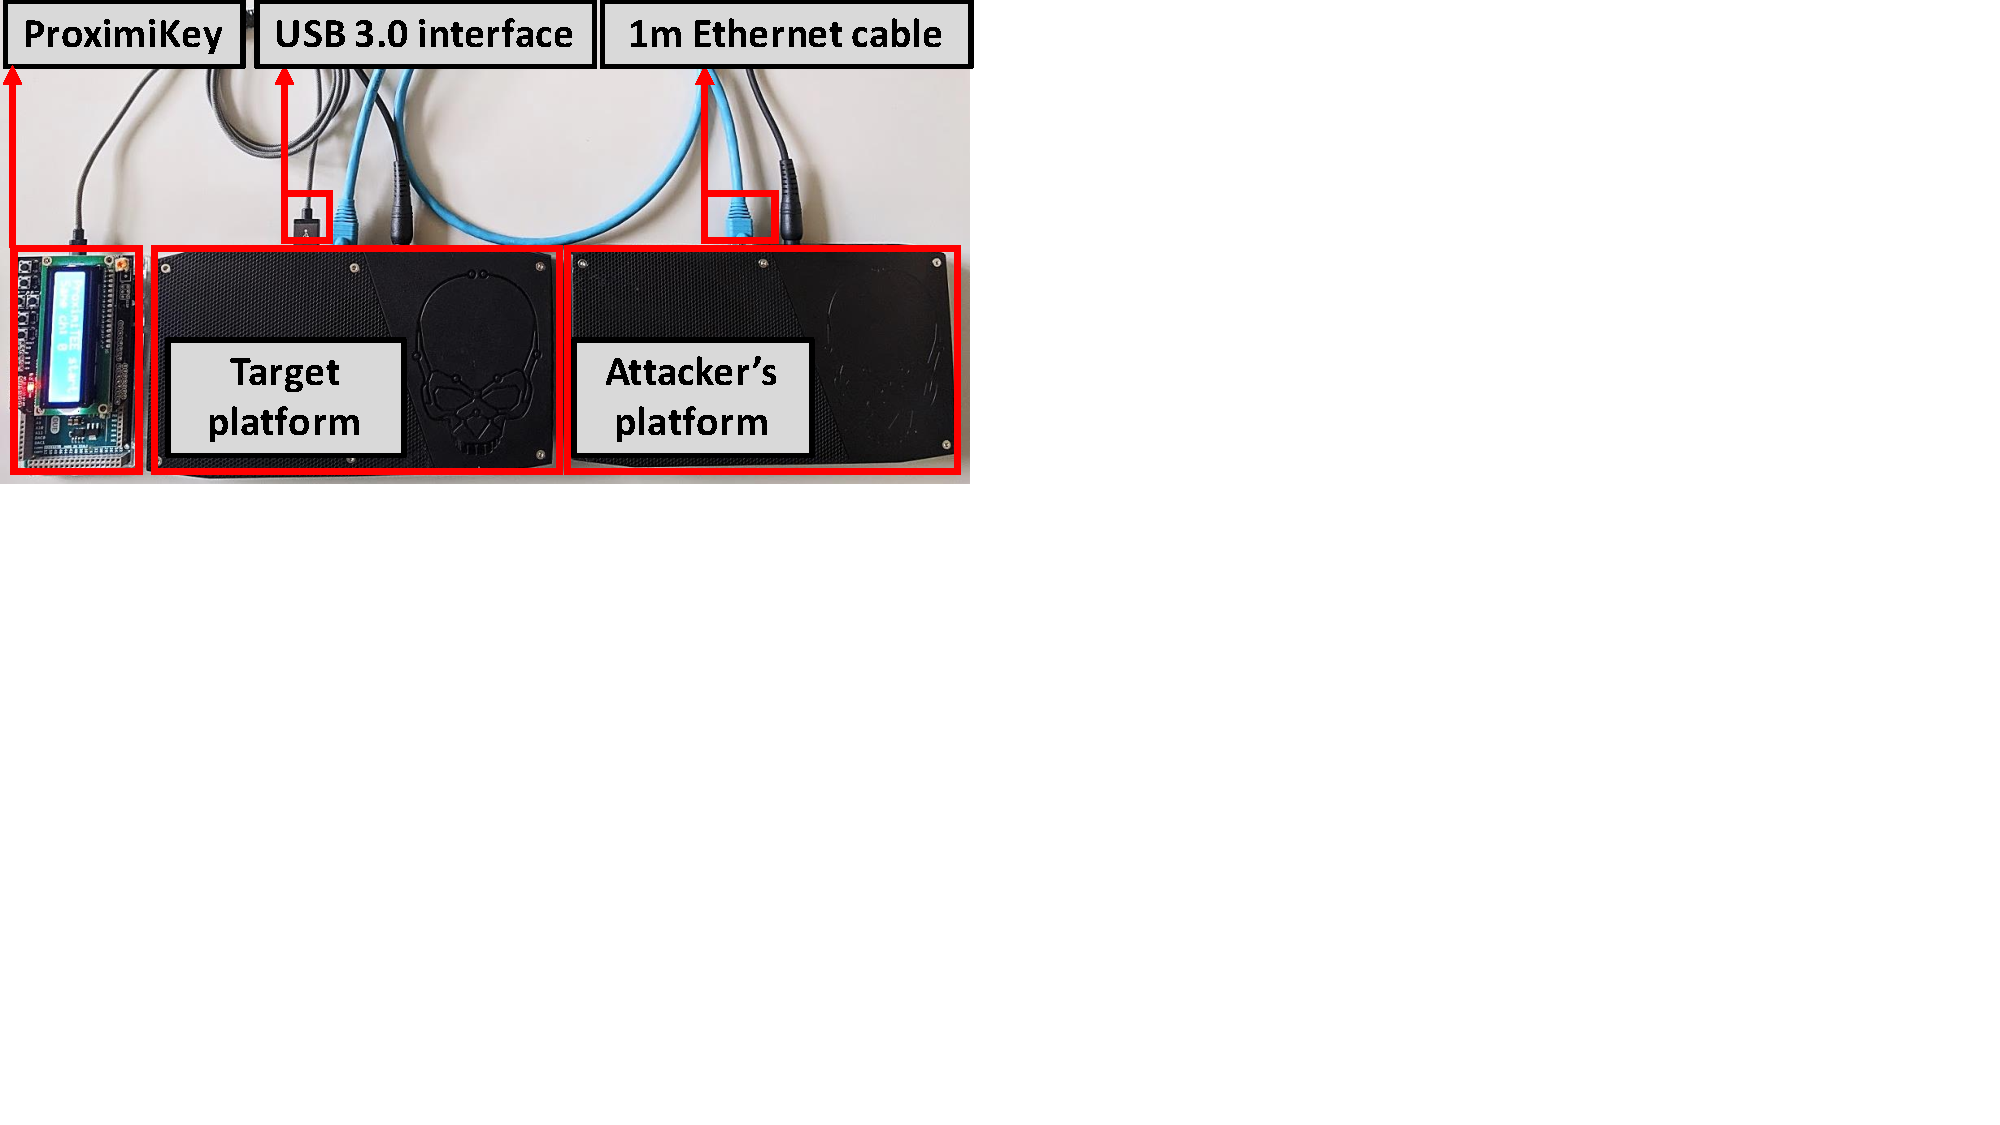
\includegraphics[trim={0 11cm 17cm 0}, clip, width=0.7\linewidth]{Setup2.pdf}
    \caption{\textbf{Test setup.} Our test setup consists of the \device device prototype, the target platform, the attacker's platform and the connection interfaces between them.}
   \vspace{-15px}
    \label{fig:setup}
\end{figure}

\section{Evaluation}
\label{sec:evaluation}

In this section, we describe our prototype implementation and experimental evaluation. In particular, we find suitable parameters for secure, reliable and fast proximity verification.

\subsection{Implementation}
\label{sec:evaluation:implementation}

We implemented a complete prototype of the \name system. Our implementation consists of three components: (i) \device prototype, (ii) \name enclave API which enables any \app to communicate with the \device device and execute our protocols, and (iii) \name kernel prototype.

\ifusenix
\vspace{-12pt}
\else
\fi
\myparagraph{\device.} Our \device prototype consists of one Arduino Due prototyping board equipped with an $84$ MHz ARM Cortex-M3 microcontroller. %, as shown in Figure~\ref{fig:setup}. 
The board communicated with the target platform over native \usb 2.0 connection that provides high-speed 480 Mbps connection.%\footnote{According to the \usb specification~\cite{usb20spec}, the speed between the host and the \usb device is negotiated dynamically.}.
%
We use the Arduino cryptographic library~\cite{ardCrypto} for the \tls. The limited set of cipher suites in our implementation uses $128$-bit AES (CTR mode) for encryption, AES-HMAC for message authentication code,  Curve25519 for Diffie-Hellman for key exchange and SHA256 for the hash function.
\iffalse
There are two ways an Arduino Due board can be connected to a host system: i) by the programming port which is serial over the \usb connection, and ii) the native \usb port where the Due acts as a native \usb device. The \usb over serial relays all the communication packets via the UART chip which has around 1 ms delay and achieves the maximum of $115200$ baud per second throughput. We opted for the native \usb port as it uses faster \usb 2.0 decoder and can achieve significantly better speed (according to the \usb specification, the speed between the host and the device is negotiated dynamically).
\fi
Our prototype implementation is approximately $200$ lines of code, and the code size of the \tls library is around $3.6$ KLoC.




%We used native Arduino \texttt{micros()} function to estimate the proximity latency in microsecond resolution. \todo{Move later, this is about experiments, not implementation}

\ifusenix
\vspace{-12pt}
\else
\fi
\myparagraph{\name kernel.} We have modified an image of Tiny Core Linux~\cite{tinyCore}, and used it as the boot image for our attestation variant II (cf.\ Section~\ref{sec:variantII}). The image size of our modified Linux distribution is 14 MB (in contrast to 2 GB standard 64 bit Linux images build on the standard kernel). Our image supports bare minimum functionality and includes \texttt{libusb}, \texttt{gcc}, Intel SGX SDK, Intel SGX platform software (PSW), and Intel SGX Linux driver.

\ifusenix
\vspace{-12pt}
\else
\fi
\myparagraph{\name enclave API.} The \name API for \app{}s is written in C++ using the Intel SGX API. The API uses native SGX crypto library for \tls implementation. The prototype is around 200 lines of code.


\iffalse
\subsection{Distance-Bounding Evaluation Approach}

\begin{figure}[t]
 \centering
  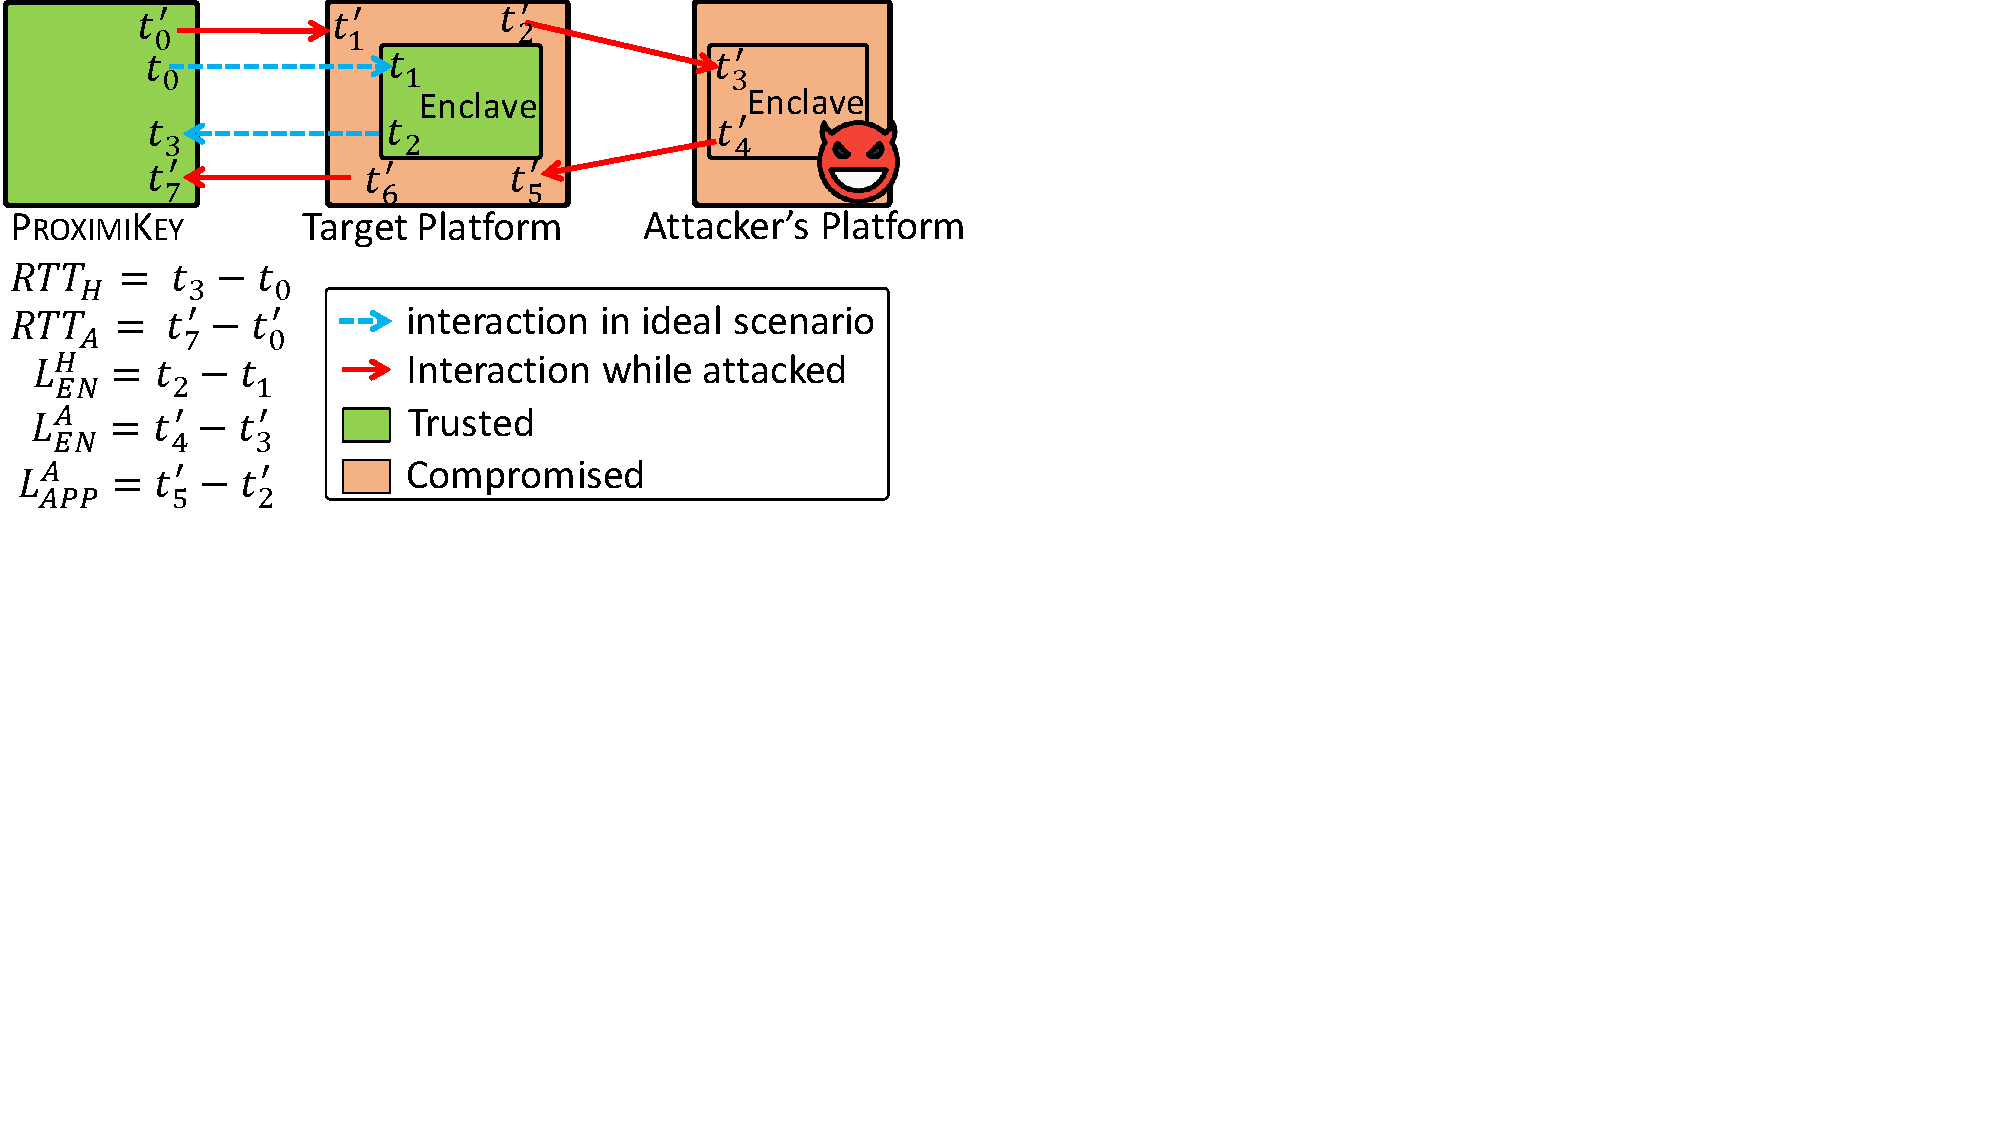
\includegraphics[trim={0 10.4cm 17cm 0},clip,width=0.84\linewidth]{TimeLine_revised.pdf}
 \caption{\textbf{Latencies and round trip times.} Blue dotted line illustrates normal attestation and red solid line illustrates relay attack.}
 \vspace{-2.3em}
 \label{fig:latency}
\end{figure}

To evaluate our proximity verification, we simulate an adversary that has the unlimited computing power and is connected to the target platform over a high-speed network connection.
Figure~\ref{fig:latency} illustrates round-trip times and computational latencies corresponding to benign proximity verification (dotted line) and rerouting attack scenarios (solid line). In this figure, $L_{APP}^H=t_{2}^\prime-t_{1}^\prime$ denotes the computational latency on the target platform that TLS processing for the received challenge (decryption), challenge increment and TLS processing for the sent response (encryption). $L_{APP}^A=t_{5}^\prime-t_{2}^\prime$ denotes the adversary's latency of rerouting the attestation challenge to the remote attacker's platform and back. And finally, $L_{EN}^A=t_{4}^\prime-t_{3}^\prime$ denotes the adversary's computational latency for similar operation.

Since the adversary might have a faster processor than the one of the target platform, we simulate the worst case scenario, where the adversary's computation happens instantly, i.e., we set $L_{EN}^A=0$ ($t_{3}^\prime=t_{4}^\prime$).
%
Thus, the difference of latency in the normal and the relayed challenge-response merely is the round-trip time to the adversary's platform and back ($L_{APP}^A$).
\fi

\ifusenix
\subsection{Experimental Setup}
\else
\subsection{Experimental Setup and Simulated Relay Attack}
\fi
\label{sec:evaluation:exp}

We conducted our experiments on three SGX platforms: two Intel NUC NUC6i7KYK mini-PCs and one Dell Latitude laptop, all equipped with SGX-enabled Skylake core i7 processors and Ubuntu 16.04 LTS installed on them.

We performed two types of experiments. First, we tested legitimate attestation of an enclave on the target platform (i.e., SGX platform to which our \device prototype was connected to). Second, we \emph{simulated} a relay-attack adversary whose platform was connected to the target platform via a direct Ethernet cable (see Figure~\ref{fig:setup}). Since the adversary might have a faster processor than the one of the target platform, we simulate the worst case scenario, where the adversary's computation needed for the proximity verification protocol happens instantly. Instant replies were simulated by fixing the randomness for the challenges and having precomputed responses for that randomness on the attacker's machine. 


For the relay-attack, we tested three different Ethernet cables of length 1m, 7m and 10m to evaluate the effect on the latency. For the legitimate proximity verification, we used a standard \usb cable of length 1m and a \usb extender cable or length 2m to evaluate the effect of \usb cable length on the latency. We also tested two different SGX platforms and two different embedded device prototypes.

We experimented with the achievable round-trip time between the target and the simulated attacker's platform. First, we tested the standard \texttt{ping} tool which gave a latency of around $380\ \mu s$ for one-meter Ethernet connection. After that, we used \texttt{ping} tool in so called flood mode~\cite{ping} and measured a reduced average network latency of around $153\ \mu s$ (command \texttt{ping -s 300 -af}). The used flood mode achieves faster round-trip time as the it forces the OS to fill up the network queue of the kernel. As our adversary fully controls the OS, we chose to simulate an attacker that fills the kernel's network queues similar to the flood mode to minimize latency.

To measure latencies we used Arduino's native \texttt{micros()} that provides (10s of) microsecond level accuracy. To achieve more accurate time measurements, we also used a high precision 8 Ghz Keysight Infinium oscilloscope. We performed a total of $27.8$ million rounds of the protocol for normal attestations and $15$ million rounds for simulated attacks and measured the challenge-response latencies for each. We measure all of them inside the Arduino code. For cross-validation, we tested the \device with the high precision oscilloscope and witnessed identical timing patterns.

\ifusenix
\vspace{-5pt}
\else
\fi
\subsection{Main Experimental Result}
\label{sec:evaluation:results}


\begin{figure}[t]
  \centering
    %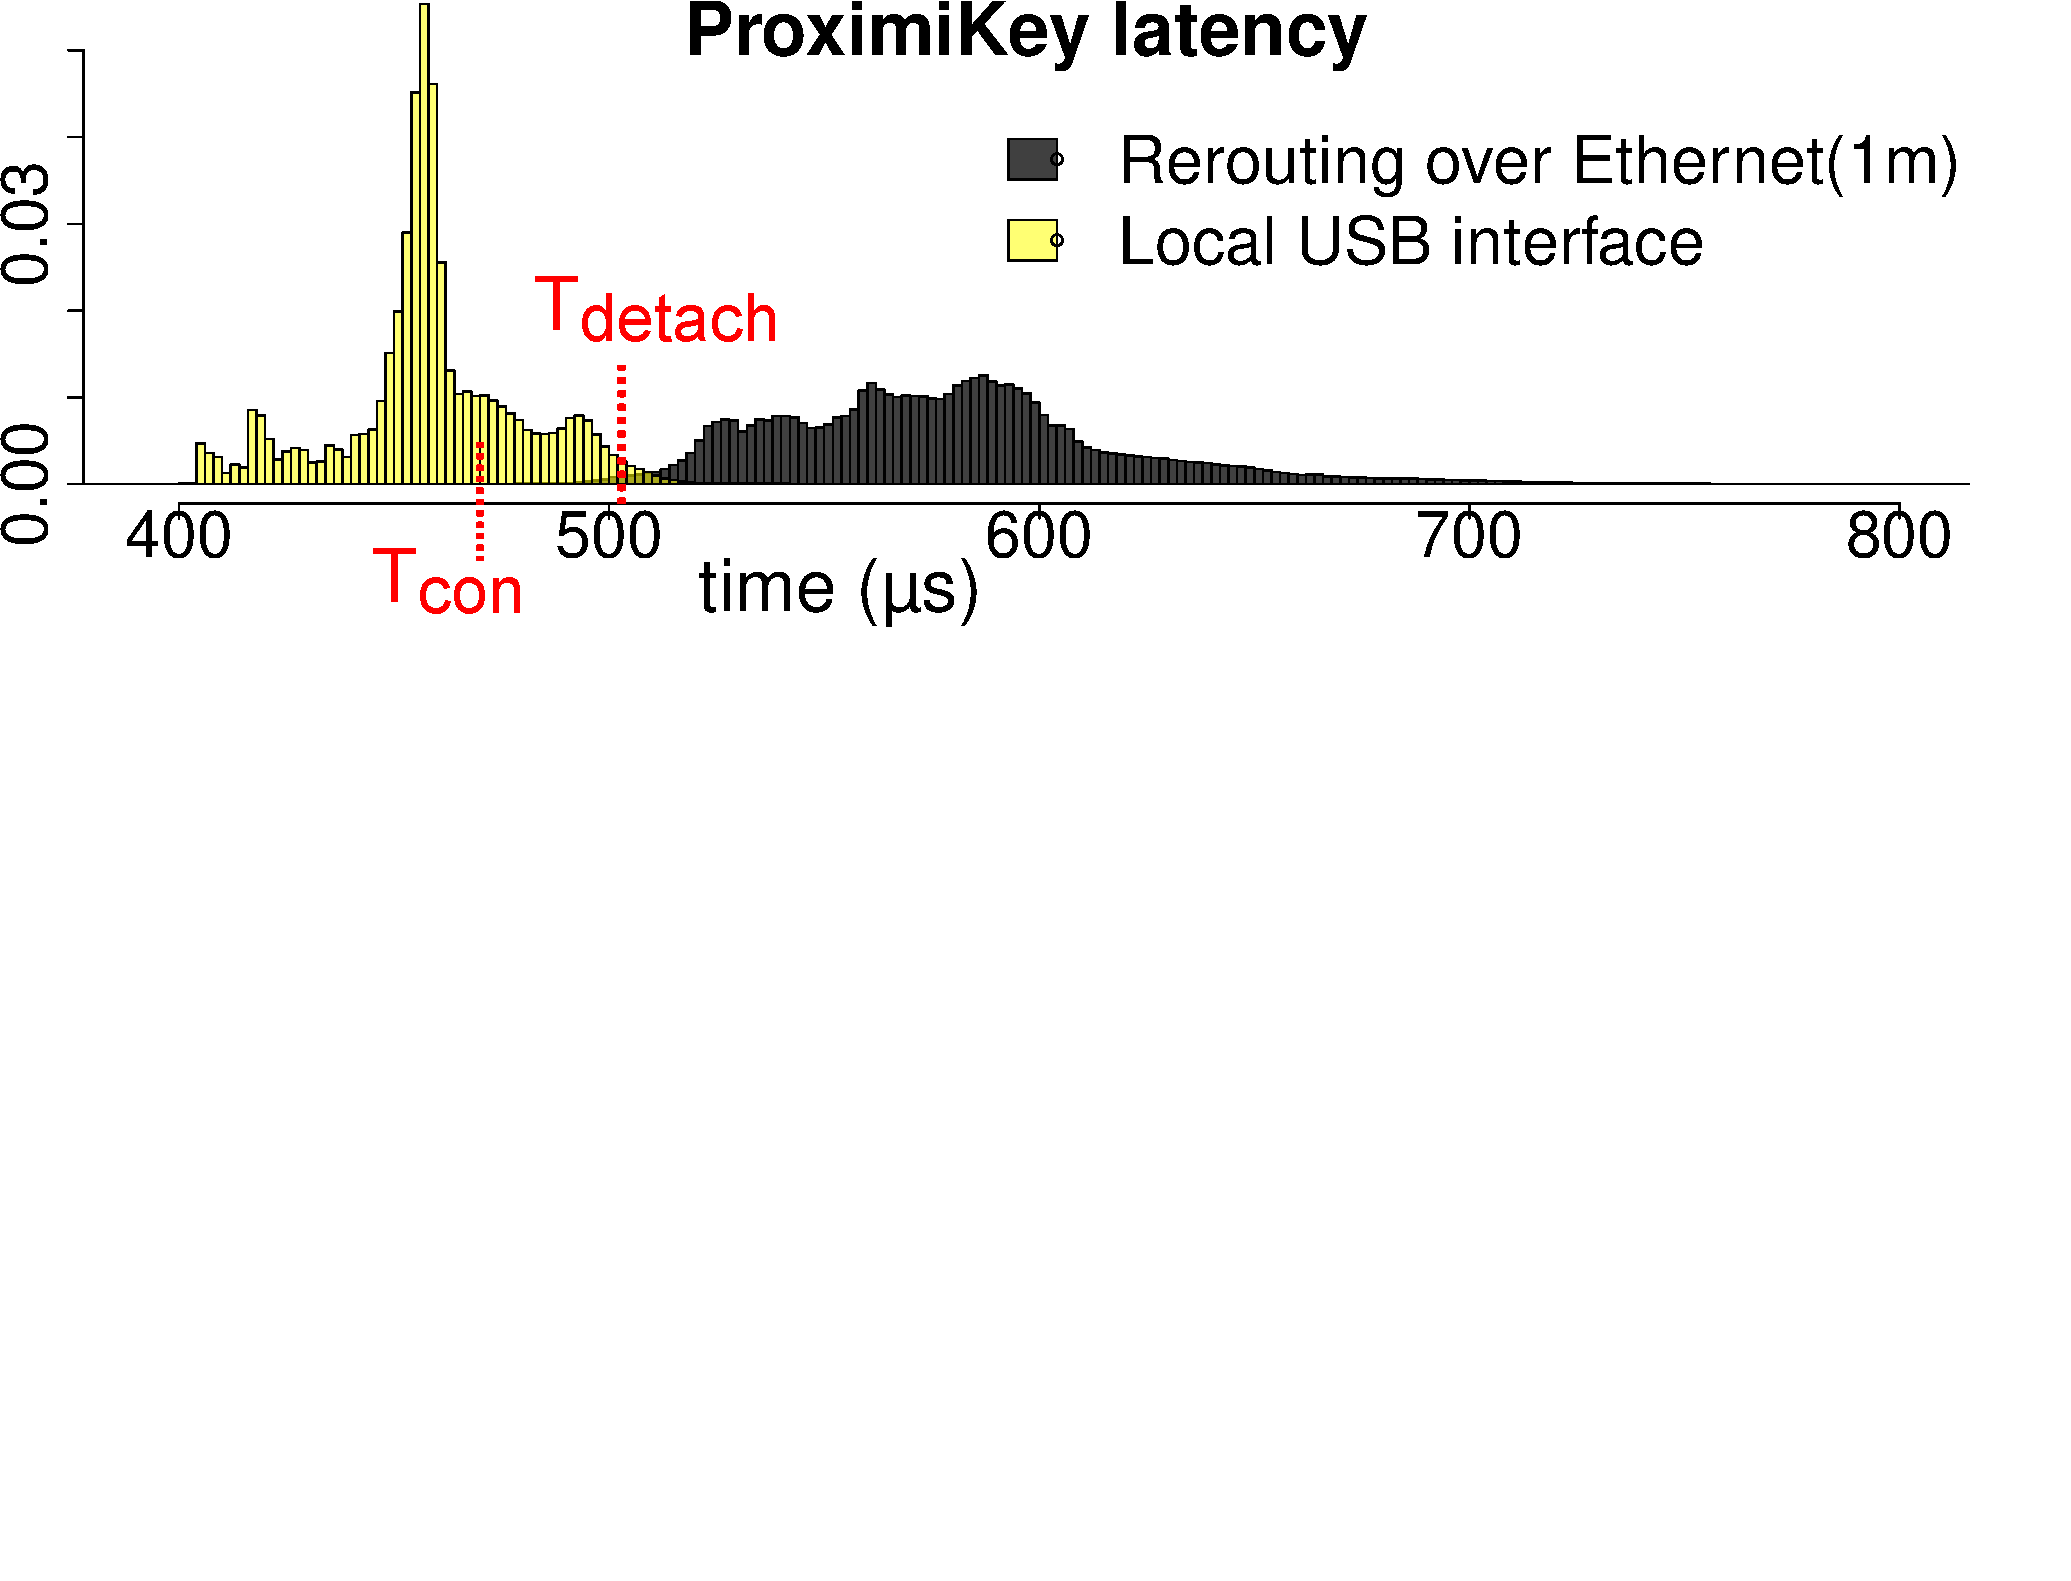
\includegraphics[trim={0 3cm 0.5cm 0}, clip, width=\linewidth]{data/graph/Local_vs_Remote_Combined.pdf}
    %\includegraphics[trim={0 20cm 0.5cm 0}, clip, width=\linewidth]{data/graph/Local_vs_Remote_Combined_1.pdf}
    \ifusenix
    %\includegraphics[trim={0 19cm 3.5cm 0}, clip, width=0.9\linewidth]{data/graph/Local_vs_Remote_Combined_2.pdf}
    \includegraphics[trim={0 16.2cm 2cm 0}, clip, width=0.85\linewidth]{data/graph/Local_vs_Remote_Combined_new.pdf}
    \else
    %\includegraphics[trim={0 19cm 3.5cm 0}, clip, width=0.65\linewidth]{data/graph/Local_vs_Remote_Combined_2.pdf}
    \includegraphics[trim={0 16cm 2cm 0}, clip, width=0.65\linewidth]{data/graph/Local_vs_Remote_Combined_new.pdf}
    \fi
    \caption{\textbf{Challenge-response latency.} Latency frequency distributions when \device prototype is connected to the target platform over the \usb interface and for the simulated relay attack over a short Ethernet connection. \connect and \detach thresholds are placed at $470\ \mu s$ and $510\ \mu s$, respectively.}
    \vspace{-10pt}
    \label{graph:reroutingDetectionHist}
\end{figure}



Figure~\ref{graph:reroutingDetectionHist} shows our main experimental result for the 1 meter Ethernet and 1 meter USB cables case. The left histogram represents challenge-response latencies in the benign case, and the right histogram represents the latencies in the simulated attack. As can be seen from the figure, the vast majority of benign round-trips take from 394 to 647 $\mu s$ (average is 459 $\mu s$, $95\%$ samples are in between 400 $\mu s$ and 497 $\mu s$). The vast majority of the round-trip times in the simulated attack take from 451 to 1251 $\mu s$ (average is $579\ \mu s$, $95\%$ samples are in between $490\ \mu s$ and $655\ \mu s$).
%
The difference between the averages of the benign and attack scenarios is $120\ \mu s$ which is less than the previously tested flood mode \texttt{ping} latency ($153\ \mu s$). 

We report additional experiment results including the effects of different Ethernet and \usb cable lengths, different SGX platforms, and different \device{} prototypes in Appendix~\ref{appendix:ex}.

\subsection{Initial Proximity Verification Parameters}
\label{sec:evaluation:parameters}

In Section~\ref{sec:systemDesign} we explained that the initial proximity verification is successful when at least fraction $k$ of the $n$ challenge-response latencies are below the threshold \connect.  Now, we explain how to set these parameters based on the above experimental results.

In our solution, there are five interlinked parameters that one needs to consider: (i) the legitimate connection latency threshold \connect, (ii) total number of challenge-response rounds $n$, (iii) the fraction $k$, (iv) attacker's success probability $P_{adv}$ that should be negligible, and (v) the legitimate success probability $P_{legit}$ that should be high. We find suitable values for these parameters in the following order:


\begin{figure}[t]
  \centering
    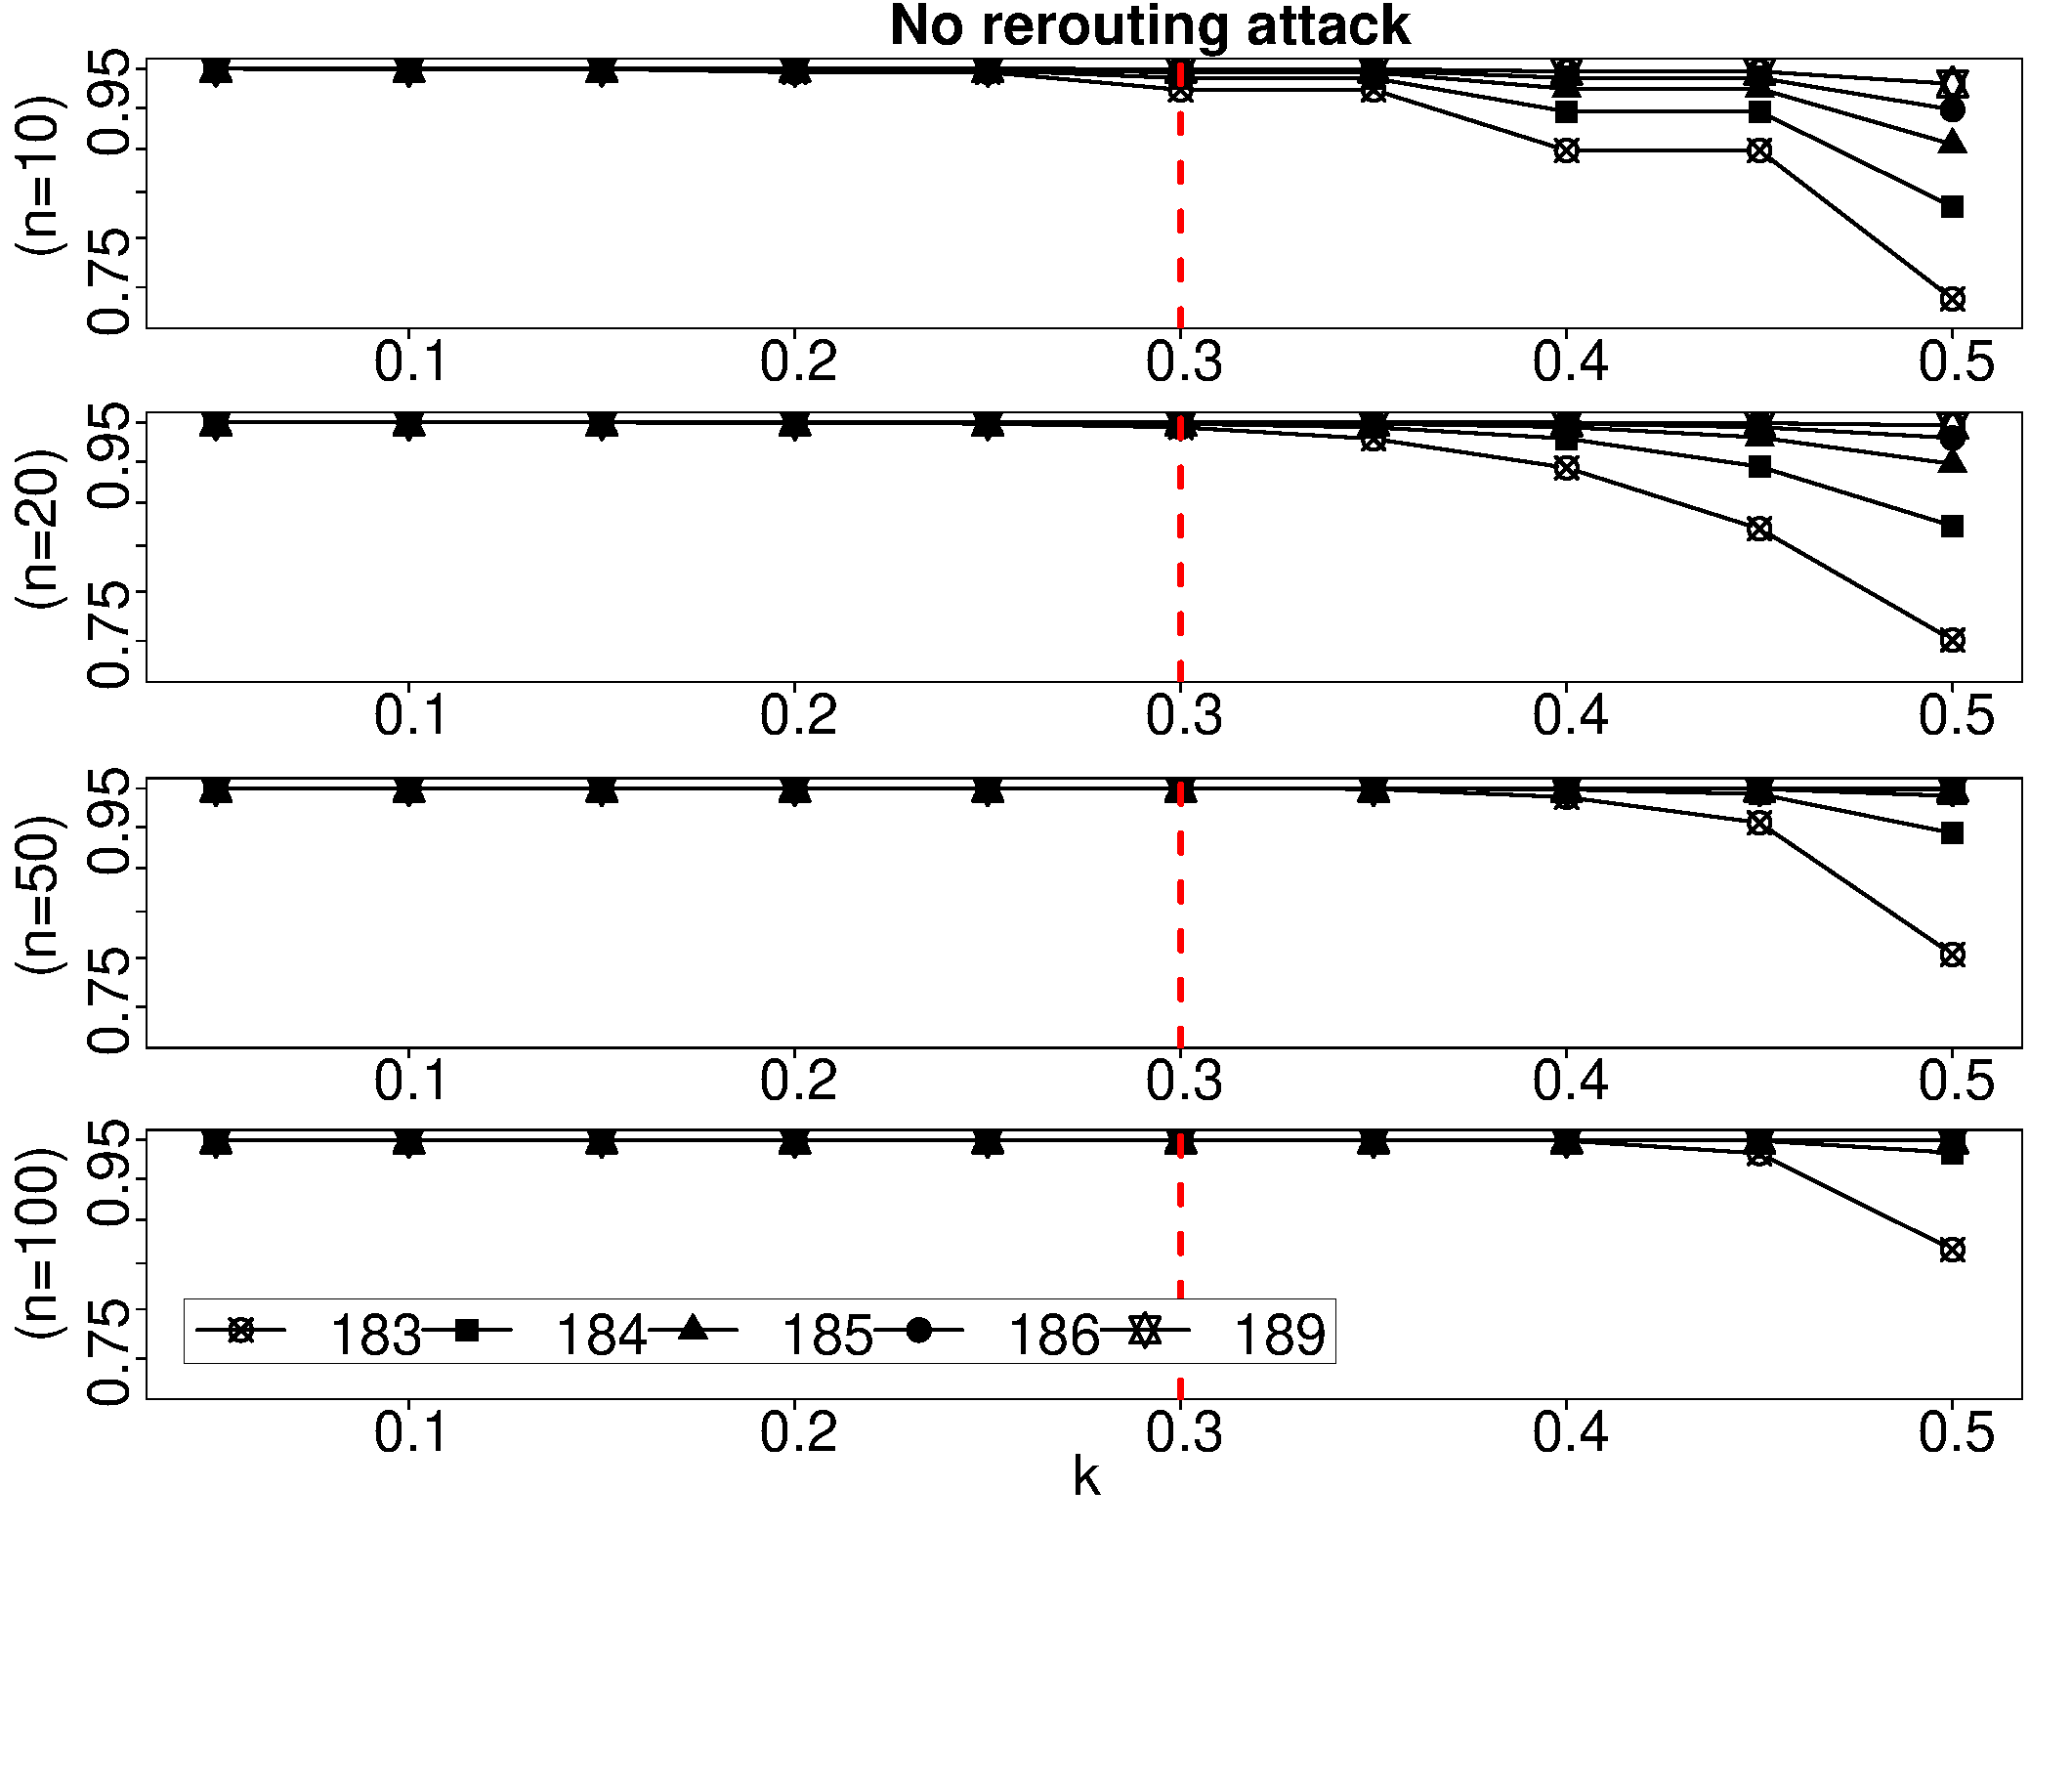
\includegraphics[trim={0 5cm 0 0}, clip, width=\linewidth]{data/fx3_data/timeRound.pdf}
    \caption{Legitimate attestation success probability for different \connect values. The chosen value \connect $=186\ \mu s$ gives success probability $0.999999977$ for number of trials at least 15 out of $n=50$ rounds when $k=0.3$.}
	\figsaver
    \label{graph:diffTh}
\end{figure}


\begin{figure}[t]
  \centering
    %\includegraphics[trim={0 0 0 0}, clip, width=0.4\linewidth]{data/graph/CDF_Latency.pdf}
    %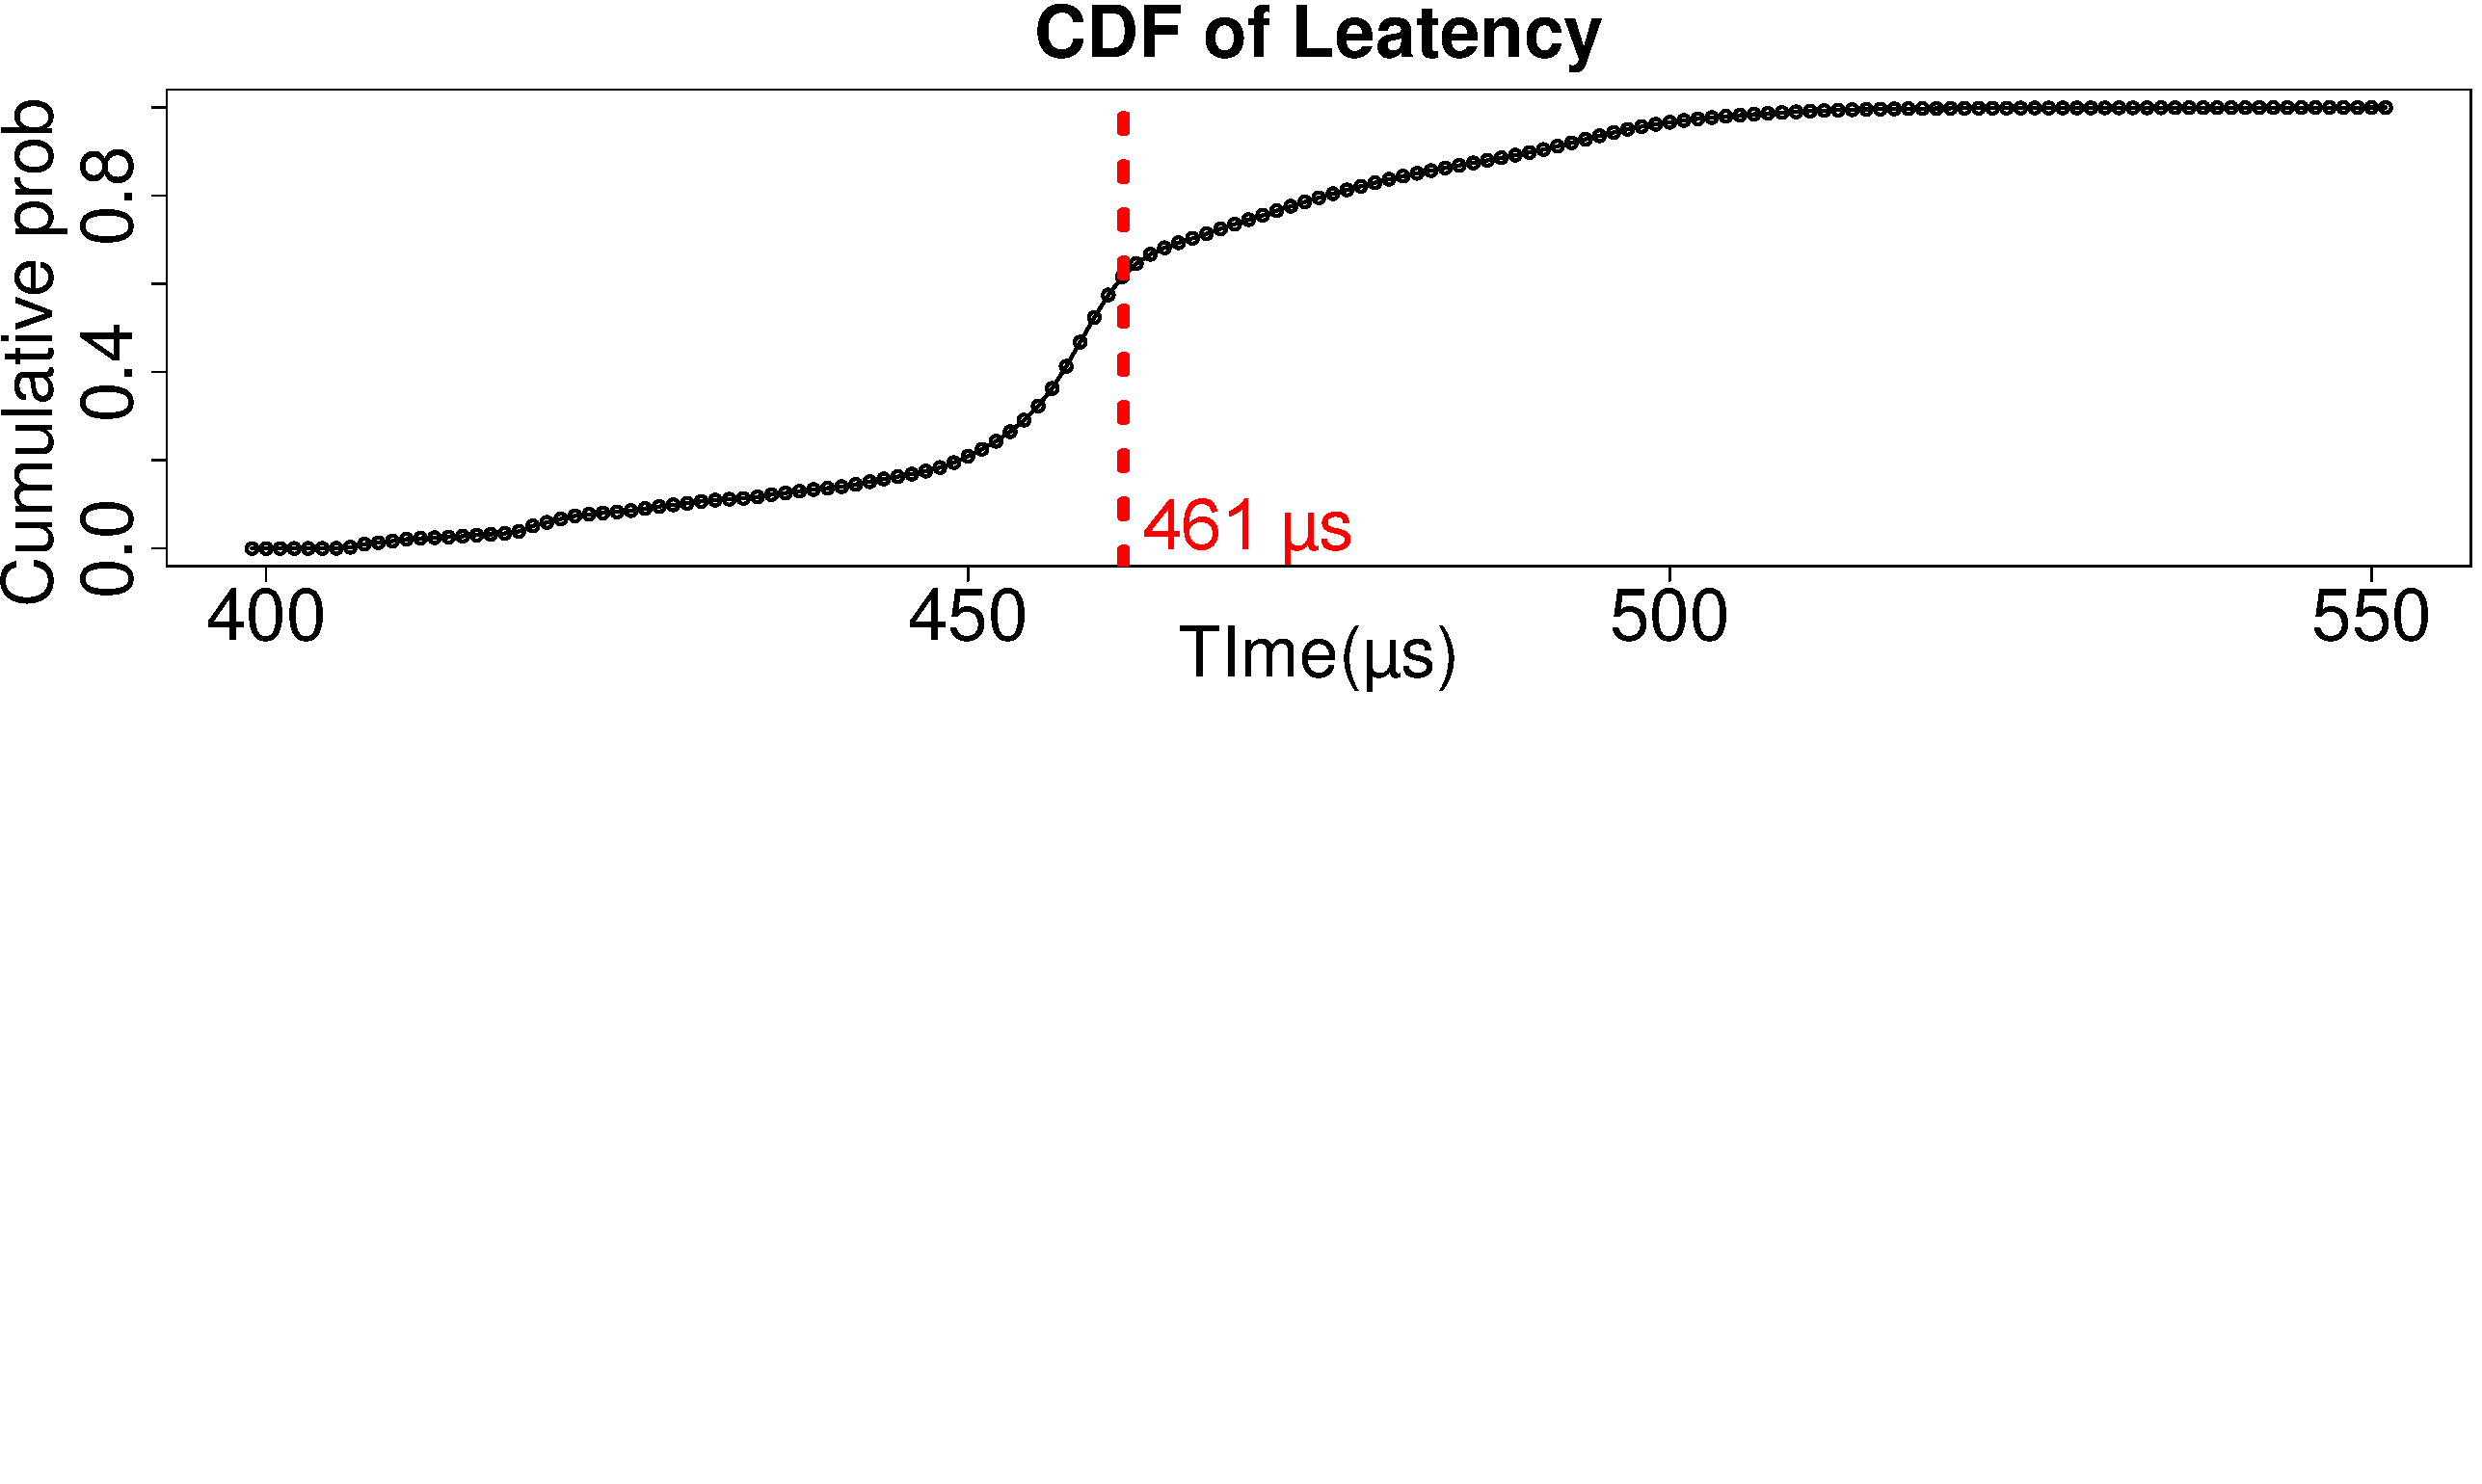
\includegraphics[trim={0 14cm 0 0}, clip, width=\linewidth]{data/graph/CDF_Latency1.pdf}
    %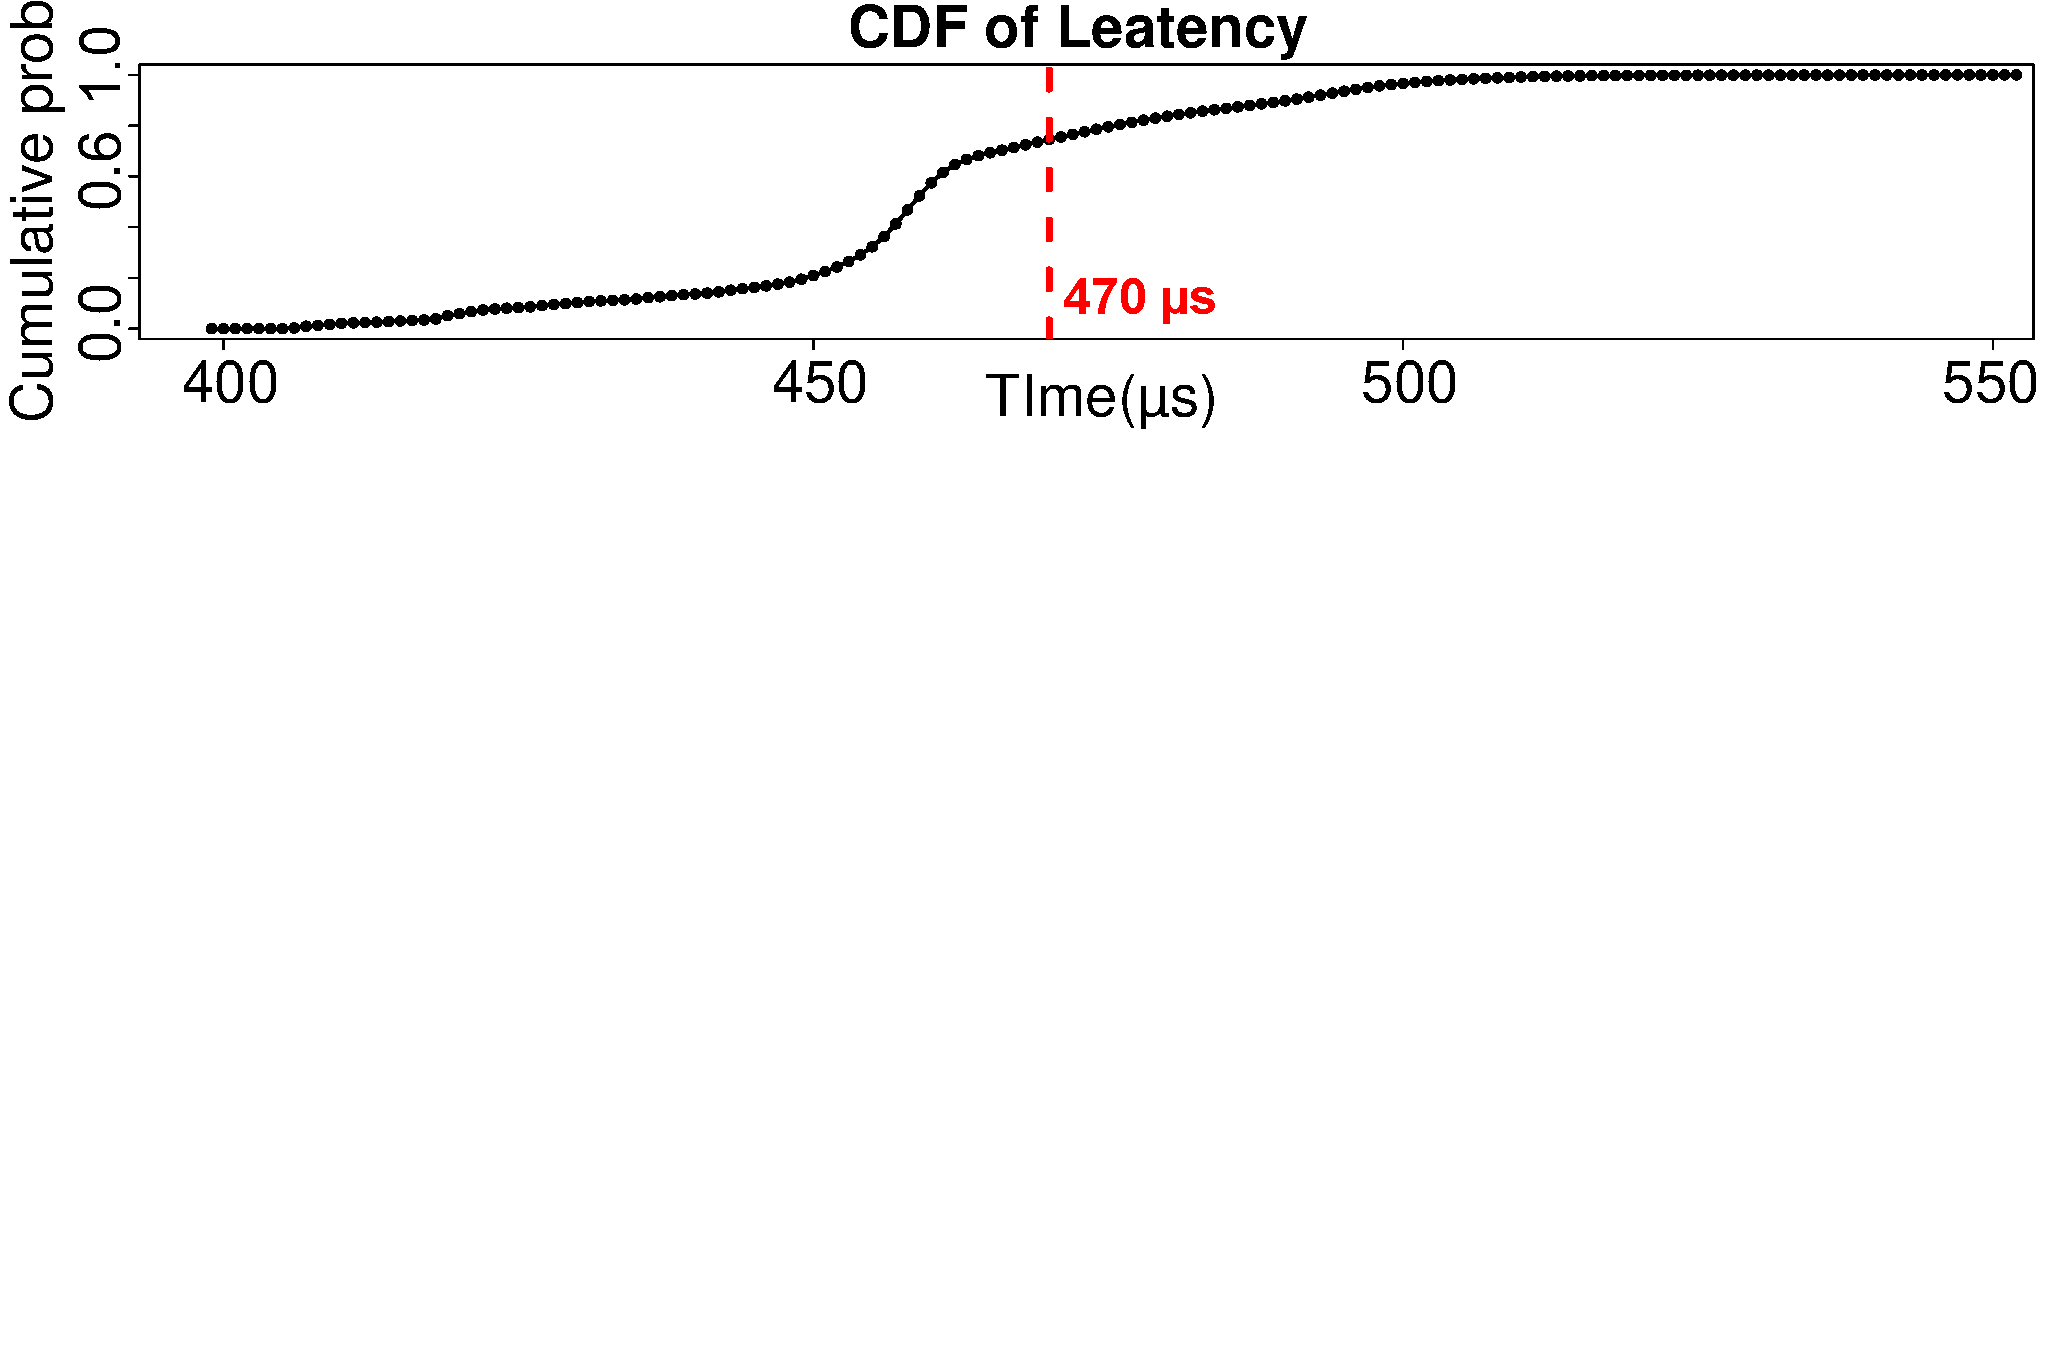
\includegraphics[trim={0 16cm 0 0}, clip,
    % width=\linewidth]{data/graph/CDF_Latency_new.pdf}
    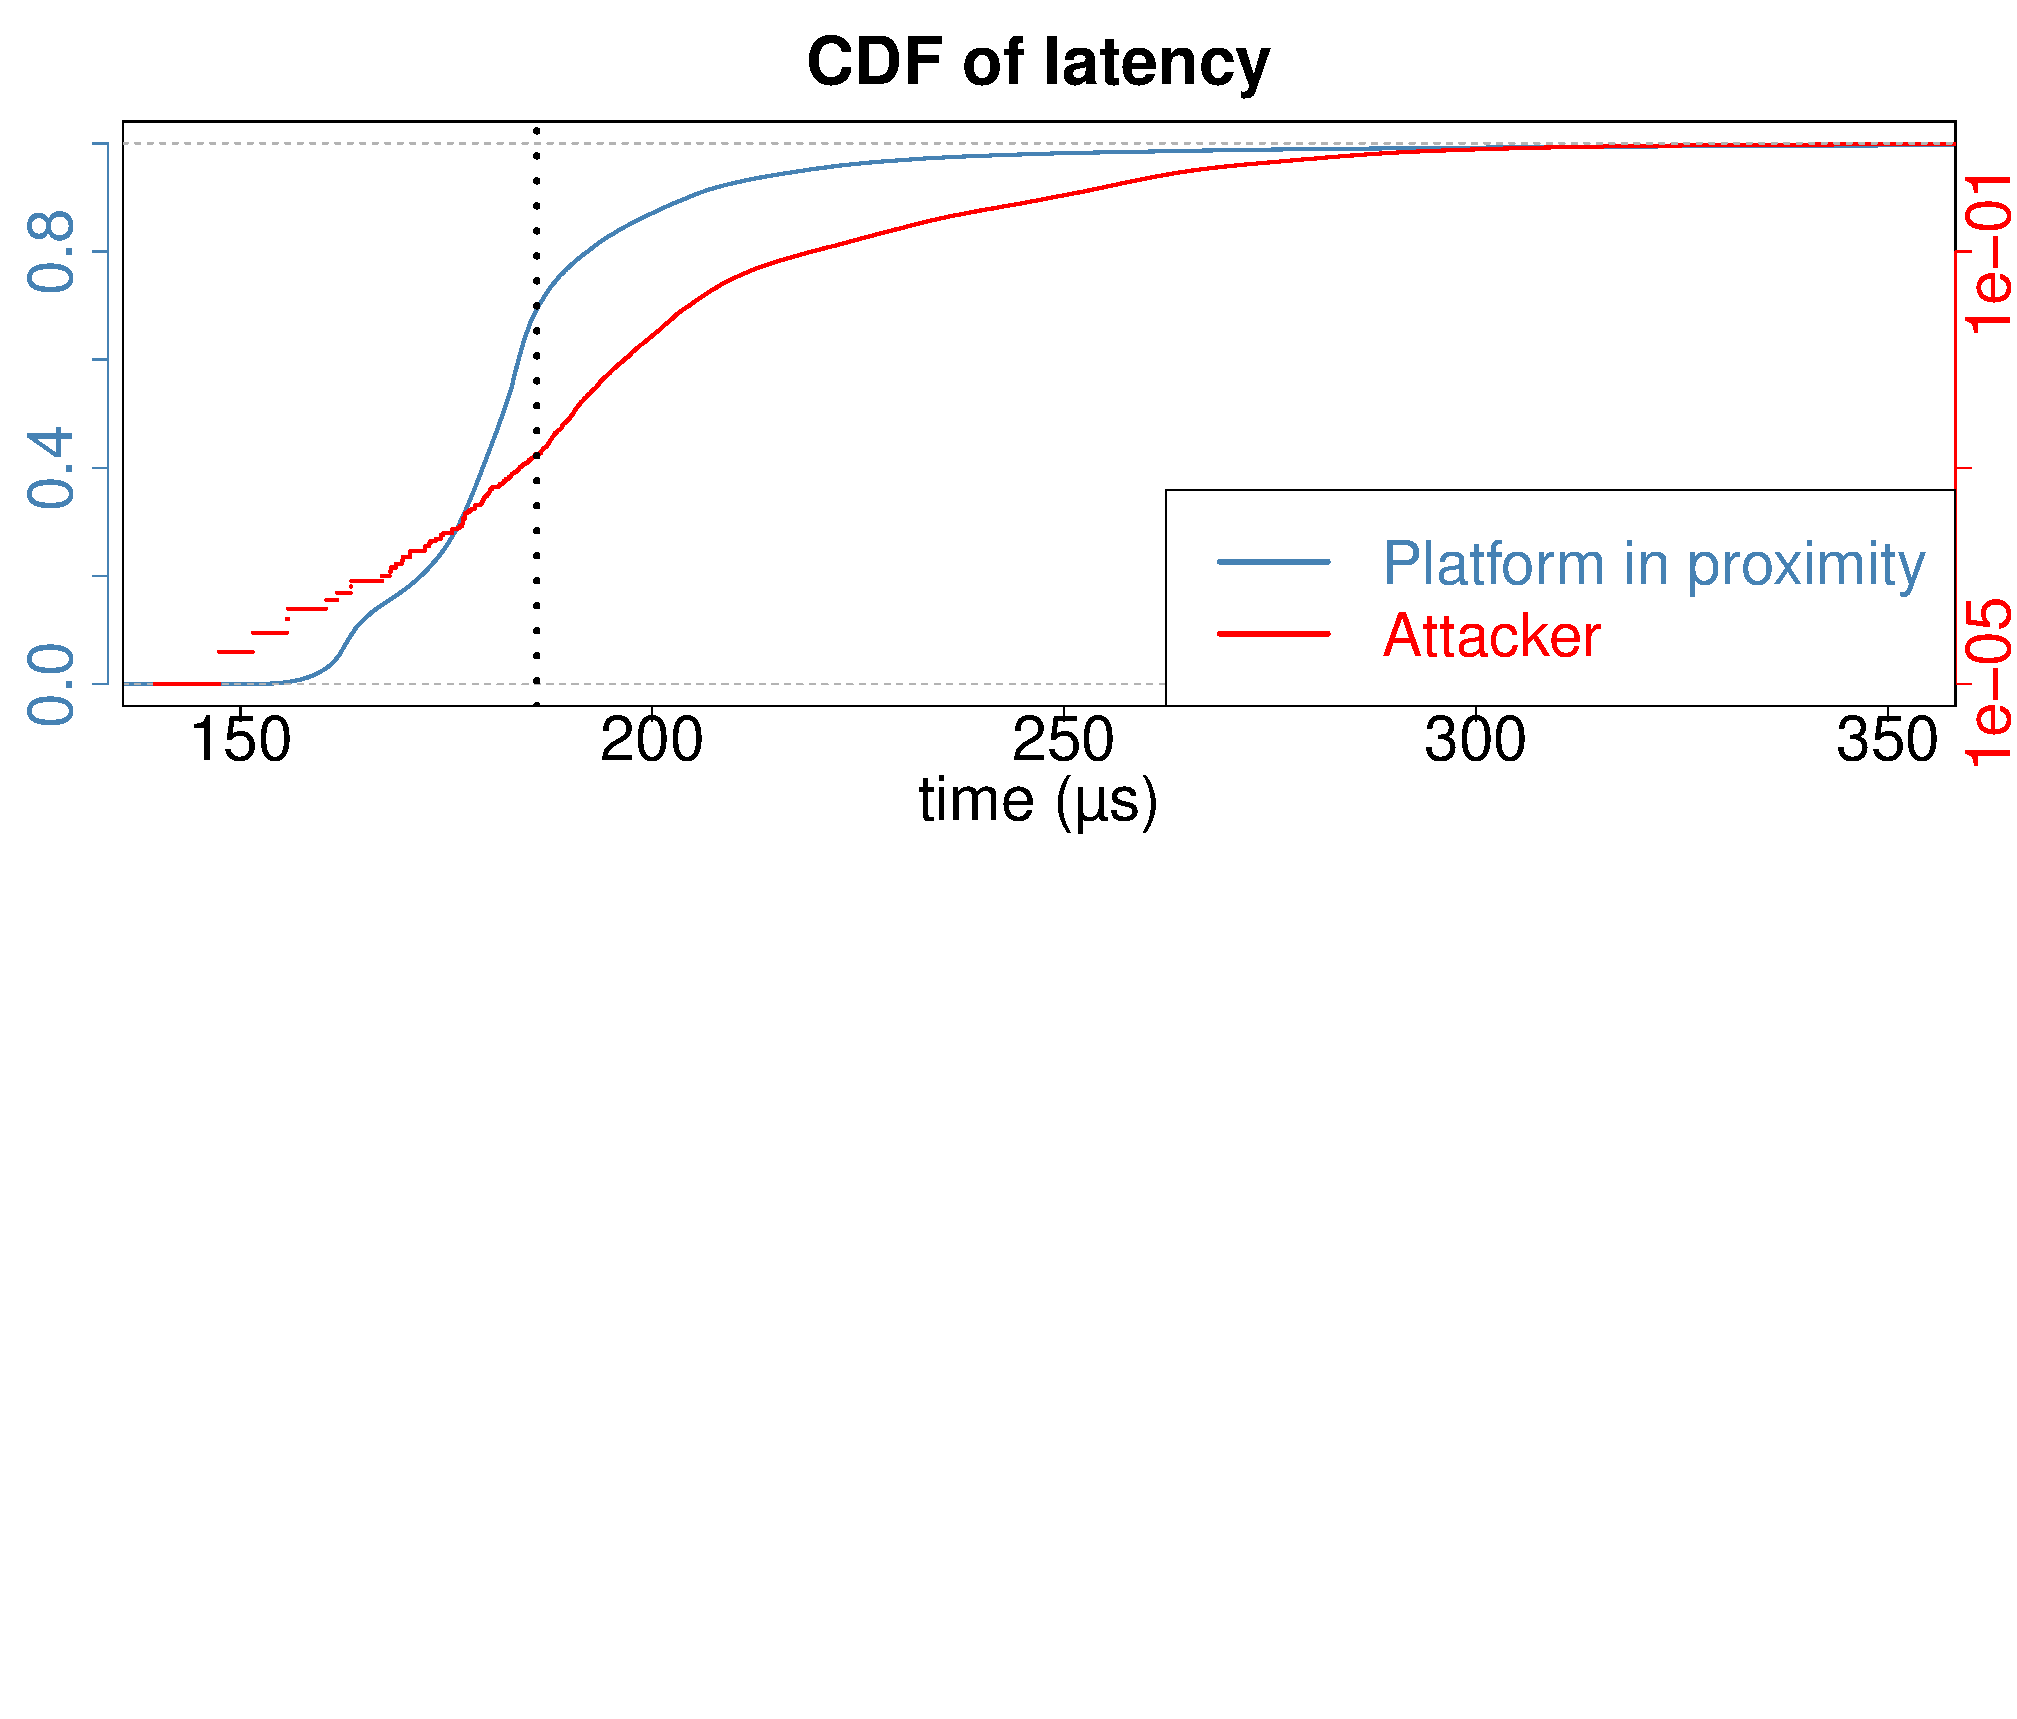
\includegraphics[trim={0 15cm 0 0}, clip, width=\linewidth]{data/fx3_data/CDF_N.pdf}
    \caption{Cumulative distribution function for latencies. We set the threshold \connect at 183 $\mu s$ which has a cumulative probability of $0.693$ in the experiment where no rerouting attack takes place with probability of $1.33\times10^{-4}$.}
    \vspace{-10pt}
    \label{fig:cdf}
\end{figure}


\myparagraph{1. Finding suitable threshold \connect.} Finding a suitable threshold \connect is a non-trivial task. A very low threshold requires a high number of the challenge-response rounds, since the protocol requires at least a fraction $k$ of the observed responses to be less or equal to \connect and a low threshold has very low cumulative probability value in the latency distribution (see Figure~\ref{fig:cdf}). Conversely, a very high threshold value enables some latencies measured during an attack to be classified as legitimate replies, hence increasing the chances of the attacker to break the proximity verification. To address this challenge, we perform a trial over multiple threshold candidates to evaluate their viability.


Figure~\ref{graph:diffTh} shows the legitimate success probability $P_{legit}$ for different number of rounds ($n\in\{10,20,50,100\}$). We iterate through multiple threshold times (\connect$\in\{183\mu s,184\mu s,185\mu s, 186\mu s, 189\mu s\}$), and $186\mu s$ provides high success ratio for different values of $k$ ($P_{legit}=0.9\{7\}77$ $(n=50)$ and $P_{legit}=0.9\{15\}29\ (n=100)$), where $0.9\{n\}x$ denotes $0.n$-times $9$ followed by $x$.

We test \connect up until $186 \mu s$ because as can be observed in Figure~\ref{graph:instatAttackerHisto} for these values we observe extremely small occurrences ($1.33\times10^{-3}$) of latency responses during an attacking scenario. It is possible to increment the latency further to improve the success probability, but doing so will start increasing the probability for the attacker as well. 
%
After that, we estimate that any latency value less than or equals to the threshold \connect appears with the cumulative probability of $p_{\mathcal{H}} = \Pr[144\leq x \leq 186] = \sum_{i=144}^{186}\Pr[x=i] = 0.693$ (where $144\ \mu s$ is the smallest latency experienced).

The attacker's success probability for a single round is the cumulative probability sampled from the attacker's distribution (the grey histogram in Figure~\ref{graph:instatAttackerHisto}) $p_\mathcal{A} = \Pr[x \leq 186] = \sum_{i=160}^{183}\Pr[x=i] = 1.33 \times 10^{-4}$.


Now, for both cases (simulated attack and benign case) we can model the complete challenge-response protocol of $n$ rounds as a Bernoulli's trial where we look for at least $kn$ responses within $186\ \mu s$ out of $n$. We can write this cumulative probability as a binomial distribution:
%

\begin{align*}
    \Pr[x \geq nk] = \sum_{i=nk}^n\binom{n}{i} (p)^{i}(1-p)^{n-i};~~\text{where}~ p \in \{p_\mathcal{H}, p_\mathcal{A}\}
\end{align*}
%  \vspace{-3px}


\newcommand{\roundCompCaption}{\textbf{Finding suitable fraction $k$.} The graph shows the legitimate enclave's success probability in an ideal scenario and the attacker's success probability in rerouting attack scenario with varying $k$.}

\begin{figure}[t]
  \centering
    %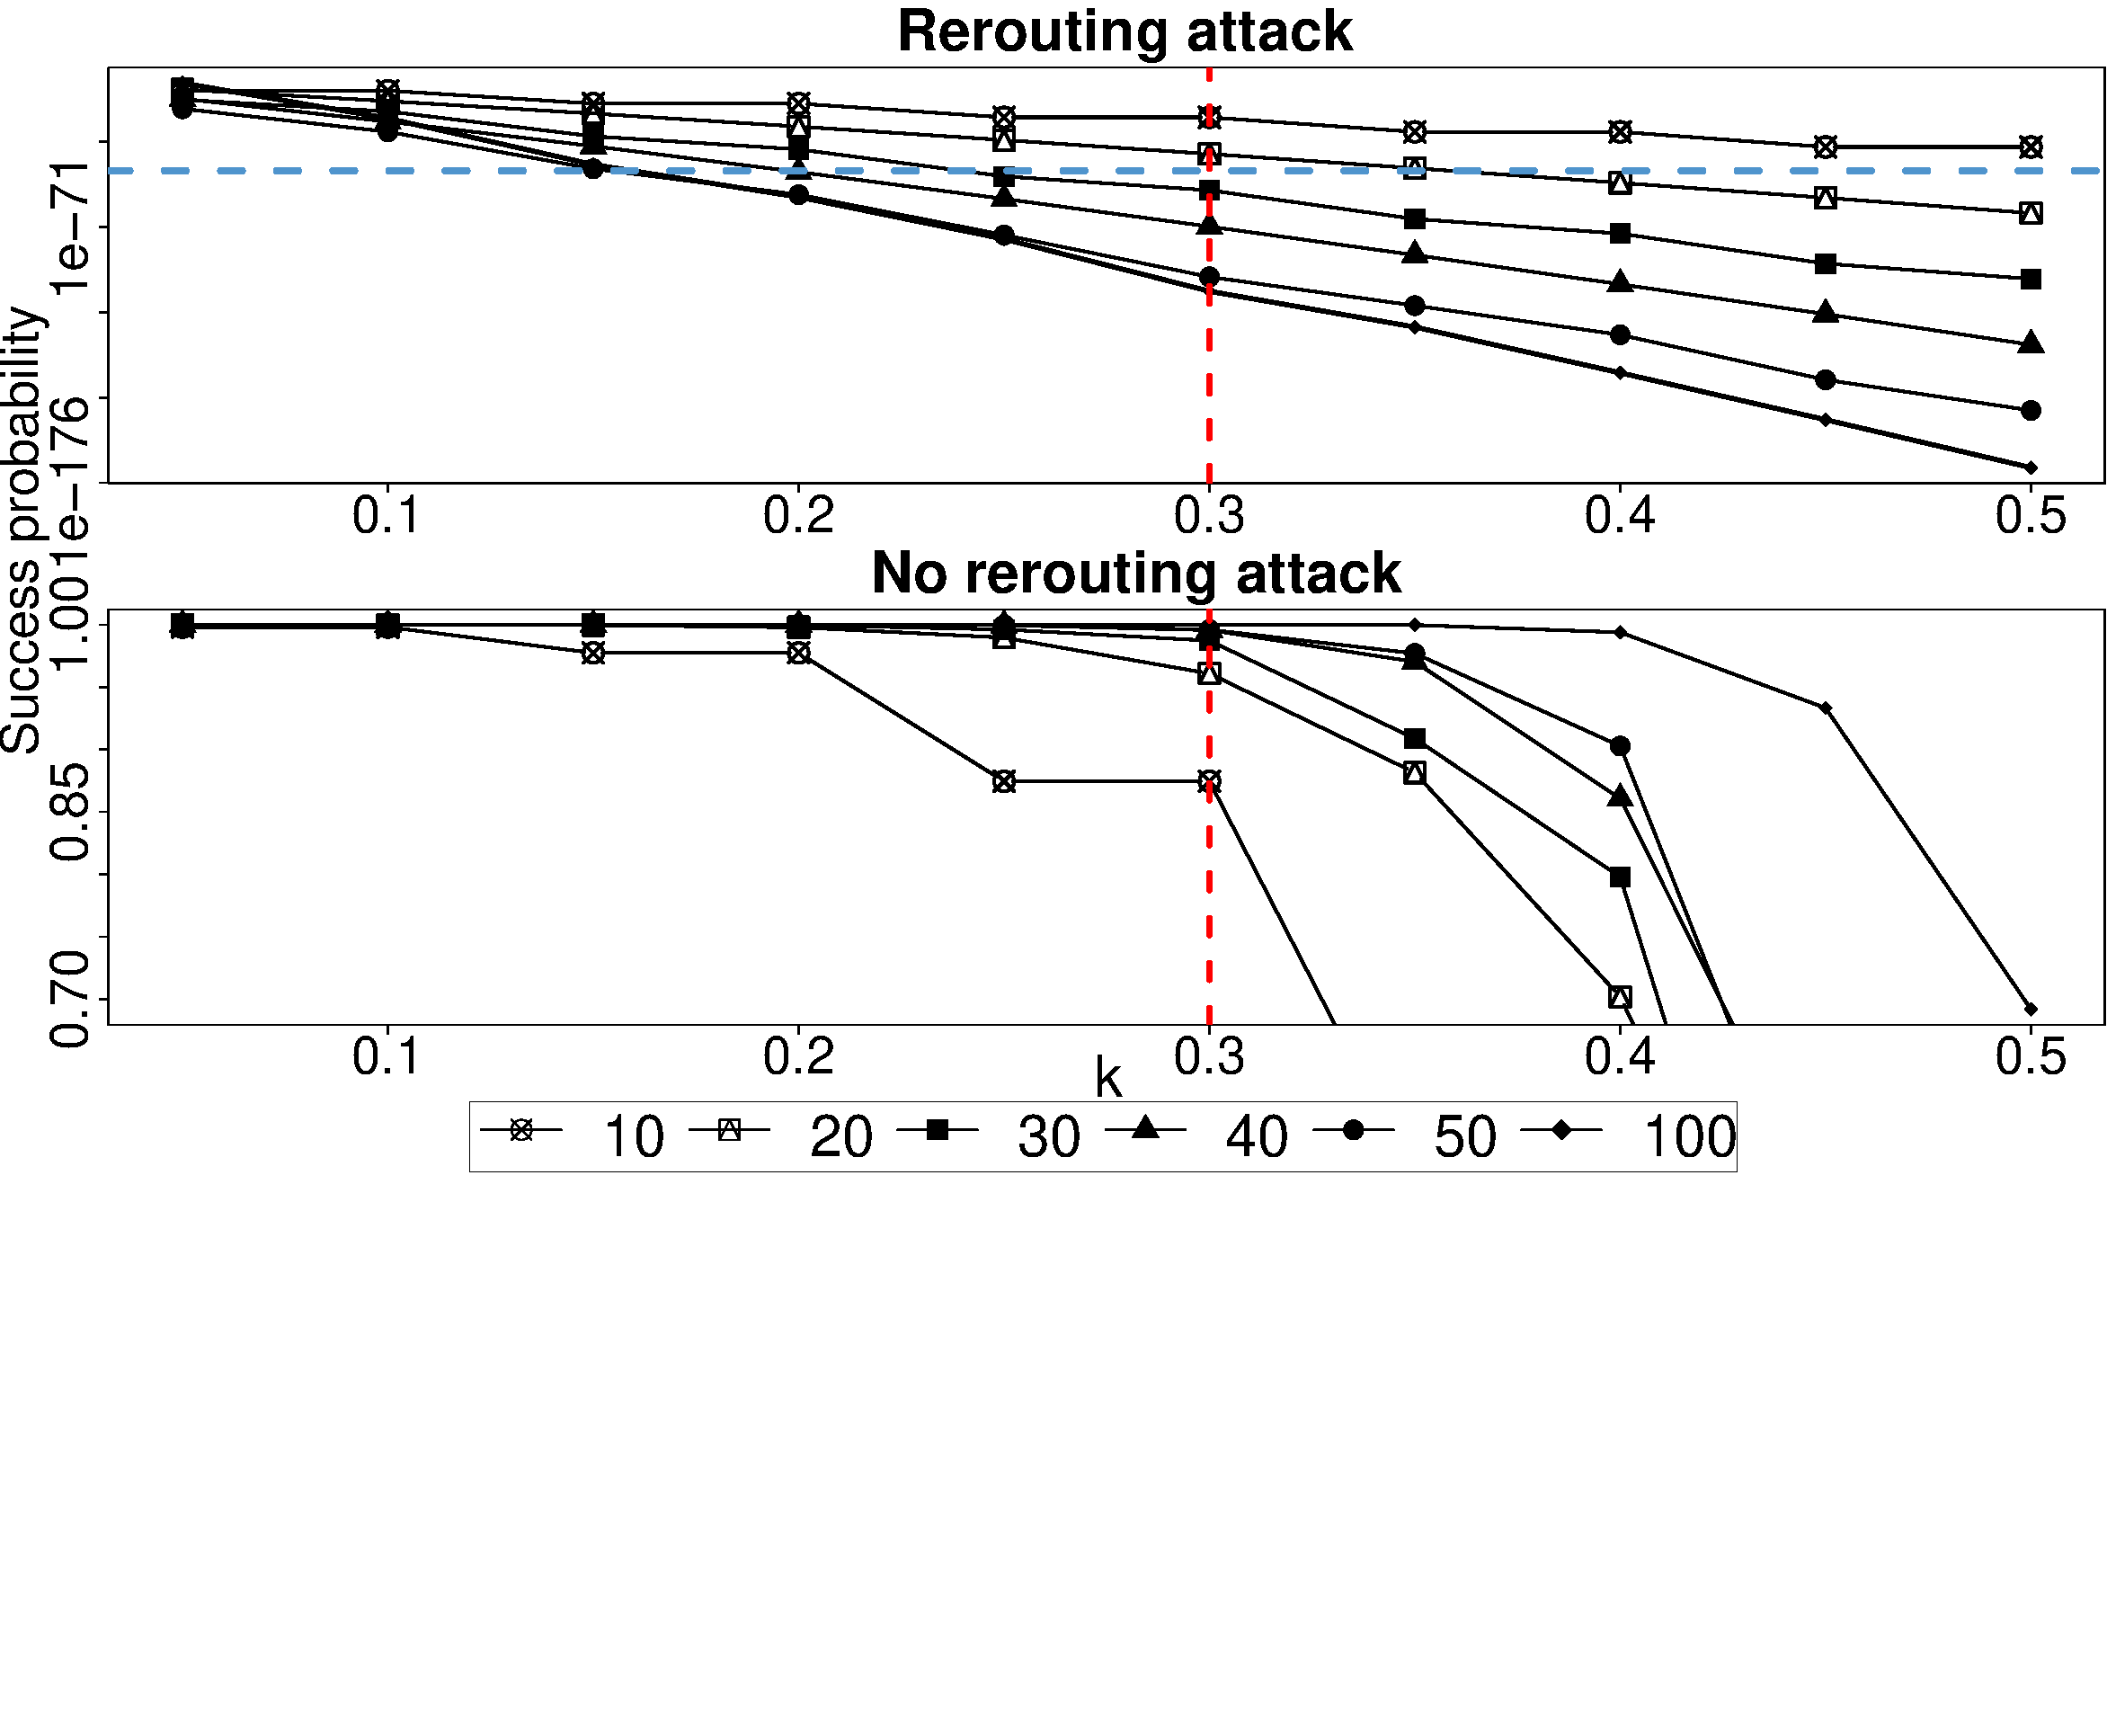
\includegraphics[trim={0 10.6cm 0 0}, clip, width=0.9\linewidth]{data/graph/round_comp_1.pdf}
    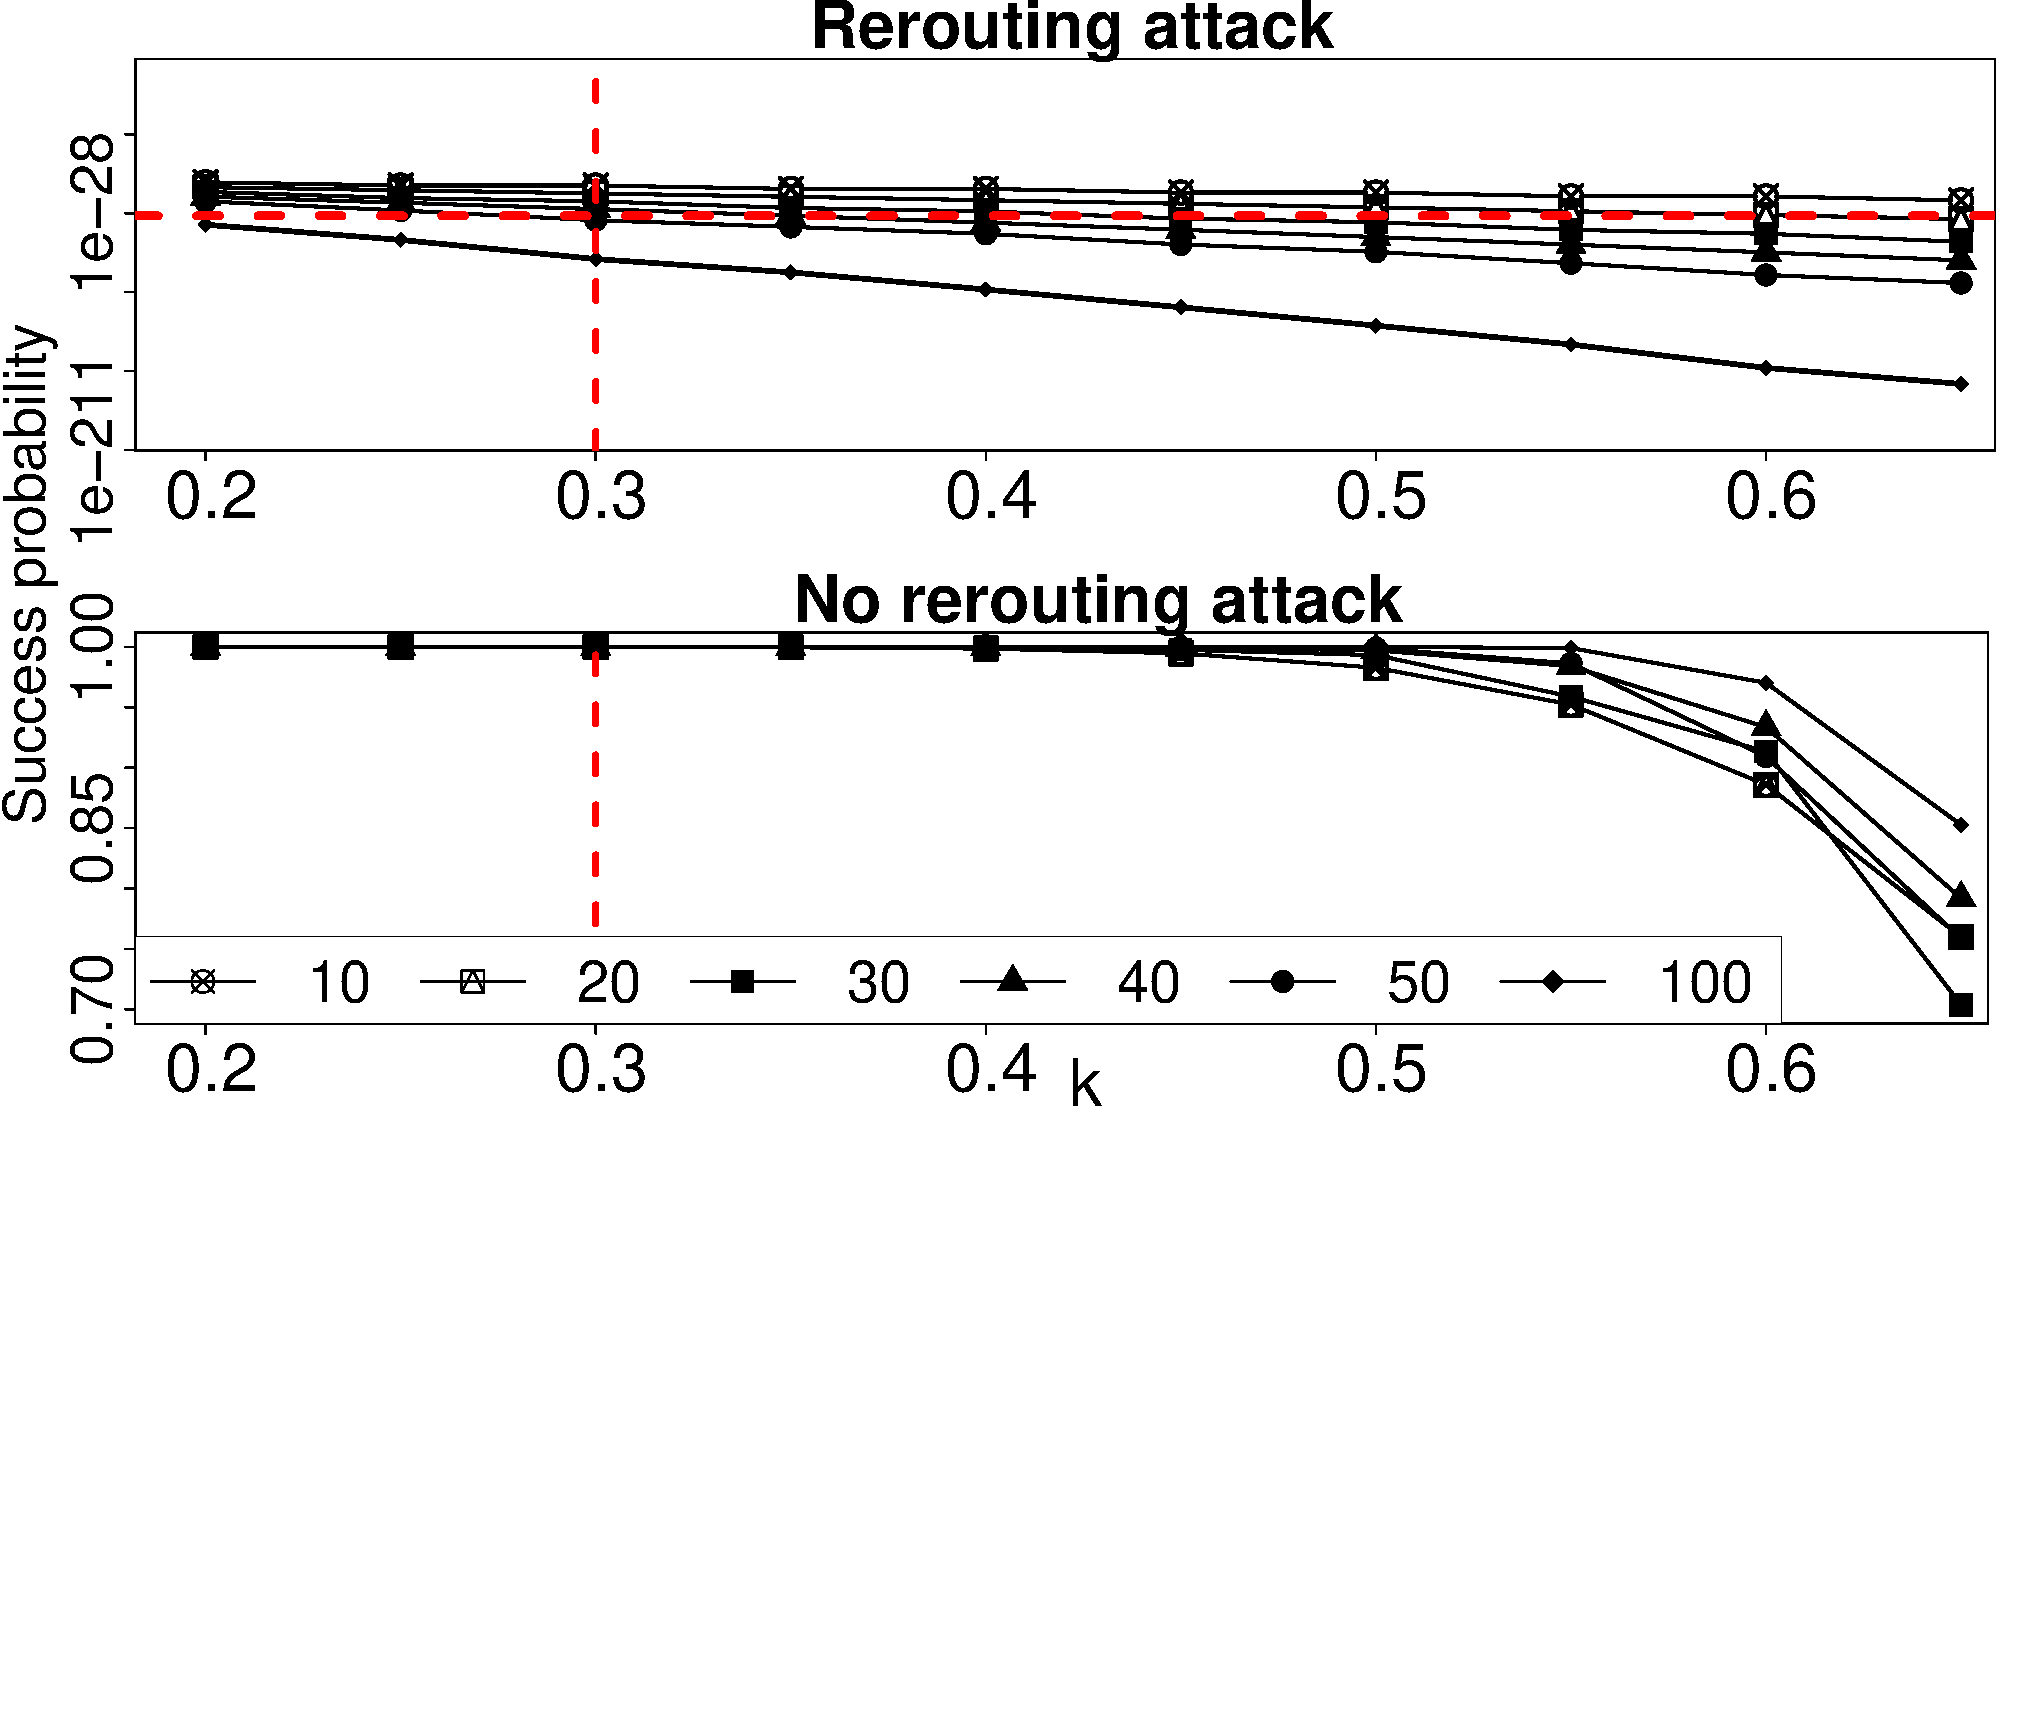
\includegraphics[trim={0 10cm 0 0}, clip, width=\linewidth]{data/fx3_data/round_comp_new.pdf}
    \caption{\roundCompCaption}
    %\vspace{-5px}
    \label{graph:roundSuccess}
\end{figure}


\myparagraph{2. Choosing a suitable fraction $k$.} The next step of the evaluation is to find a suitable fraction $k$ based on the threshold time \connect. Note that both the success probability of the attacker and the legitimate enclave is calculated as the cumulative probability from a binomial distribution (from $nk$ to $n$). Hence, we require to choose a suitable value of $k$ that maximizes $P_{legit}$ while minimizing $P_{adv}$.

We calculate two graphs that are depicted in Figure~\ref{graph:roundSuccess} where the x-axis denotes $k$, and the y-axis denotes attacker's success probability $P_{adv}$ and legitimate success probability $P_{legit}$, respectively, while using \connect$=186 \mu s$. We observe a sharp decrease in the legitimate success probability at $k=0.3$. Hence, fix $k=0.3$ to achieve the maximum $P_{legit}$. Additionally, in the graph of attacker's success probability, the red horizontal line is placed at $10^{-30} \approx 2^{-100}$. Hence we propose to choose any round configuration bellow this horizontal line, where $n \geq 40$. With number of rounds set to $n=50$ and $k=0.3$, we have $P_{legit}=0.99999997$ and $P_{adv}=3.55\times 10^{-34}$. Similar result could be also observed in Figure~\ref{graph:roundSuccess} where the success probability of the legitimate enclave decreases significantly after $k=0.55$ for \connect$=186\mu s$.



\myparagraph{3. Generalizing the number of rounds $n$.} Figure~\ref{graph:instatAttackerHisto} extends this analysis to the general number of challenge-response rounds spanning from $n=2$ to $100$. Here we compute the probability of attacker returning the reply within $186 \mu s$ for at least $k=0.3$ fraction of challenges. The y-axis denotes the attacker's success probability which diminishes overwhelmingly with the increasing number of challenges (keeping the fraction constant at $k=0.3$). 




\newcommand{\timeRoundCaption}{\textbf{Effect of different threshold latencies (\connect).} The figure shows the success probability when no relay attack takes place. The threshold latency \connect $=470\ \mu s$ reaches to $0.999999965$ success probability for number of trials at least 20 ($k.n,\ k=0.4$) out of $n=50$ challenge-response protocol.}

\newcommand{\cumulativeCaption}{\textbf{Cumulative distribution function for latencies.} We set the threshold \connect at 470 $\mu s$ which has a cumulative probability of $0.75$ in the experiment where no rerouting attack takes place with an extremely low probability ($9.73\times10^{-5}$).}

\ifusenix
\begin{figure}[t]
  \centering
   % 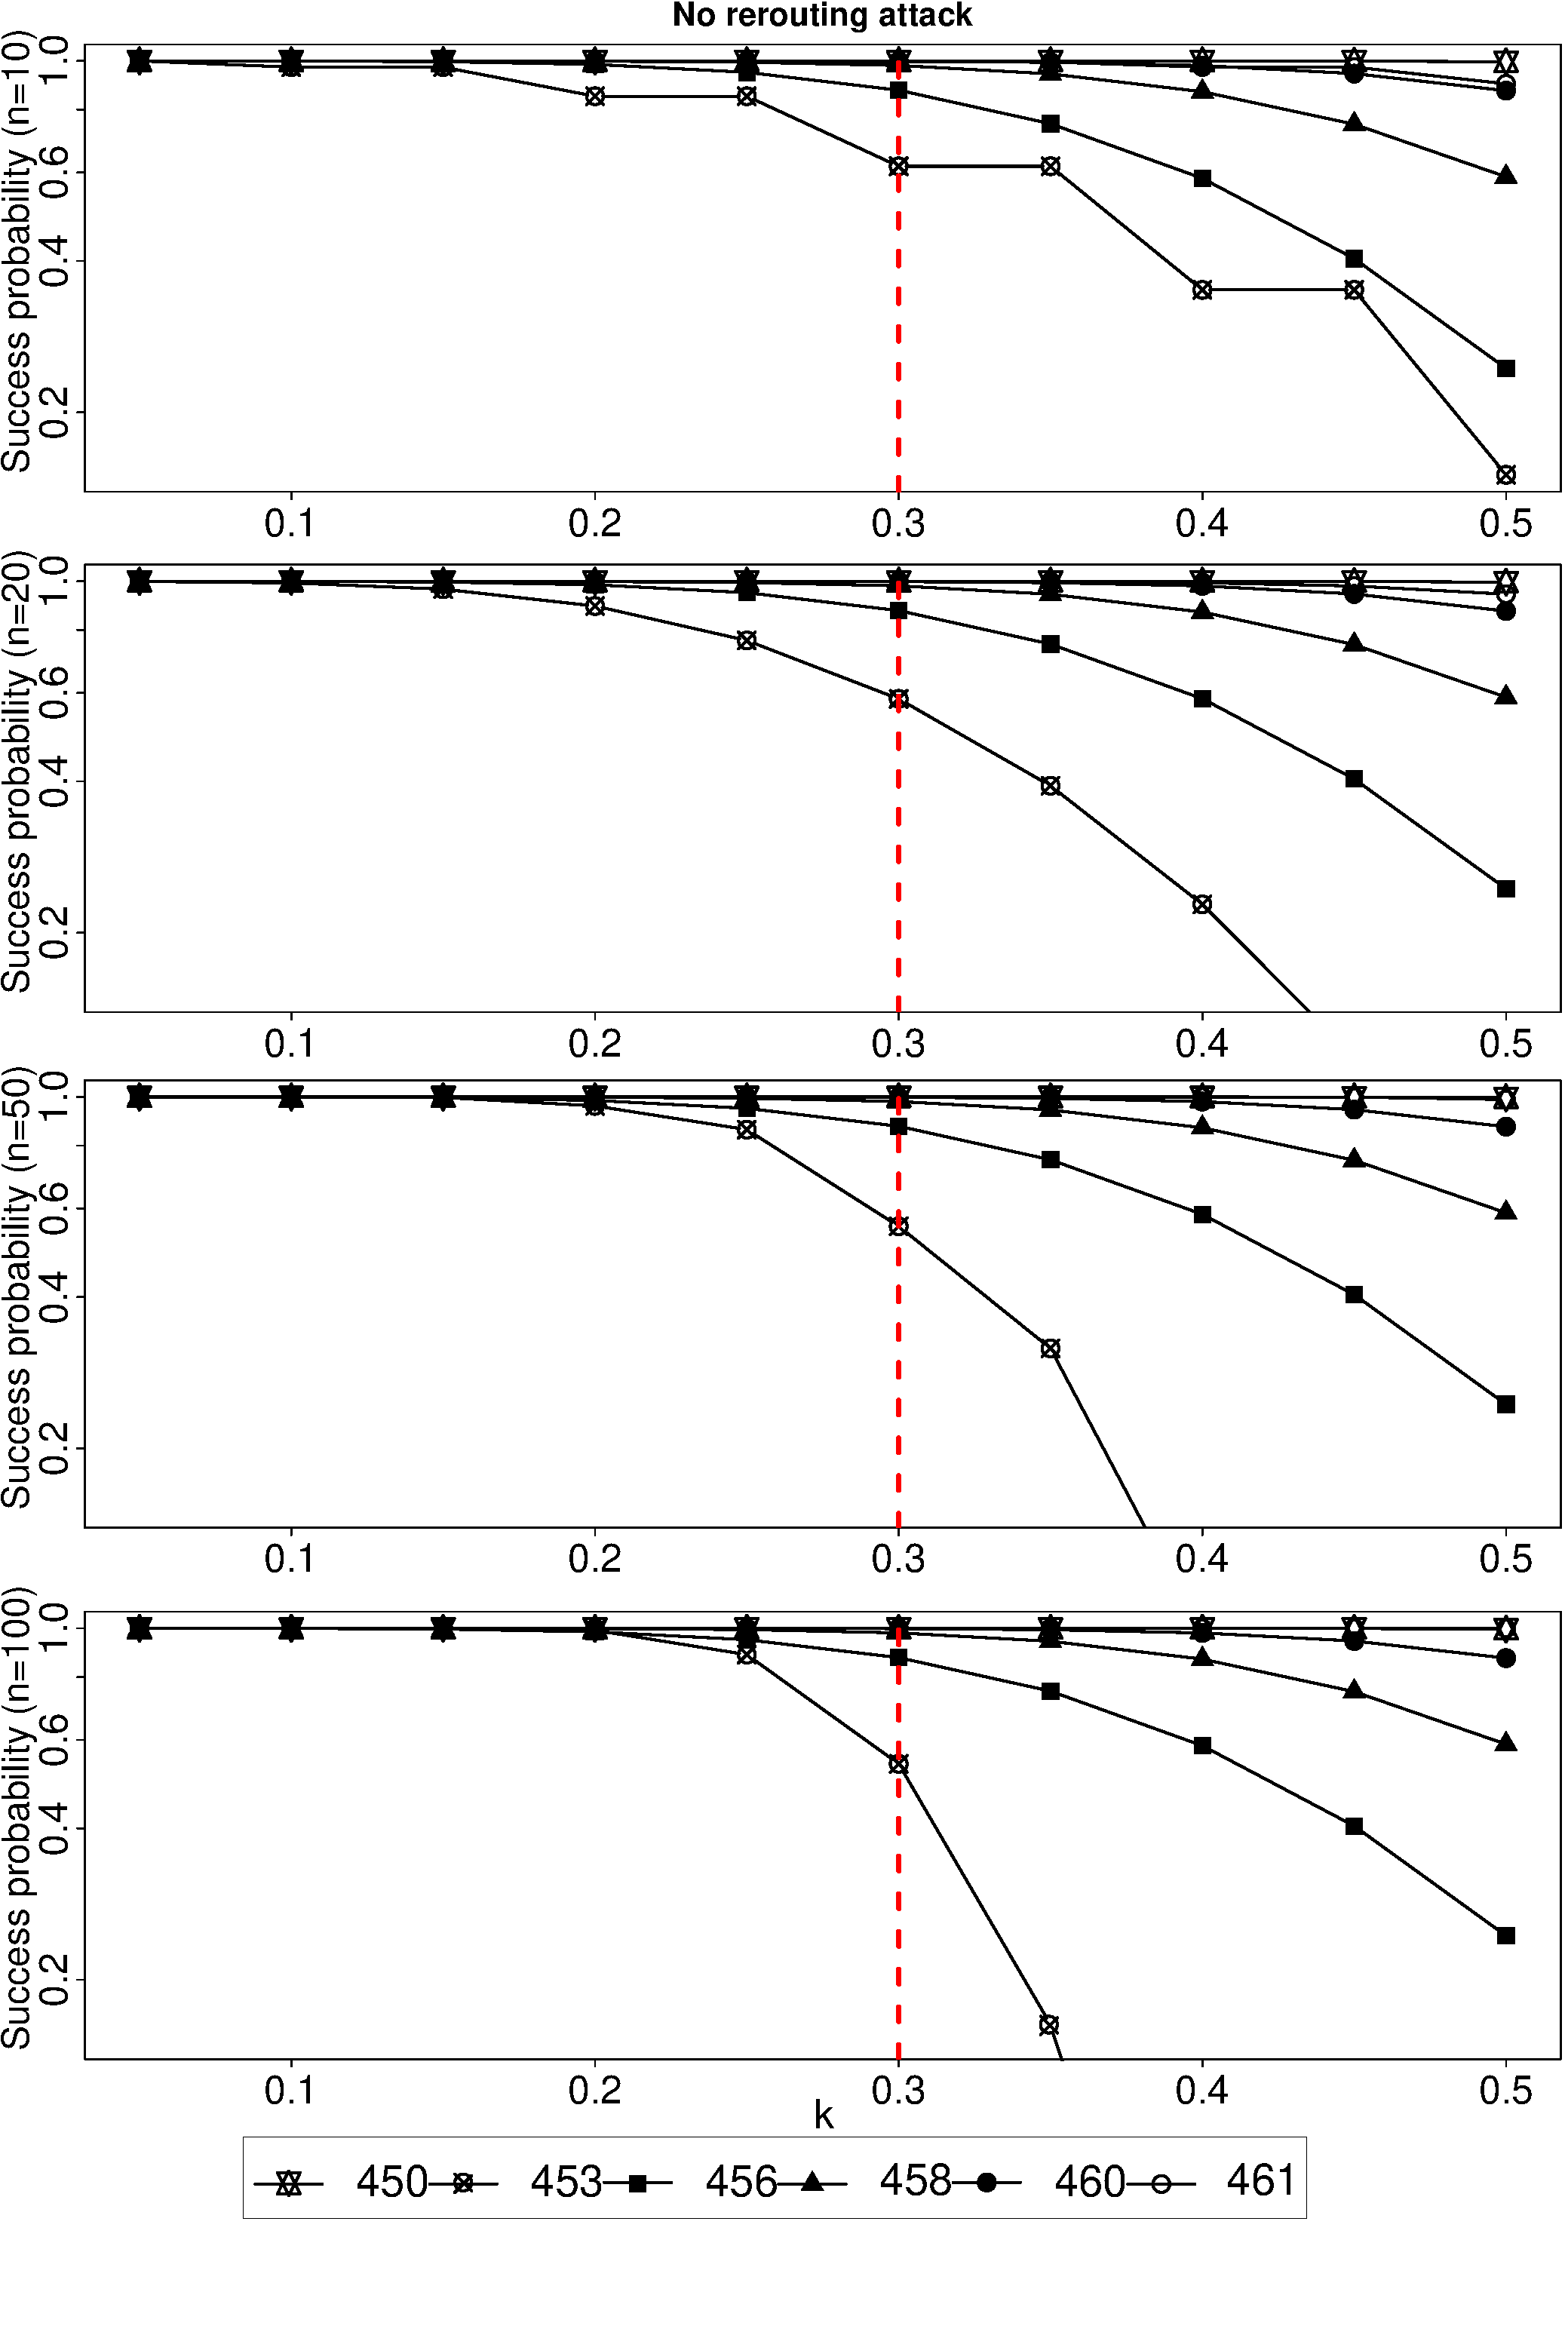
\includegraphics[trim={0 2cm 0 0}, clip, width=0.95\linewidth]{data/graph/timeRound.pdf}
    %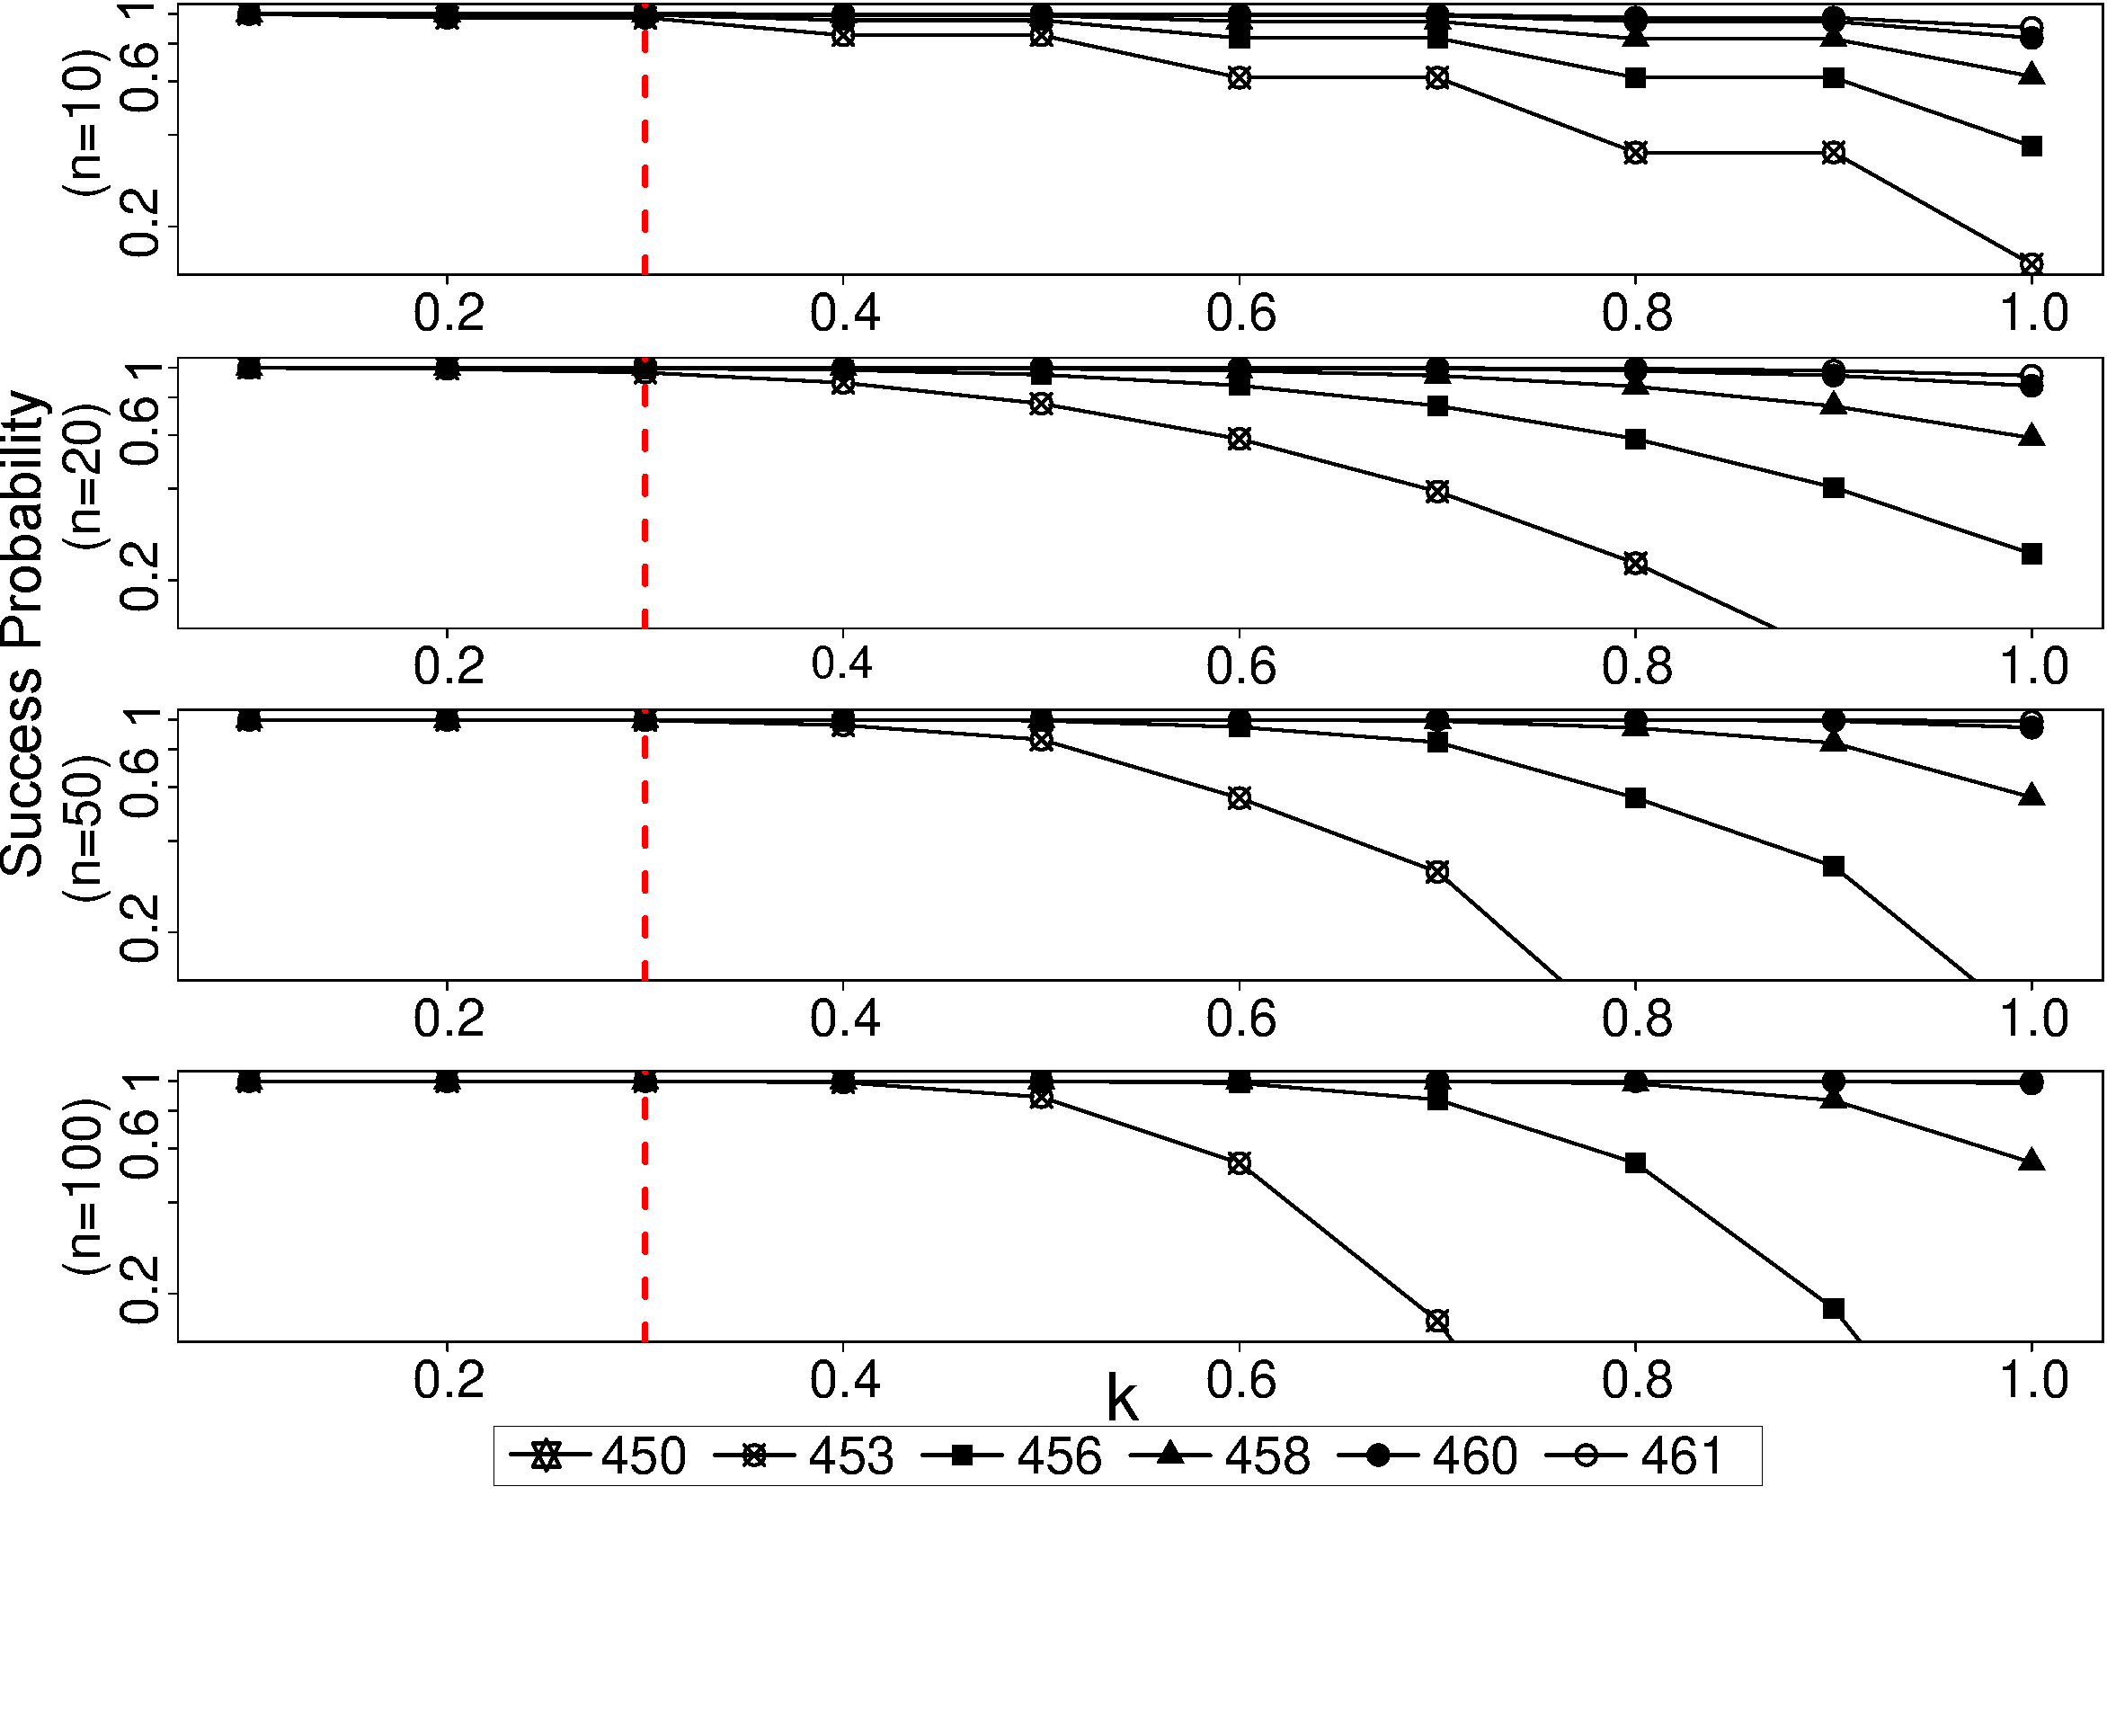
\includegraphics[trim={0 4.7cm 0 0}, clip, width=\linewidth]{data/graph/timeRound_1.pdf}
    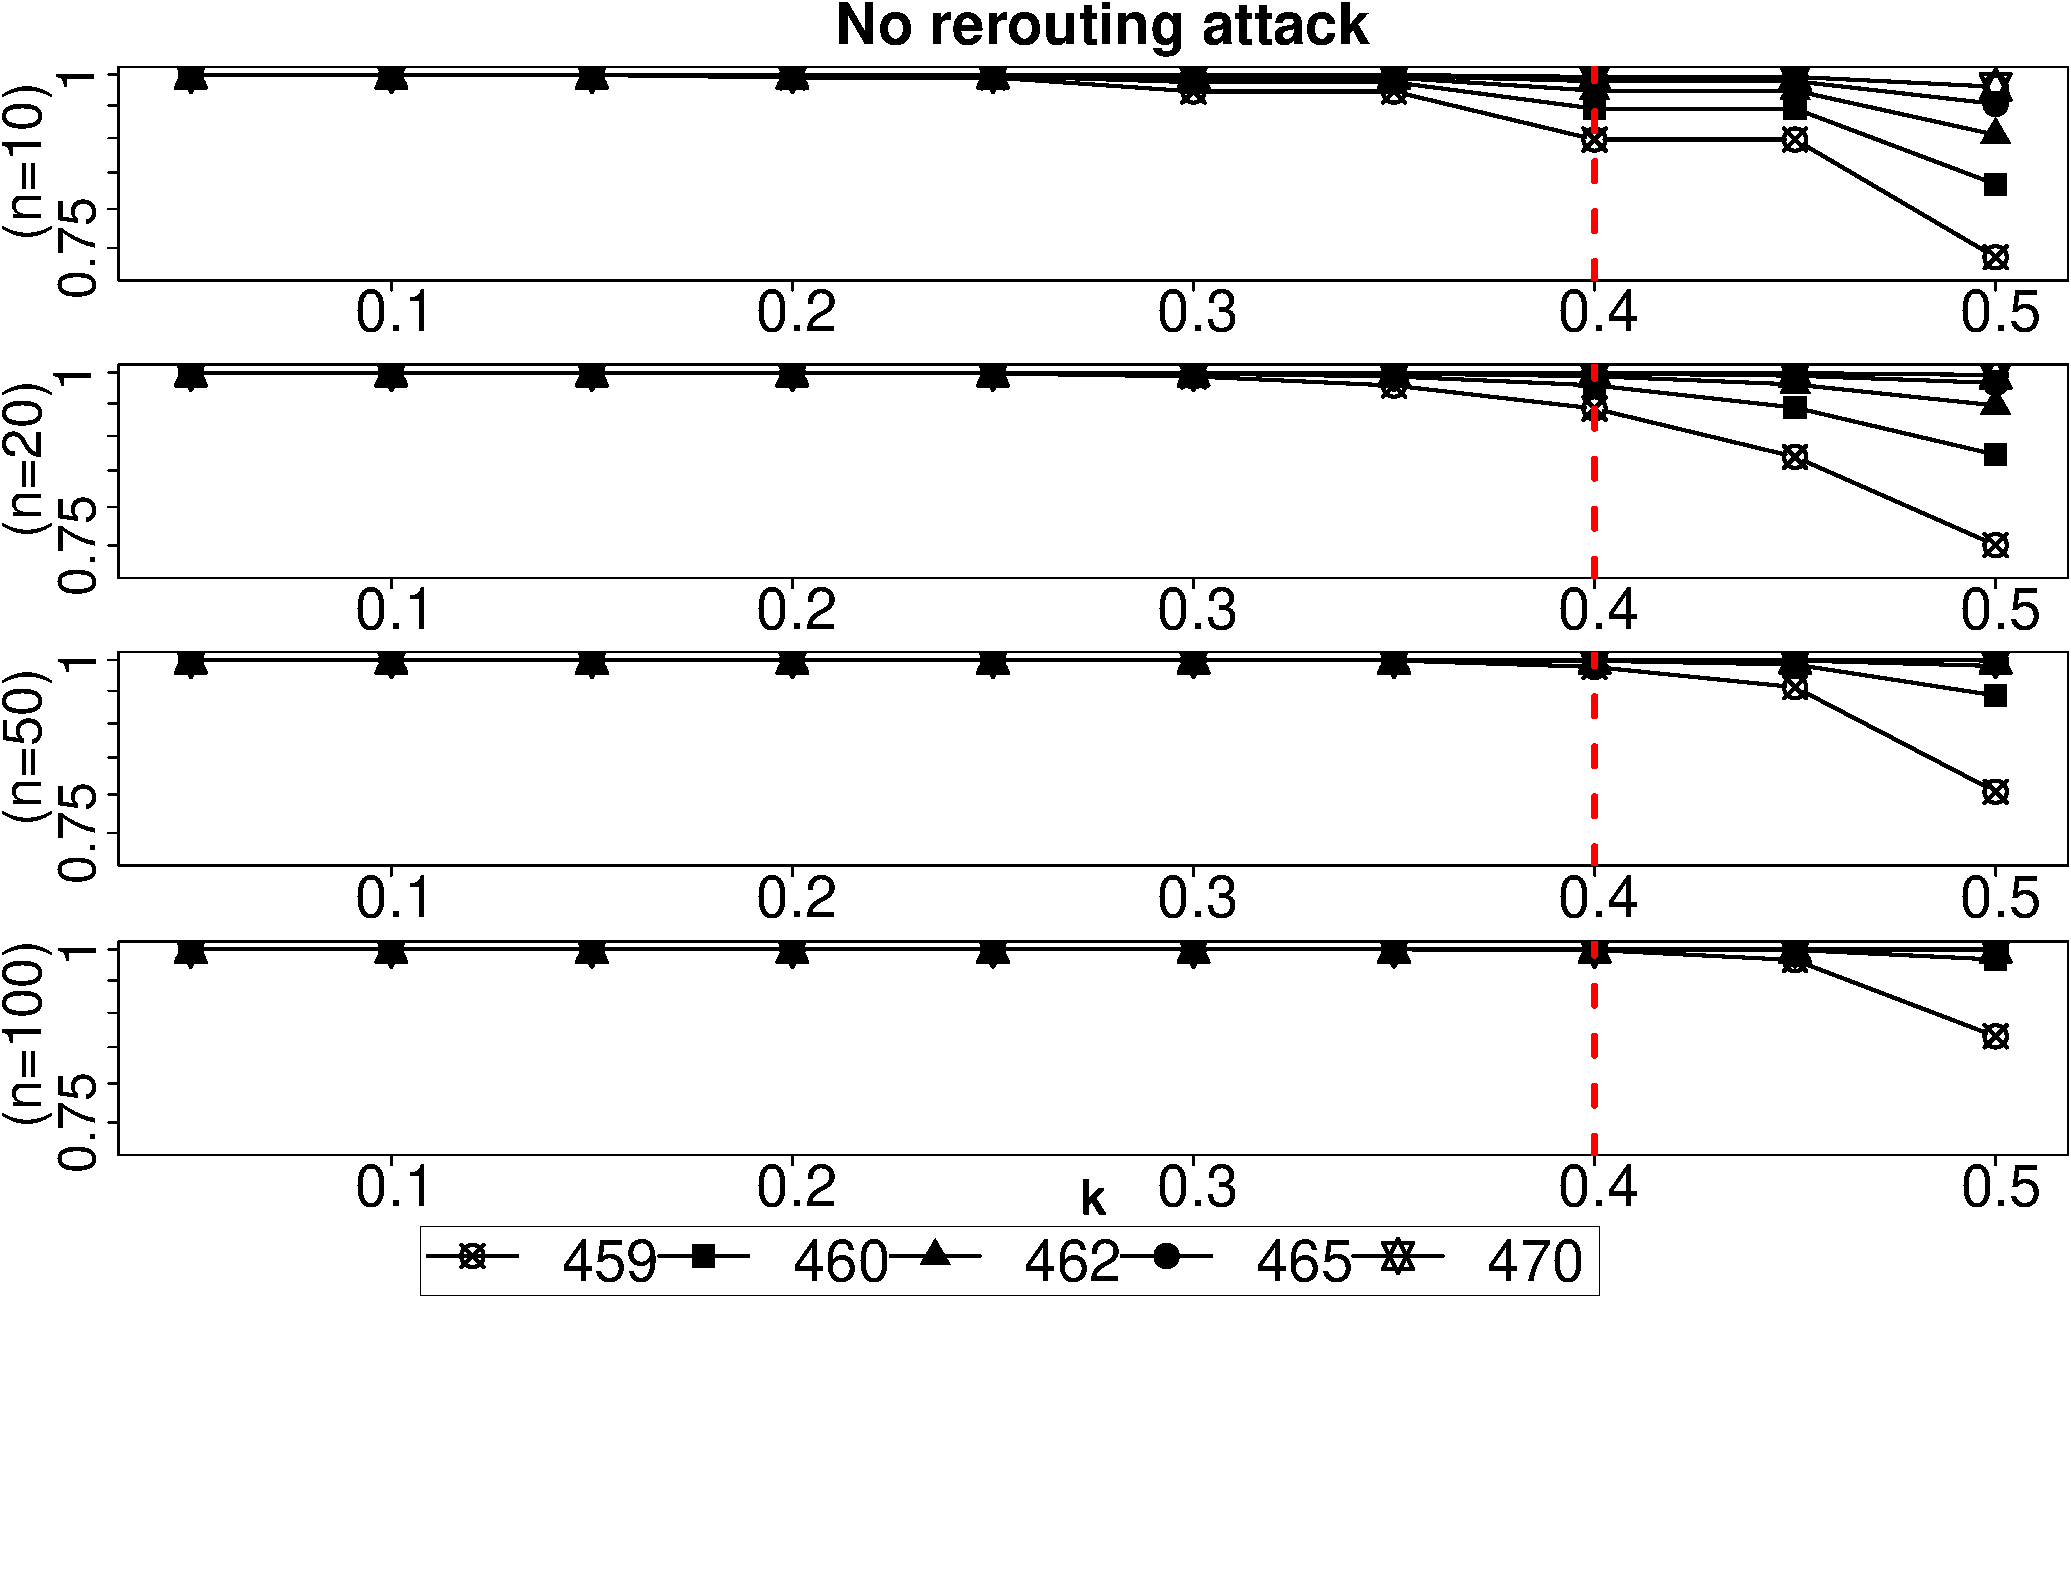
\includegraphics[trim={0 5cm 0 0}, clip, width=\linewidth]{data/graph/timeRound_new.pdf}
    \caption{\timeRoundCaption}
   %\vspace{-5px}
    \label{graph:diffTh}
\end{figure}

\begin{figure}[t]
  \centering
    %\includegraphics[trim={0 0 0 0}, clip, width=0.4\linewidth]{data/graph/CDF_Latency.pdf}
    %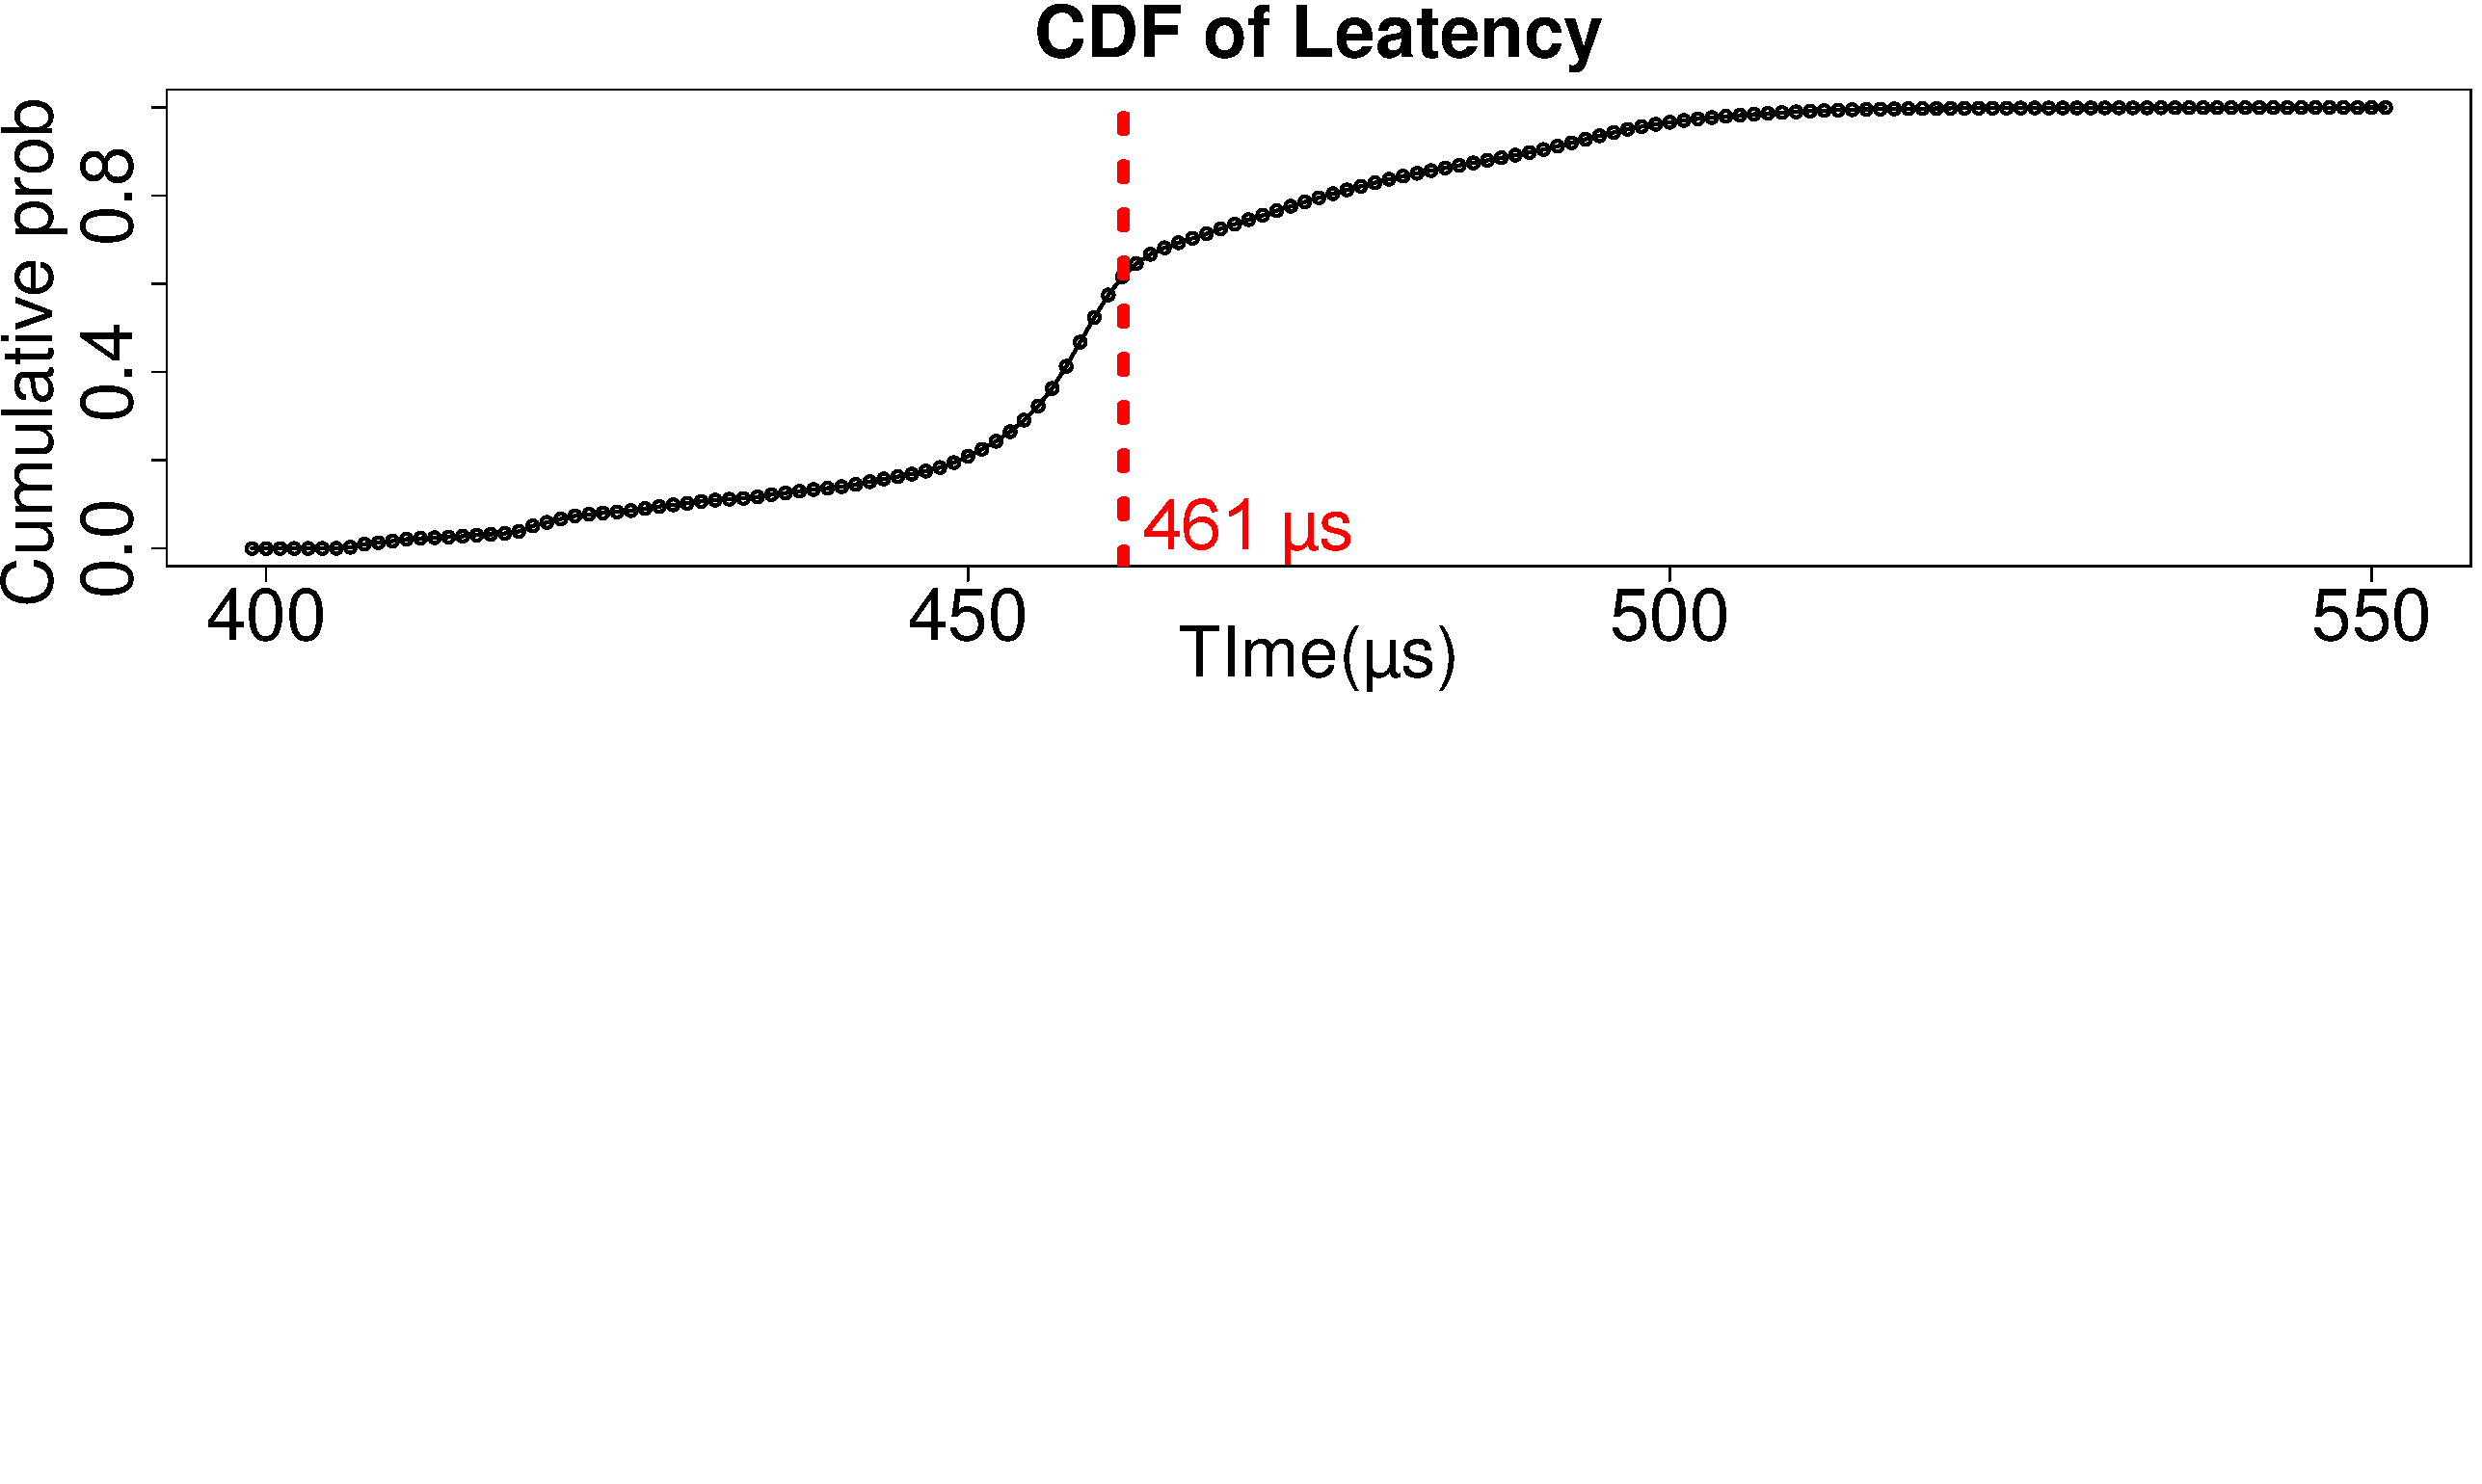
\includegraphics[trim={0 14cm 0 0}, clip, width=\linewidth]{data/graph/CDF_Latency1.pdf}
    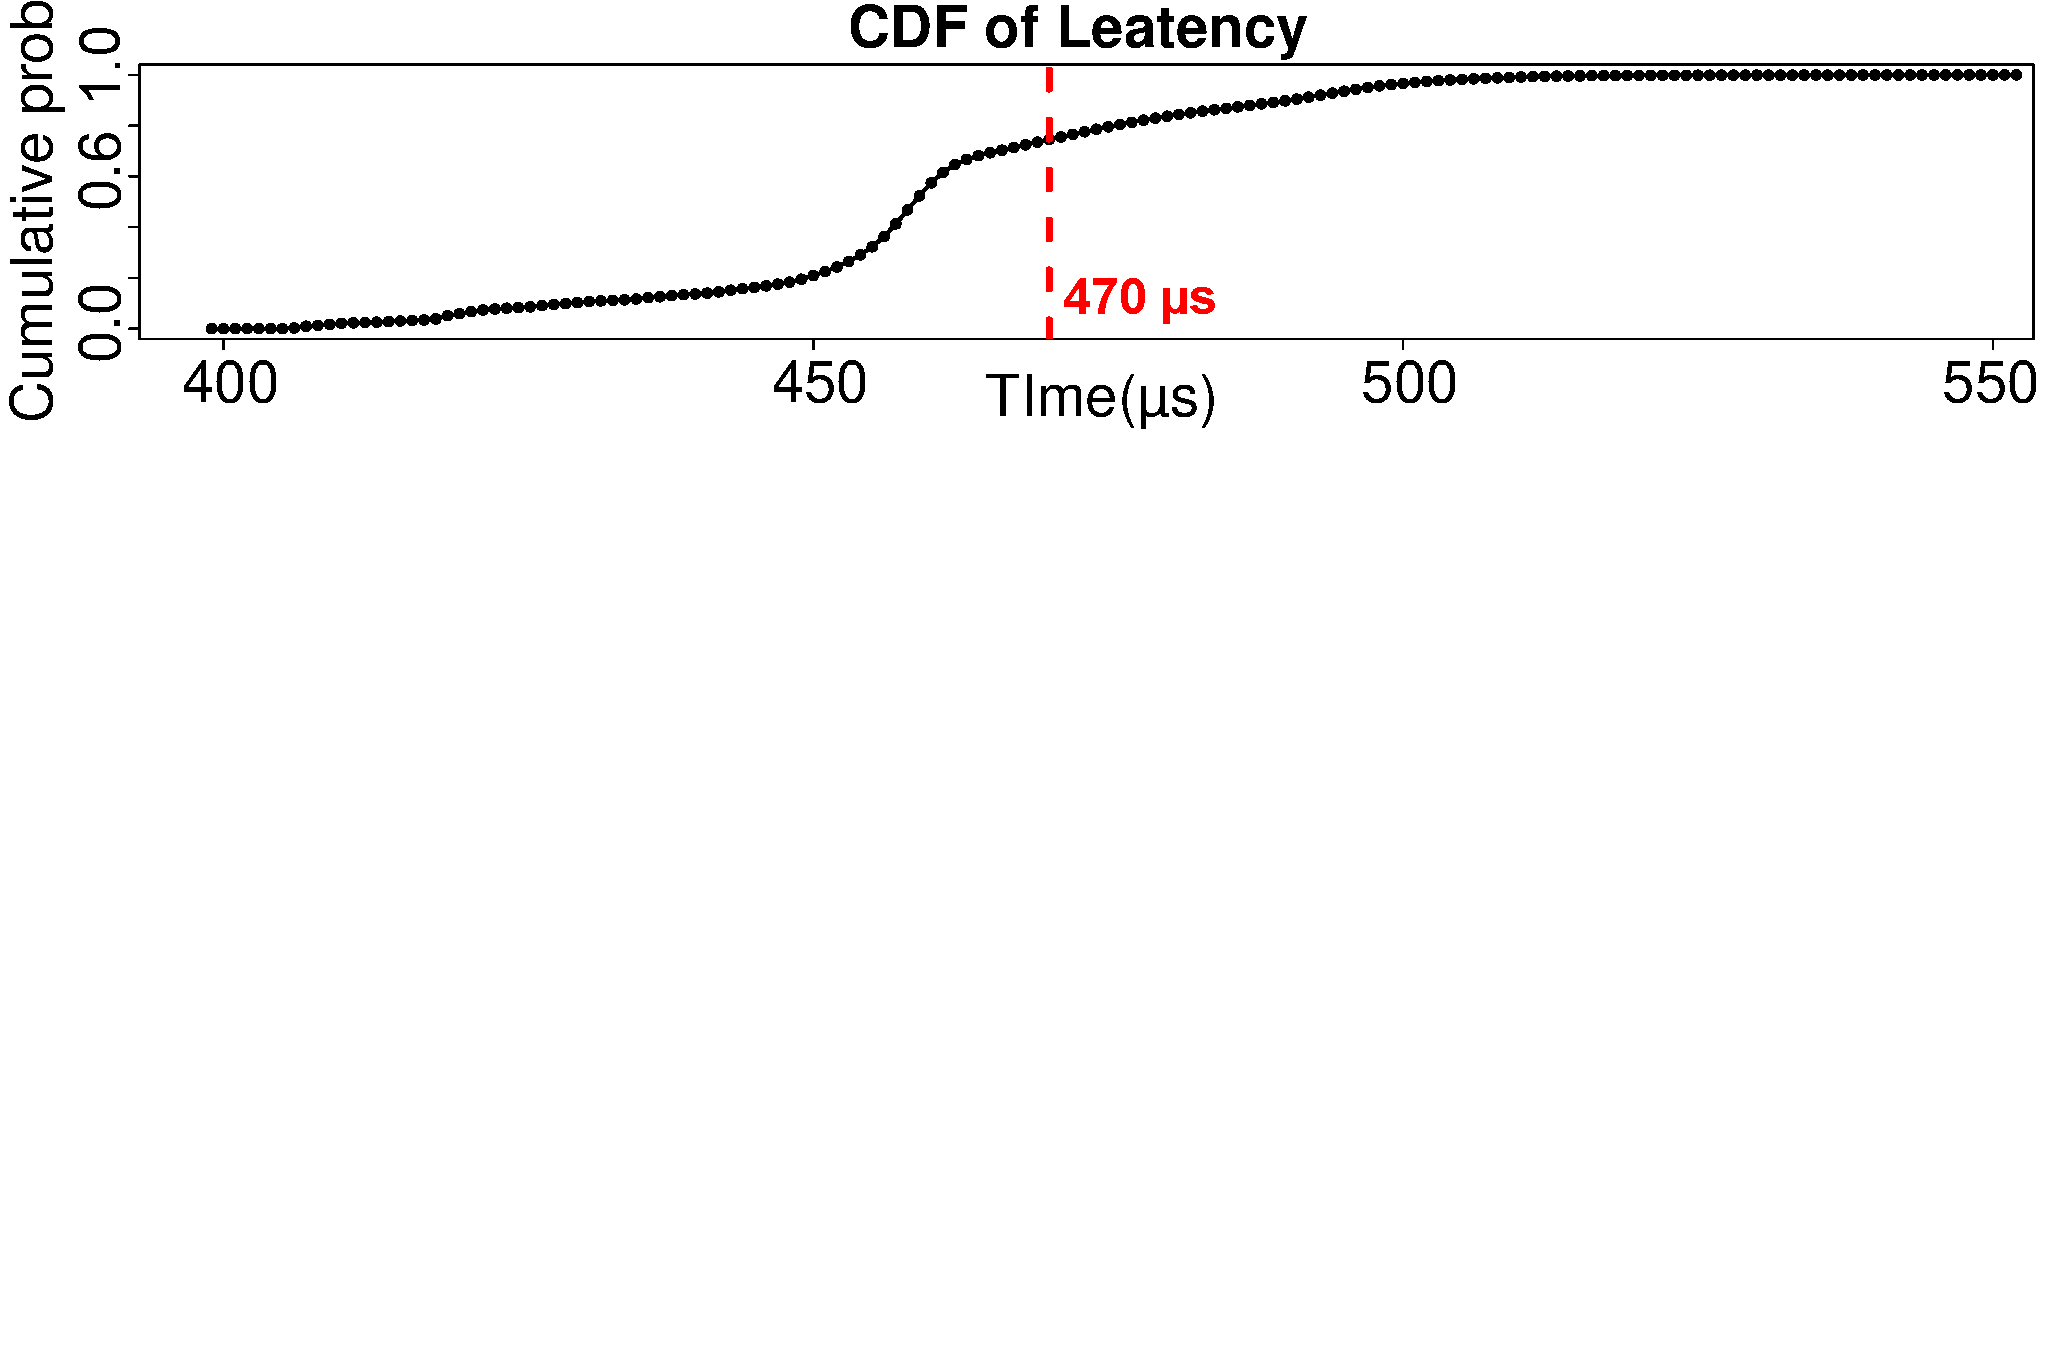
\includegraphics[trim={0 16cm 0 0}, clip, width=\linewidth]{data/graph/CDF_Latency_new.pdf}
    \caption{\cumulativeCaption}
    \vspace{-10px}
    \label{fig:cdf}
\end{figure}

\else

\begin{figure*}[t!]
    \centering
    \begin{subfigure}[t]{0.66\textwidth}
        \centering
        %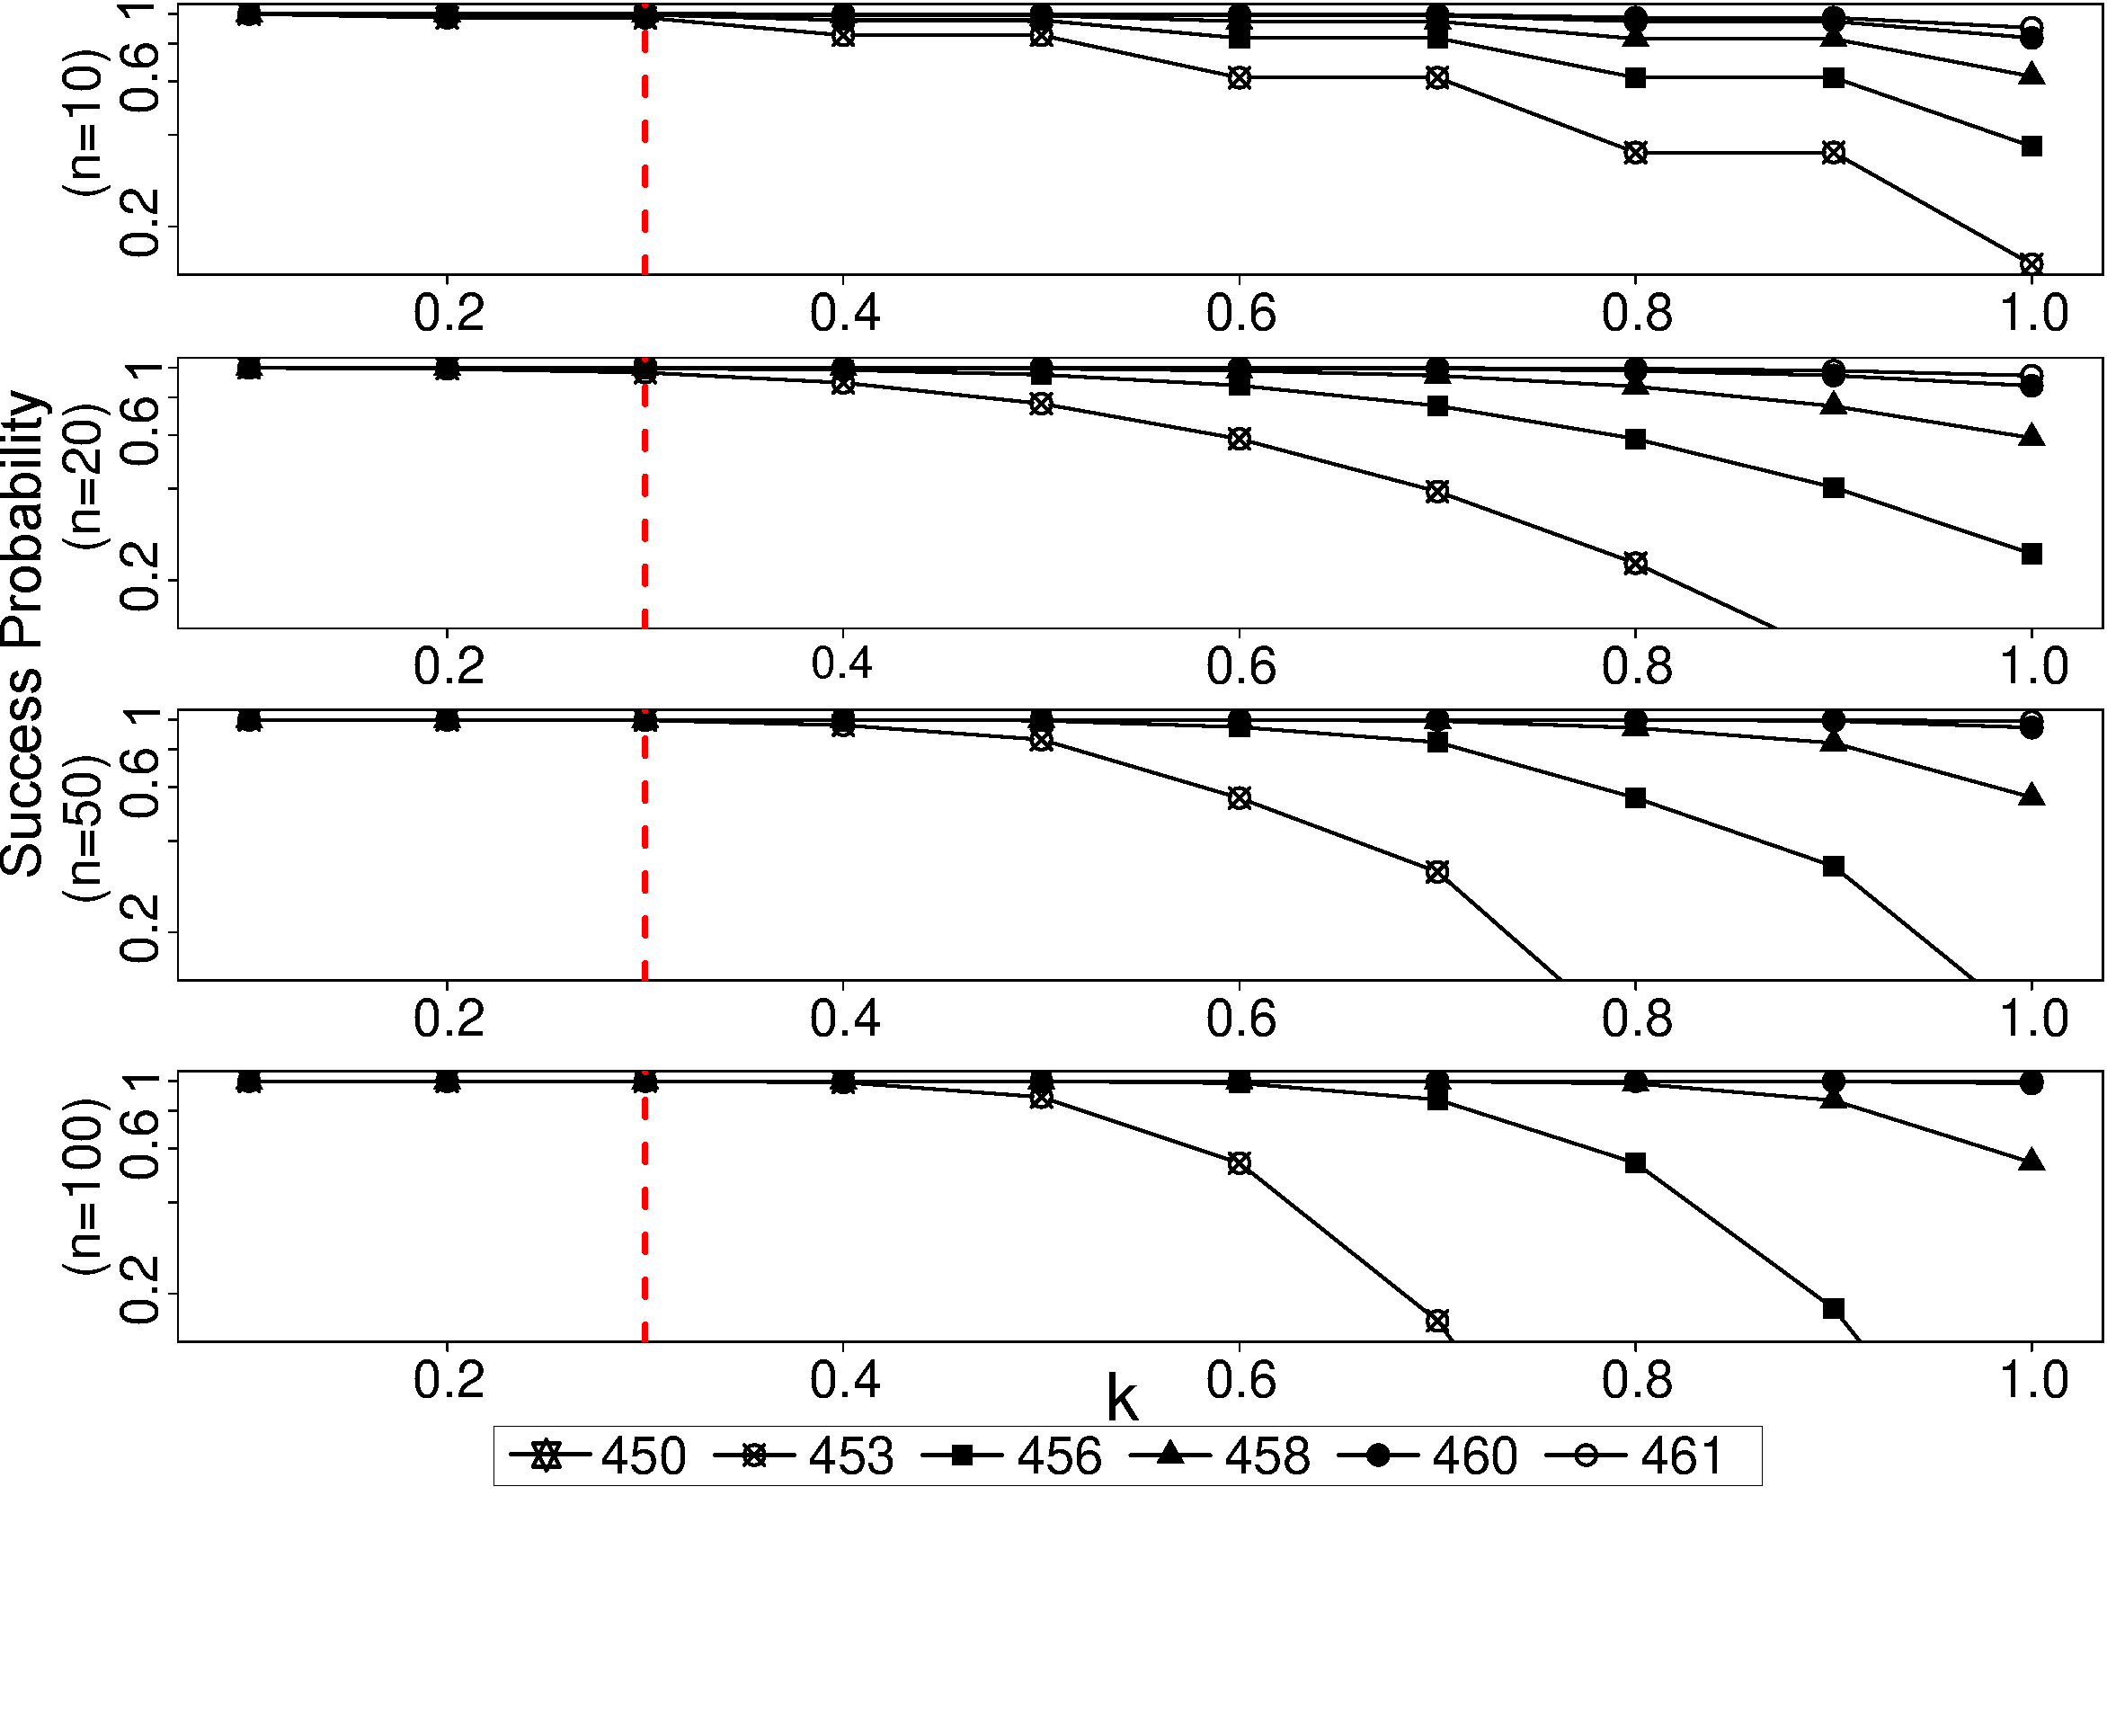
\includegraphics[trim={0 4.7cm 0 0}, clip,  height=2.6in]{data/graph/timeRound_1.pdf}
        %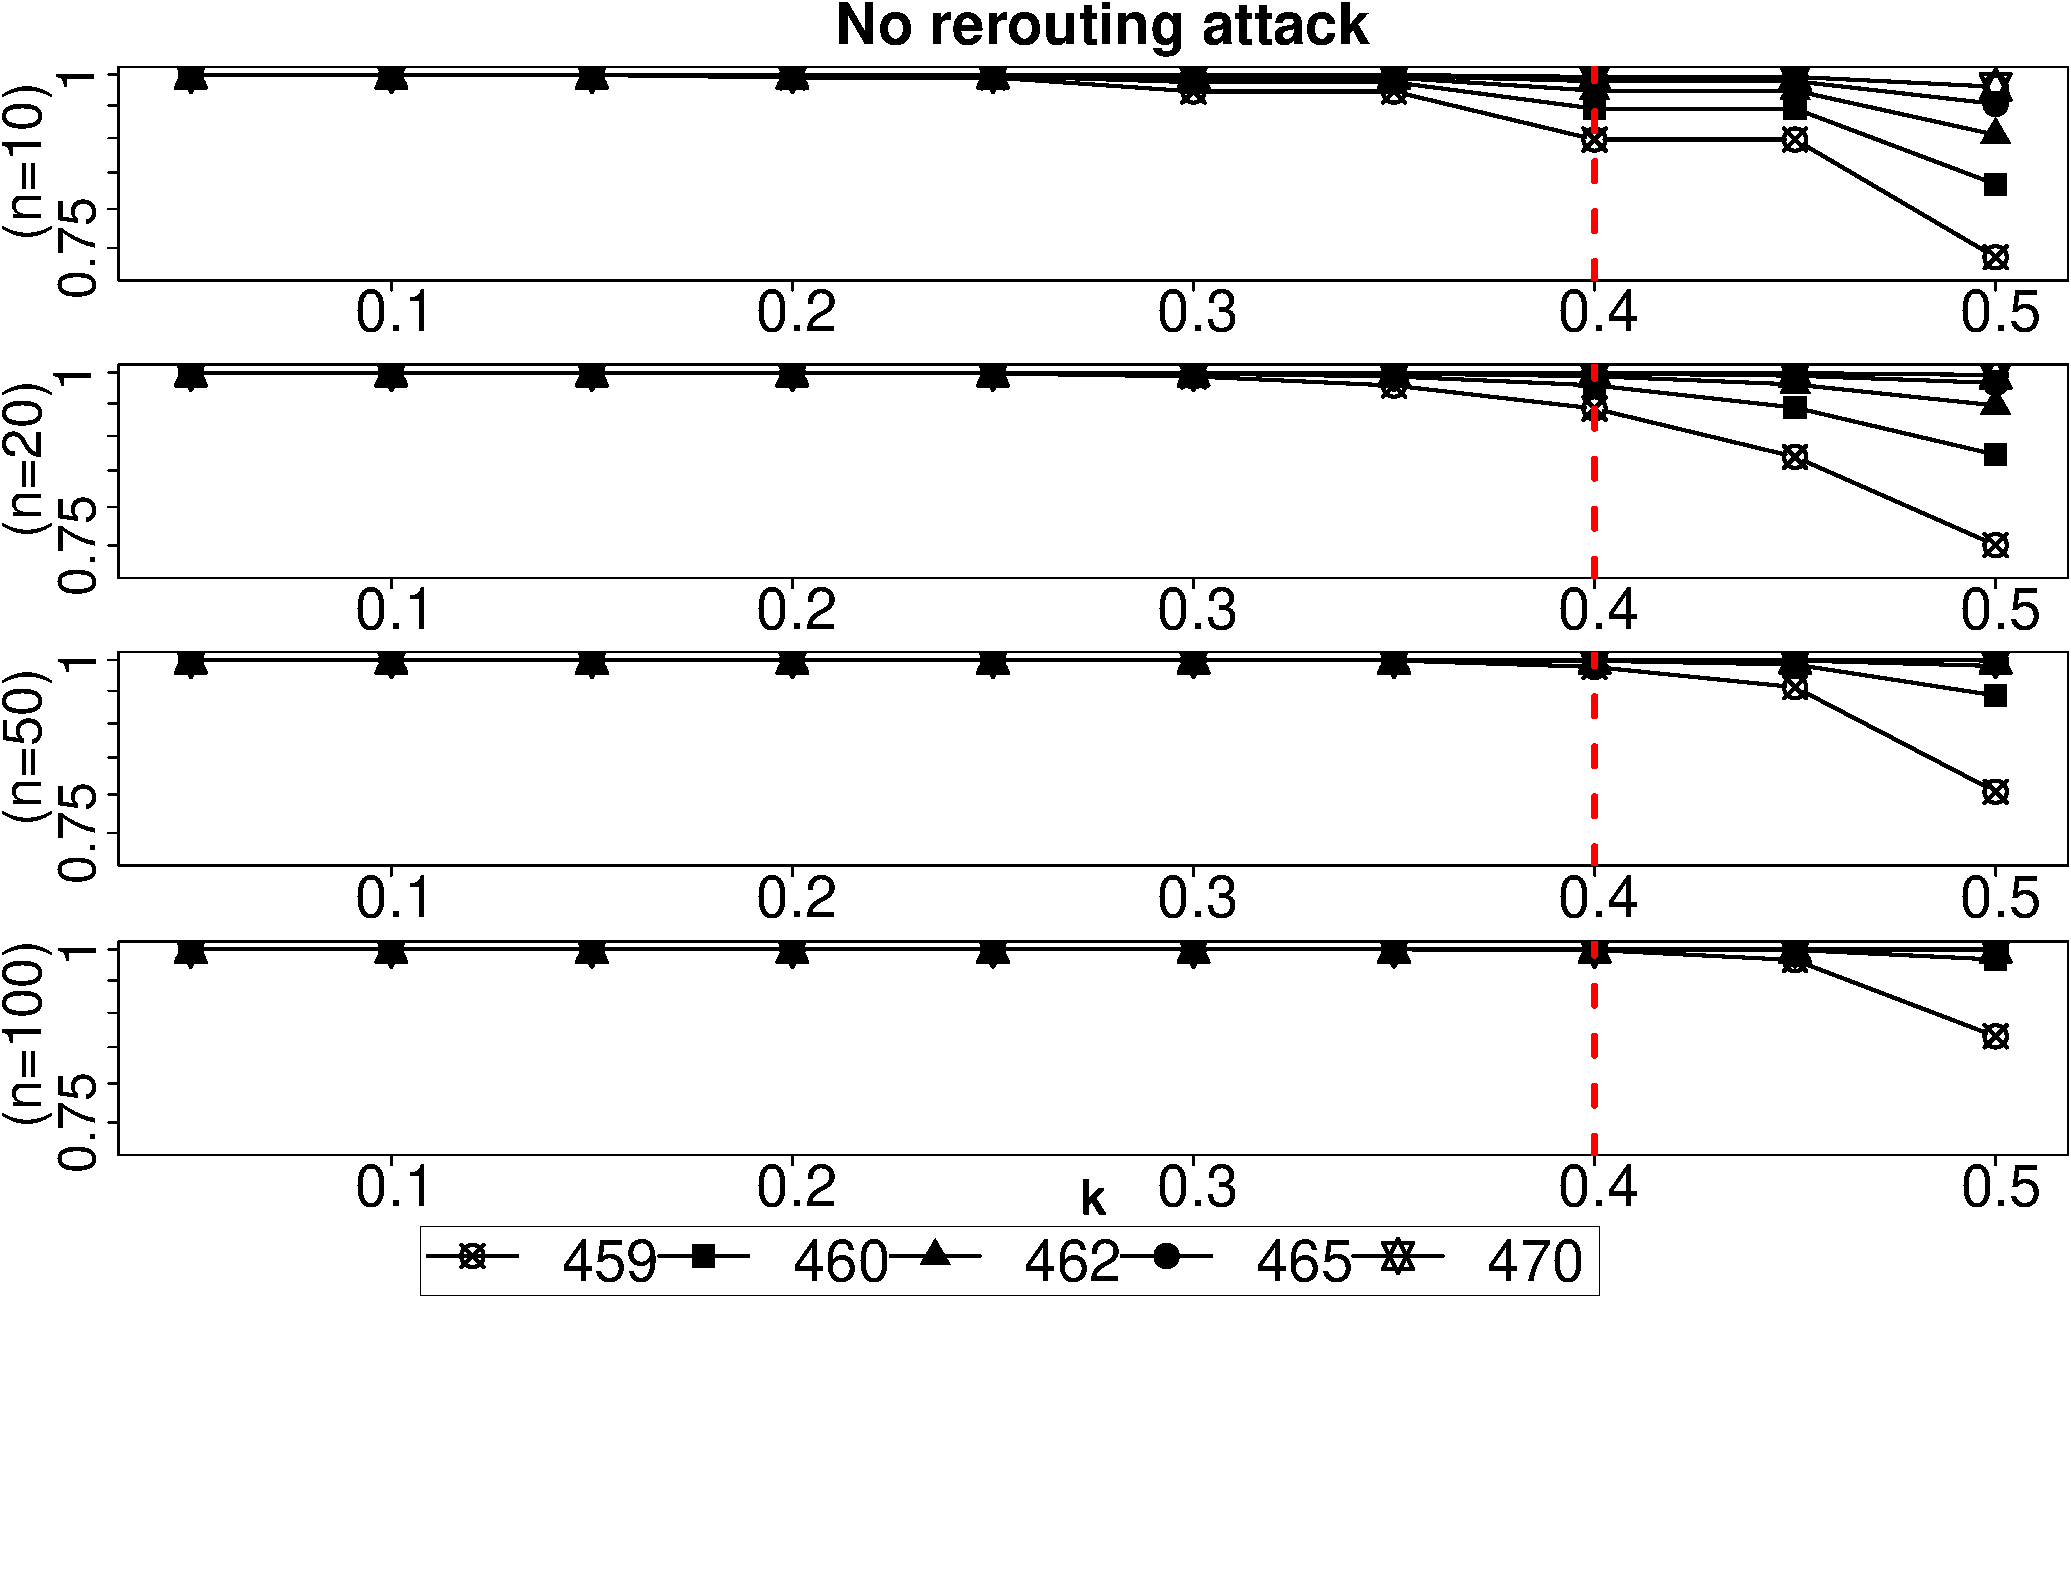
\includegraphics[trim={0 4.7cm 0 0}, clip,  height=2.6in]{data/graph/timeRound_new.pdf}
         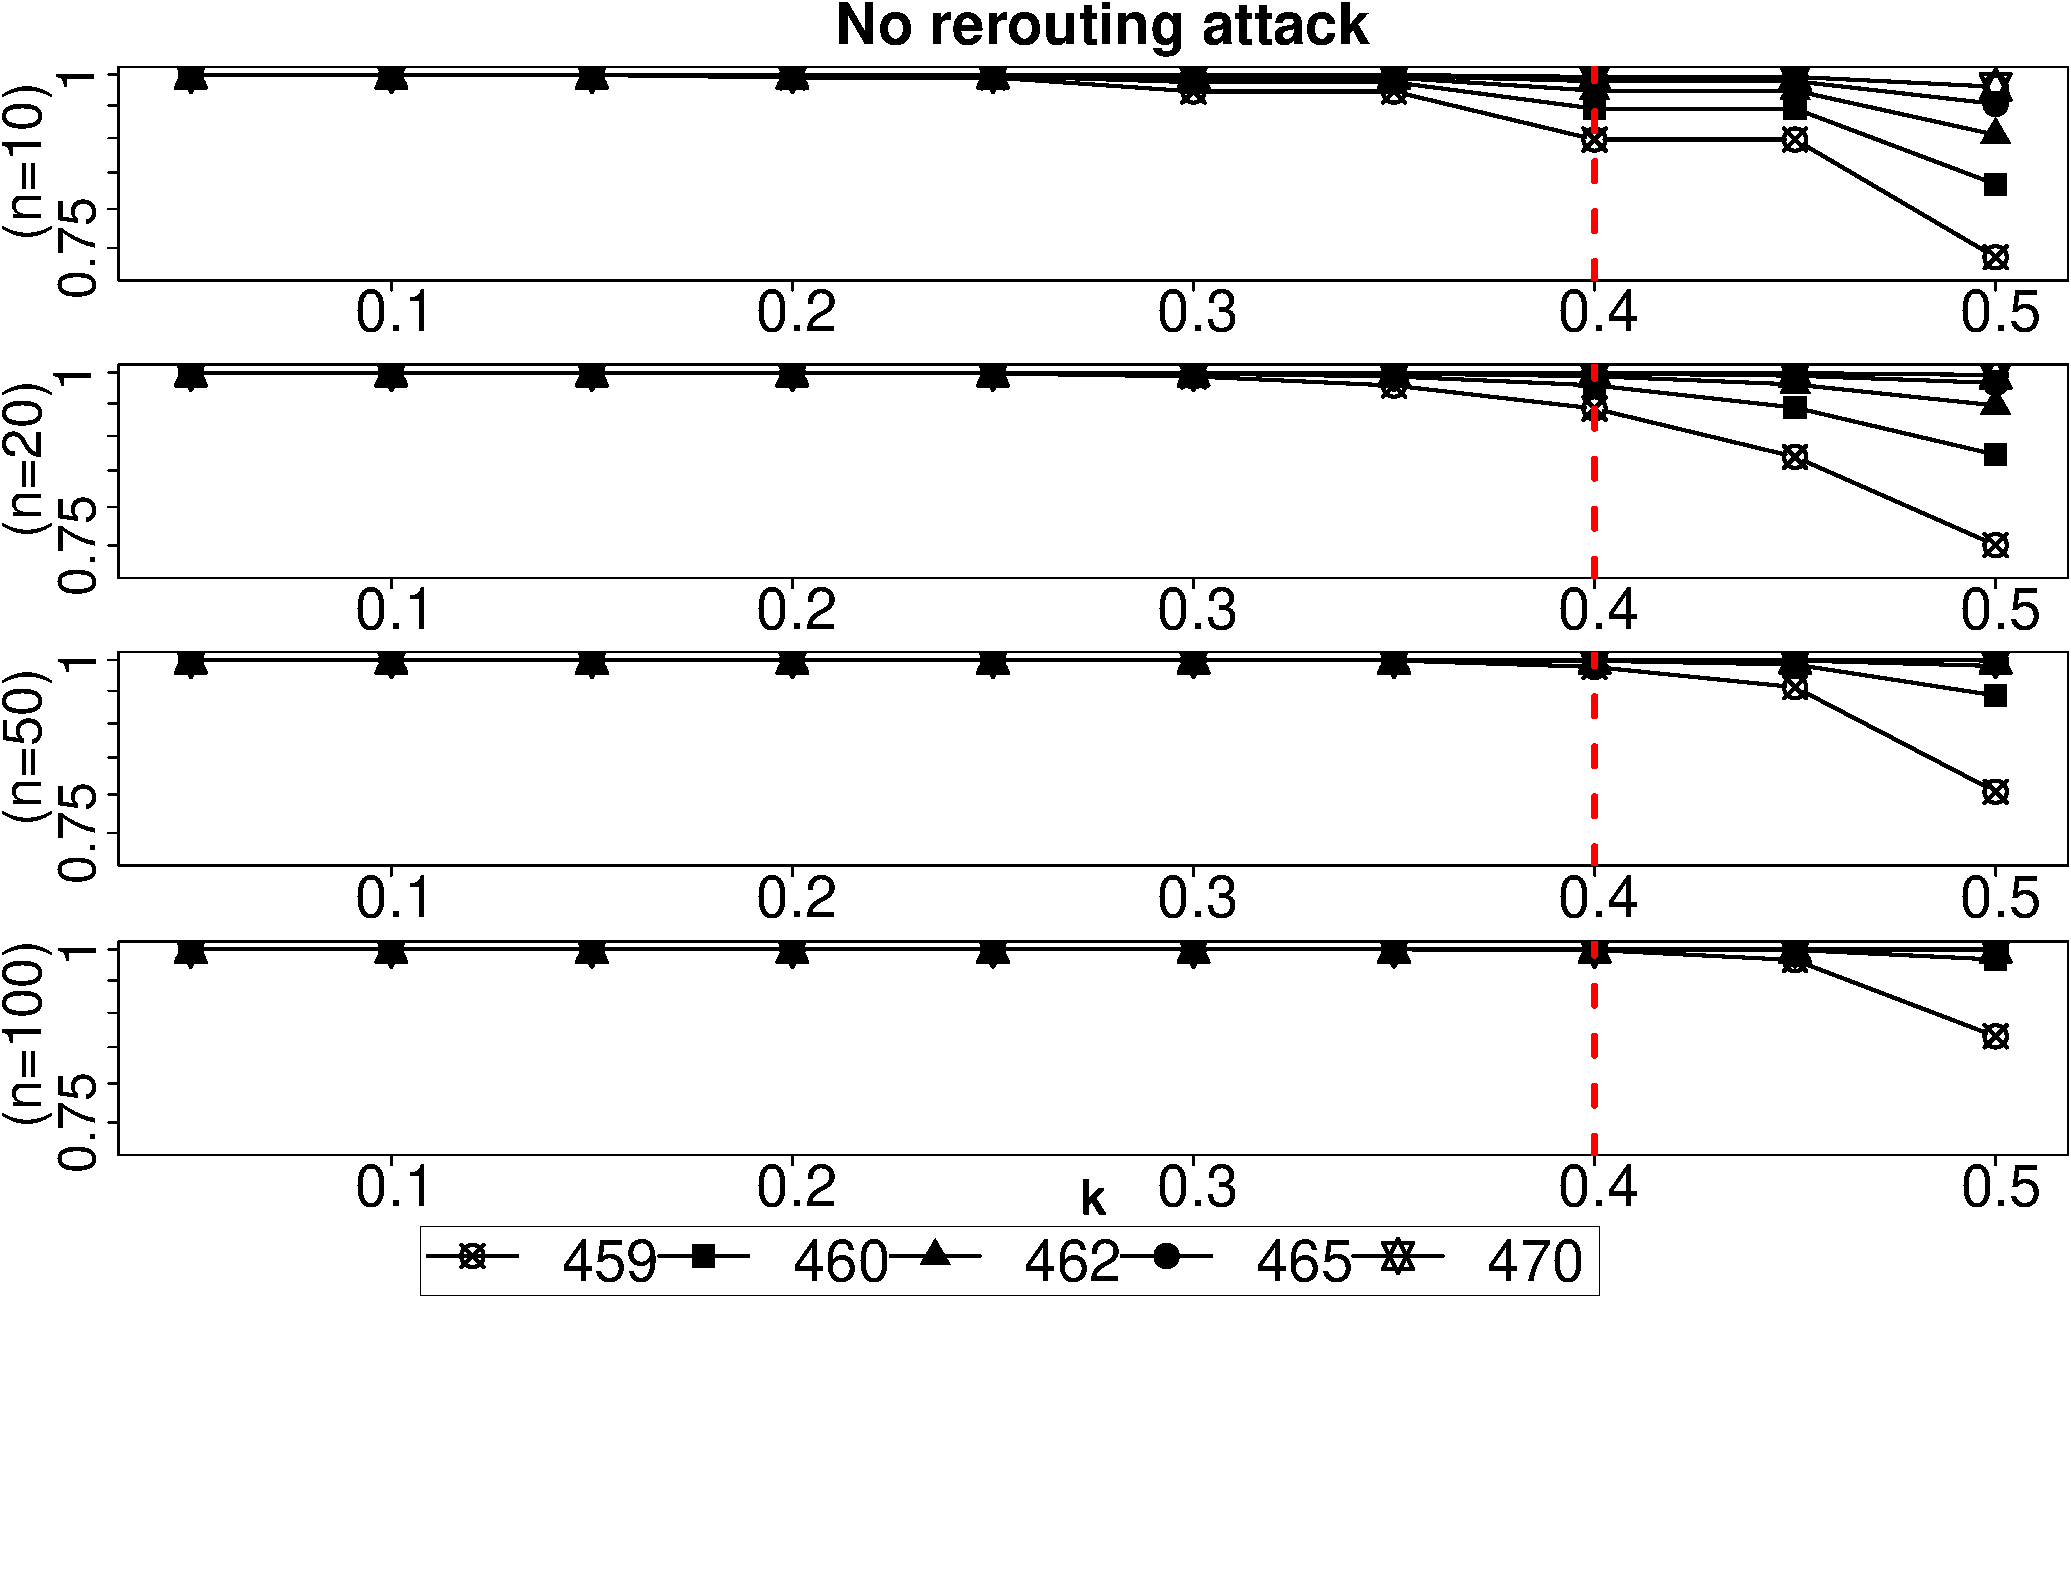
\includegraphics[trim={0 5cm 0 0}, clip, width=\linewidth]{data/graph/timeRound_new.pdf}
        \caption{\timeRoundCaption}
        \label{graph:diffTh}
    \end{subfigure}%
    ~ ~~
    \begin{subfigure}[t]{0.33\textwidth}
        \centering
        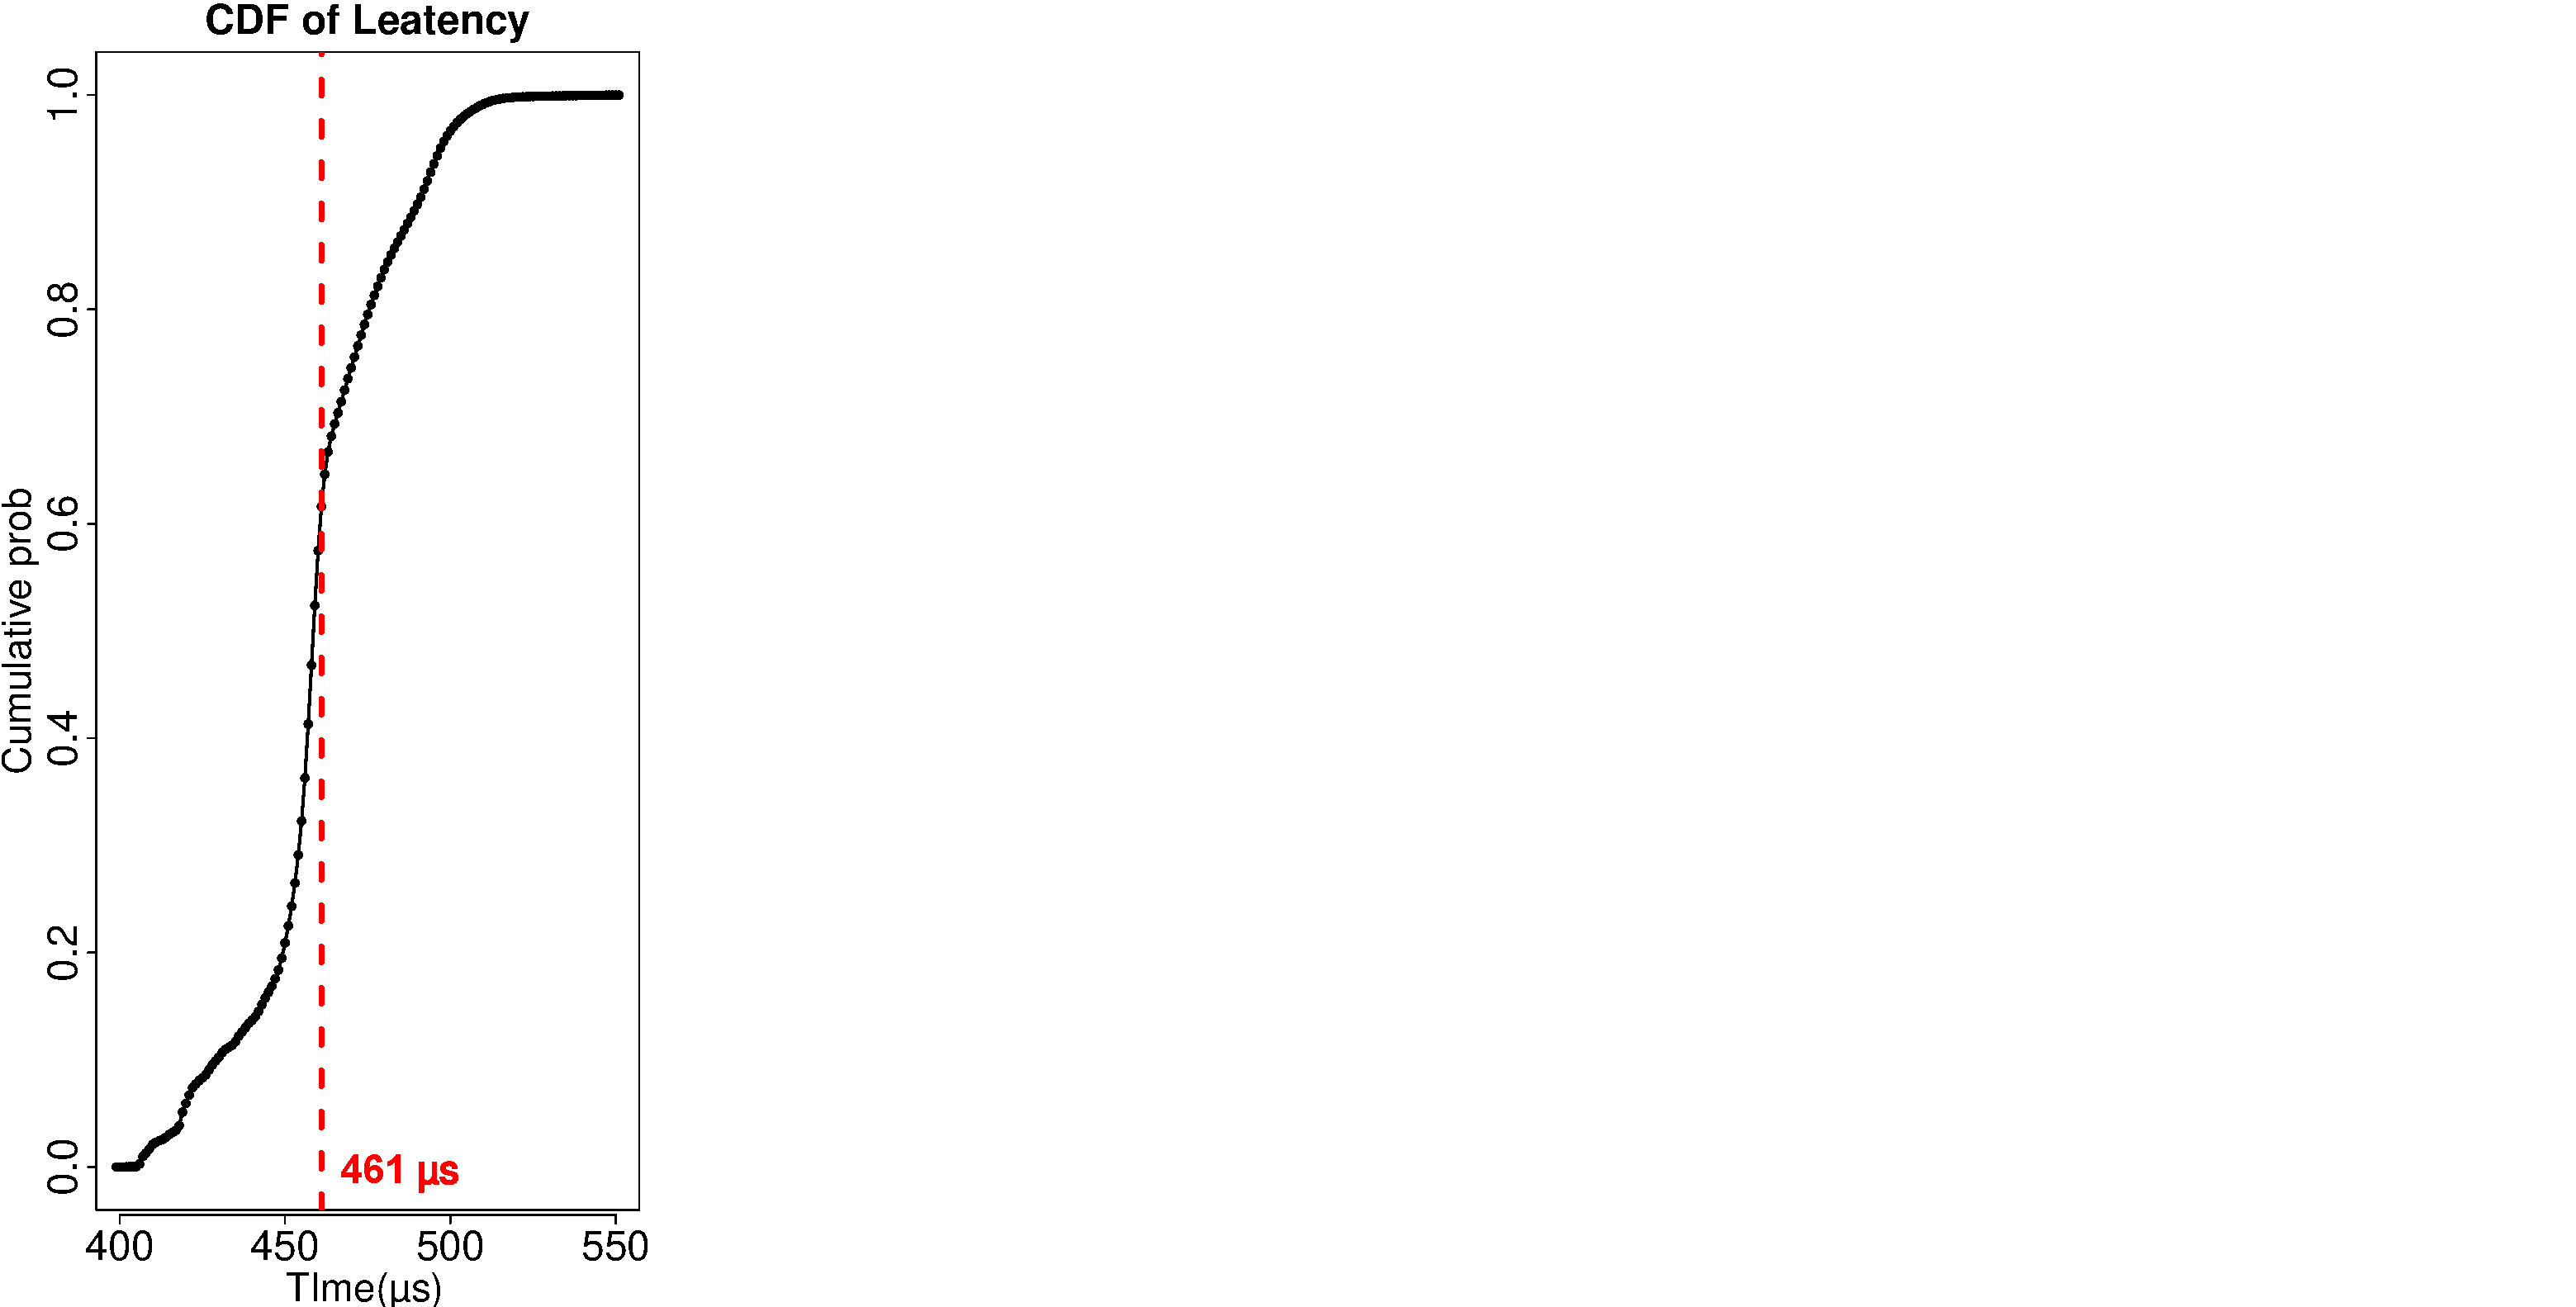
\includegraphics[trim={-0.6in 0cm 24cm 0}, clip, height=2.7in]{data/graph/CDF_Latency2.pdf}
        \caption{\cumulativeCaption}
        \label{fig:cdf}
    \end{subfigure}
    \caption{\textbf{Setting up threshold time (\connect) for \name.}}
\end{figure*}

\fi


\ifusenix
\vspace{-10pt}
\else
\fi
\myparagraph{Finding suitable threshold \connect.} Finding a suitable latency threshold \connect is a non-trivial task. A low threshold requires a high number of the challenge-response rounds, since the protocol (cf.\ Section~\ref{sec:ourApproach}) requires at least a fraction $k$ of the observed responses to be less or equal to \connect and the lower threshold has very low cumulative probability value in the latency distribution (see Figure~\ref{graph:reroutingDetectionHist}).
Conversely, a high threshold value enables some latencies measured during an attack to be classified as legitimate local replies, hence increasing the chances of the attacker to break the proximity verification. To address this challenge, we perform a trial over multiple threshold candidates to evaluate their viability.
%falls into the probability distribution of the case where the attack takes place, allowing the attacker to have a higher chance to break proximity verification.

Figure~\ref{graph:diffTh} shows the legitimate success probability $P_{legit}$ for different number of rounds ($n\in\{10,20,50,100\}$). We iterate through multiple threshold times (\connect$\in\{459\mu s,460\mu s,462\mu s,465\mu s,470\mu s\}$), and $470\mu s$ provides high success ratio for different values of $k$ ($P_{legit}=0.9\{7\}65$\footnote{$0.9\{n\}x$ denotes $0.n$-times $9$ followed by $x$.} $(n=50)$ and $P_{legit}=0.9\{13\}71\ (n=100)$).
%
We chose to test \connect up until $470 \mu s$ because as can be observed in figure~\ref{graph:reroutingDetectionHist} for these values we observe extremely small occurrences ($9.73\times10^{-2}$) of latency responses during an attacking scenario. It is possible to increment the latency further to improve the success probability, but doing so will start increasing the probability for the attacker as well. 
%
After that, we estimate that any latency value less than or equals to the threshold \connect appears with the cumulative probability of $p_c = \Pr[396\leq x \leq 470] = \sum_{i=396}^{470}\Pr[x=i] = 0.75$ (where $396\ \mu s$ is the smallest latency experienced).
%
\iffalse
%this is no longer necessary
Using the standard error of the mean, we estimated the error in our model, which is approximately $p_e=1/(2\sqrt{\mathcal{N}})$~\footnote{Hoeffding's inequality~\cite{Hoeffding} describes that one needs at least $\frac{log(2/\alpha)}{2t^2}$ samples to acquire $(1-\alpha)$-confidence interval $E(\bar{X})\pm t$, we set $1-\alpha=95\%$.} where $\mathcal{N}$ denotes the number of samples drawn in our experiment.
We have around $\mathcal{N}=27$ million samples to construct the distribution. This makes the sampling error probability $p_e \approx 1.06\times10^{-4}$.
%
The attacker's success probability $p_\mathcal{A}$ for a single round is simply the sampling error, i.e., $p_\mathcal{A} = p_e = 1.06\times10^{-4}$ due to the standard error of the mean as in our experiment we encounter zero samples within 461 $\mu s$ for attack distribution. The legitimate enclave's success probability $p_\mathcal{H}$ for a single round is the cumulative probability above, i.e.,  $p_\mathcal{H} = p_c = 0.6461$, as can be seen from Figure~\ref{fig:cdf}.
\fi

The attacker's success probability for a single round is the cumulative probability sampled from the attacker's distribution (the grey histogram in Figure~\ref{graph:reroutingDetectionHist}) $p_\mathcal{A} = \Pr[x \leq 470] = \sum_{i=451}^{470}\Pr[x=i] = 9.73 \times 10^{-5}$.


Now, for both cases (simulated attack and benign case) we can model the complete challenge-response protocol of $n$ rounds as a Bernoulli's trial where we look for at least $kn$ responses within $470\ \mu s$ out of $n$. We can write this cumulative probability as a binomial distribution:
%
%\vspace{-1px}
\ifusenix
\begin{align*}
    \Pr[x \geq nk] = \sum_{i=nk}^n\binom{n}{i} (p)^{i}(1-p)^{n-i};~~\text{where}~ p \in \{p_\mathcal{H}, p_\mathcal{A}\}
\end{align*}
%  \vspace{-3px}

\else
\begin{align*}
    \Pr[x \geq nk] = \sum_{i=nk}^n\binom{n}{i} (p)^{i}(1-p)^{n-i}
\end{align*}
%  \vspace{-3px}
where $p \in \{p_\mathcal{H}, p_\mathcal{A}\}$.
\fi

\ifusenix
\vspace{-10pt}
\else
\fi
\myparagraph{Choosing a suitable fraction $k$.} The next step of the evaluation is to find a suitable fraction $k$ based on the threshold time \connect. Note that both the success probability of the attacker and the legitimate enclave is calculated as the cumulative probability from a binomial distribution (from $nk$ to $n$). Hence, we require to choose a suitable value of $k$ that maximizes $P_{legit}$ while minimizing $P_{adv}$.

We calculate two graphs that are depicted in Figure~\ref{graph:roundSuccess} where the x-axis denotes $k$, and the y-axis denotes attacker's success probability $P_{adv}$ and legitimate success probability $P_{legit}$, respectively, while using \connect$=470 \mu s$. We observe a sharp decrease in the legitimate success probability at $k=0.4$. Hence, fix $k=0.4$ to achieve the maximum $P_{legit}$. Additionally, in the graph of attacker's success probability, the blue horizontal line is placed at $10^{-40} \approx 2^{-133}$. Hence we propose to choose any round configuration bellow this horizontal line, where $n \geq 25$. With number of rounds set to $n=50$ and $k=0.4$, we have $P_{legit}=0.999999965$ and $P_{adv}=2.71\times 10^{-67}$. Similar result could be also observed in Figure~\ref{graph:roundSuccess} where the success probability of the legitimate enclave decreases significantly after $k=0.55$ for \connect$=470\mu s$.

\newcommand{\roundCompCaption}{\textbf{Finding suitable fraction $k$.} The graph shows the legitimate enclave's success probability in an ideal scenario and the attacker's success probability in rerouting attack scenario with varying $k$.}
%The x-axis of the graph shows the threshold $k$ that denotes that at least $nk$ challenge-response out of $n$ has to be less or equal to $470\ \mu s$. 
%The blue line in the upper graph denotes negligible success probability ($10^{-40}\approx 2^{-133}$) for the attacker.}

\newcommand{\mainResultCaption}{\textbf{\name result in distinguishing rerouting attack.} The graph shows the attacker's success probability $P_{adv}$ and the legitimate success probability $P_{legit}$ in proximity verification for different number of rounds ($n$) given a fixed $k=0.4$.}% in the scenario where the attacker's average network latency is $153\ \mu s$ using the \texttt{ping} flood mode.}

\ifusenix
\begin{figure}[t]
  \centering
    %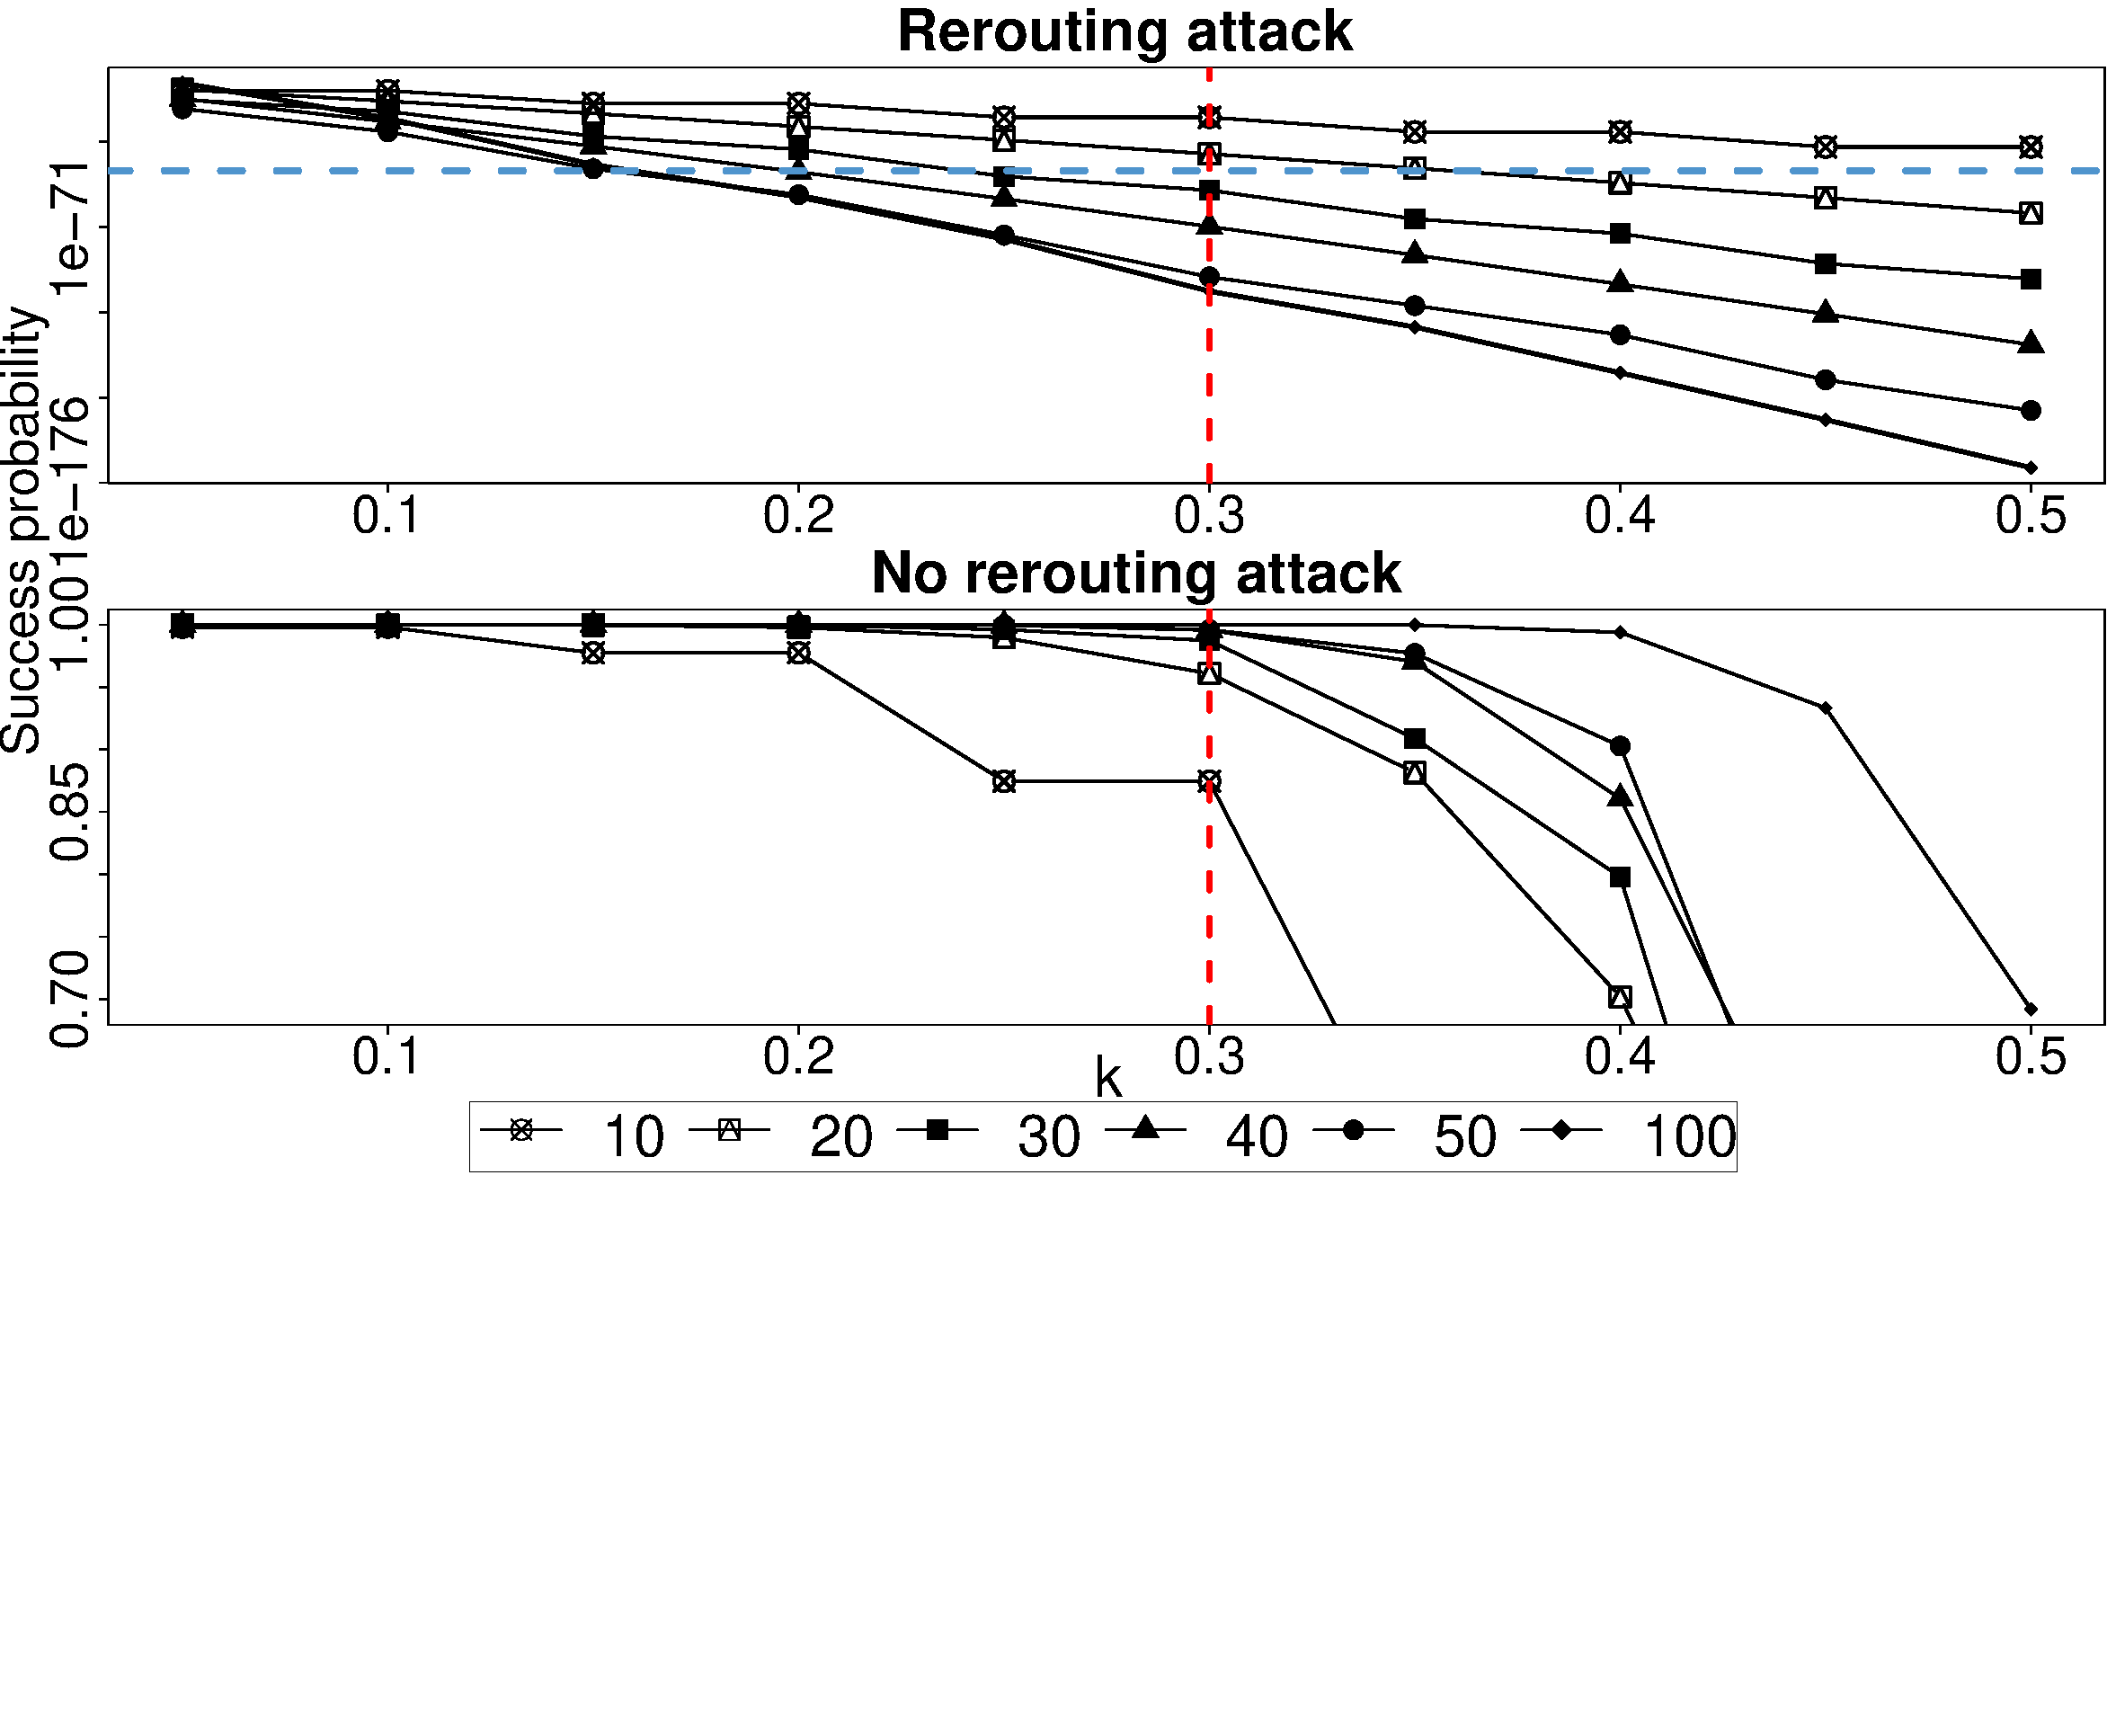
\includegraphics[trim={0 10.6cm 0 0}, clip, width=0.9\linewidth]{data/graph/round_comp_1.pdf}
    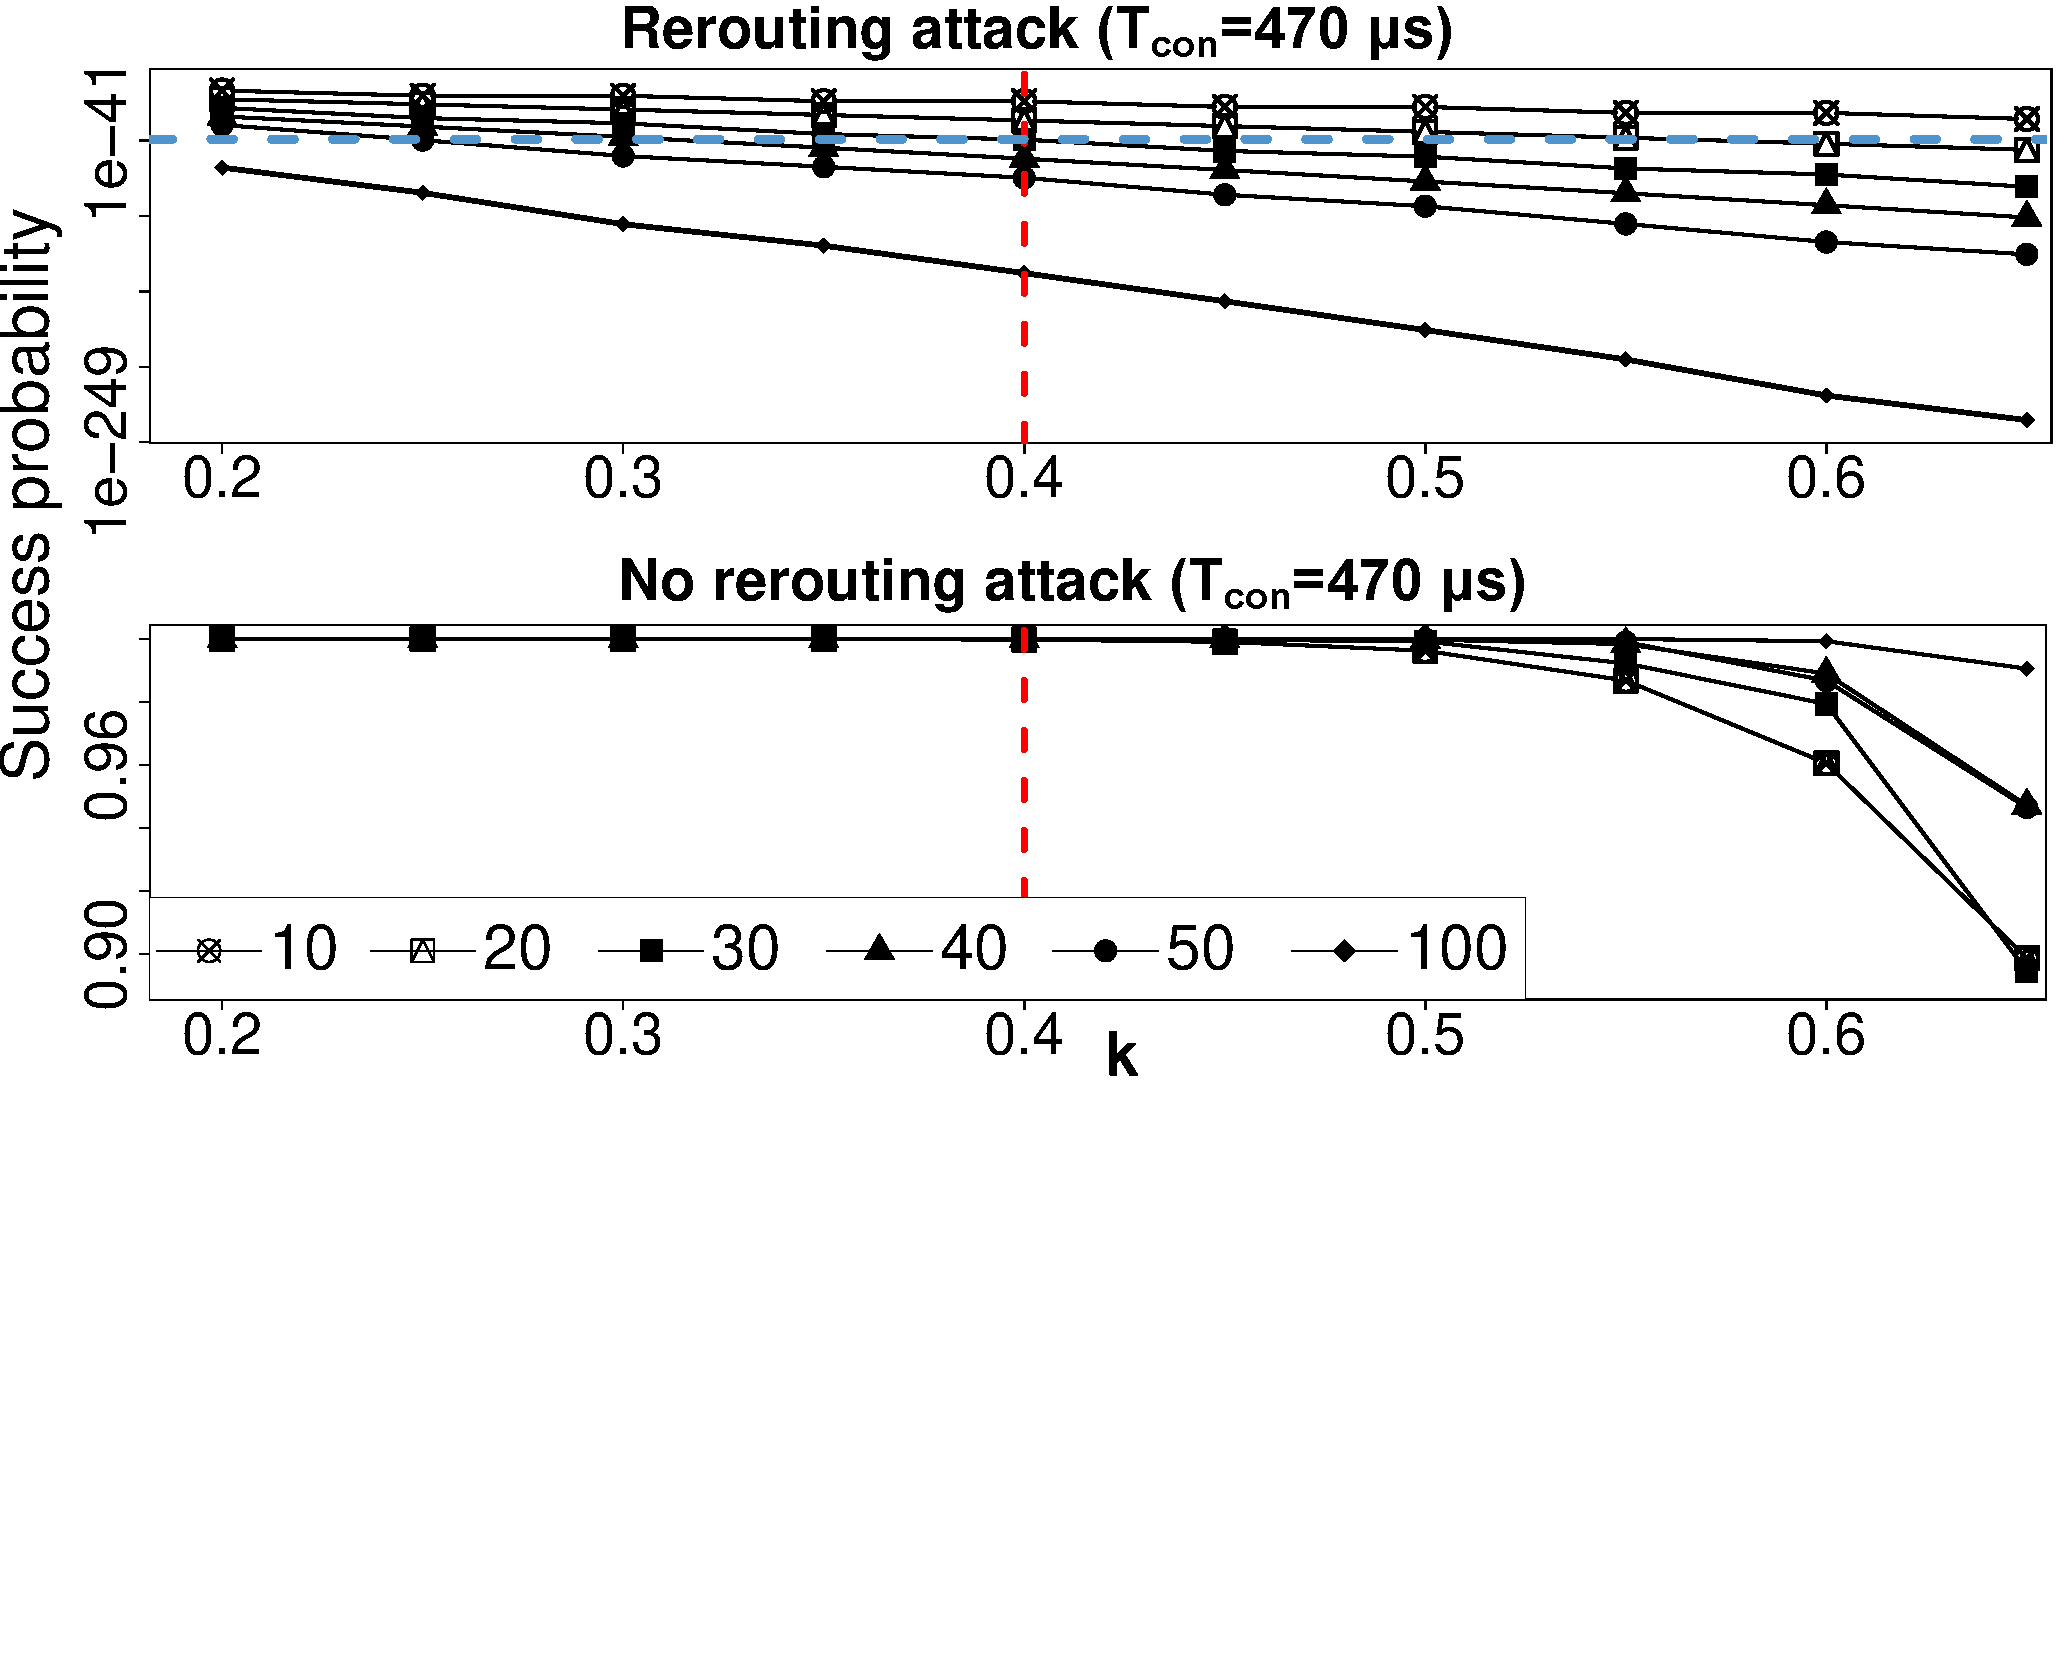
\includegraphics[trim={0 10cm 0 0}, clip, width=\linewidth]{data/graph/round_comp_new.pdf}
    \caption{\roundCompCaption}
    %\vspace{-5px}
    \label{graph:roundSuccess}
\end{figure}

\begin{figure}[t]
  \centering
    %\includegraphics[trim={0 1cm 0 0}, clip, width=0.9\linewidth]{data/graph/AttackerSuccess_combined.pdf}
    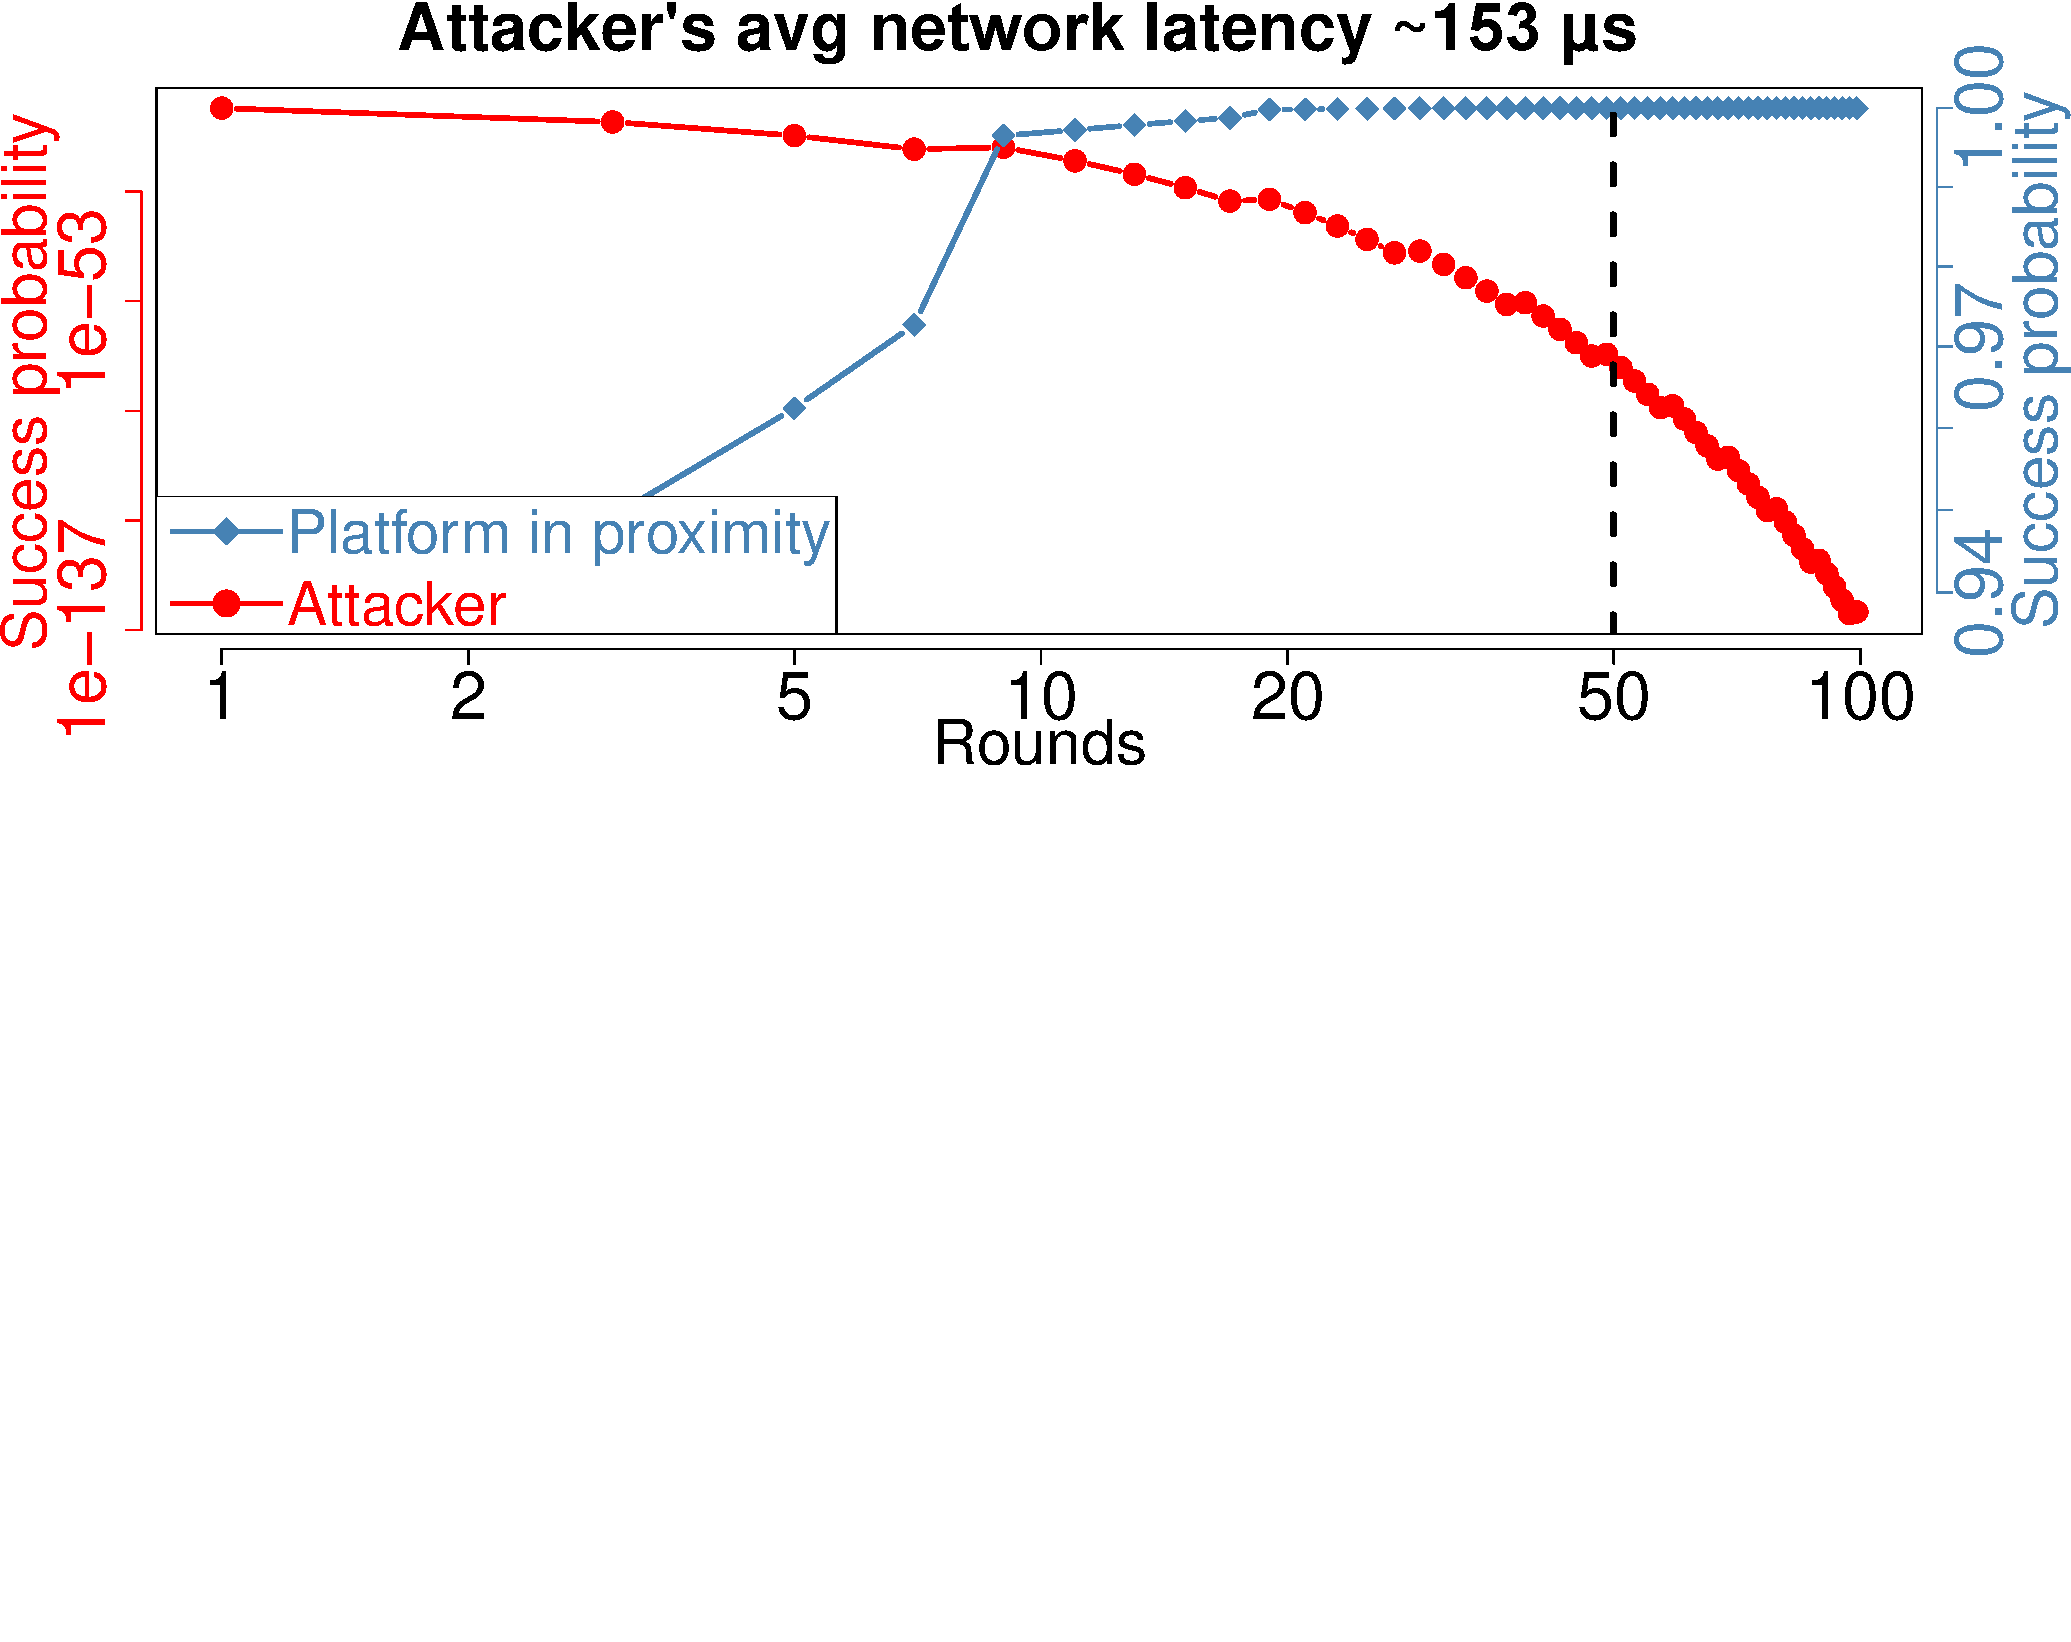
\includegraphics[trim={0 14.5cm 0 0}, clip, width=0.9\linewidth]{data/graph/AttackerSuccess_combined_new.pdf}
    %\includegraphics[trim={0 12.5cm 0 0}, clip, width=\linewidth]{data/graph/AttackerSuccess_colocated.pdf}
    \caption{\mainResultCaption}
   \vspace{-10px}
    \label{graph:attackerSuccess}
\end{figure}

\else

\begin{figure*}[t!]
    \centering
    \begin{subfigure}[t]{0.5\textwidth}
        \centering
        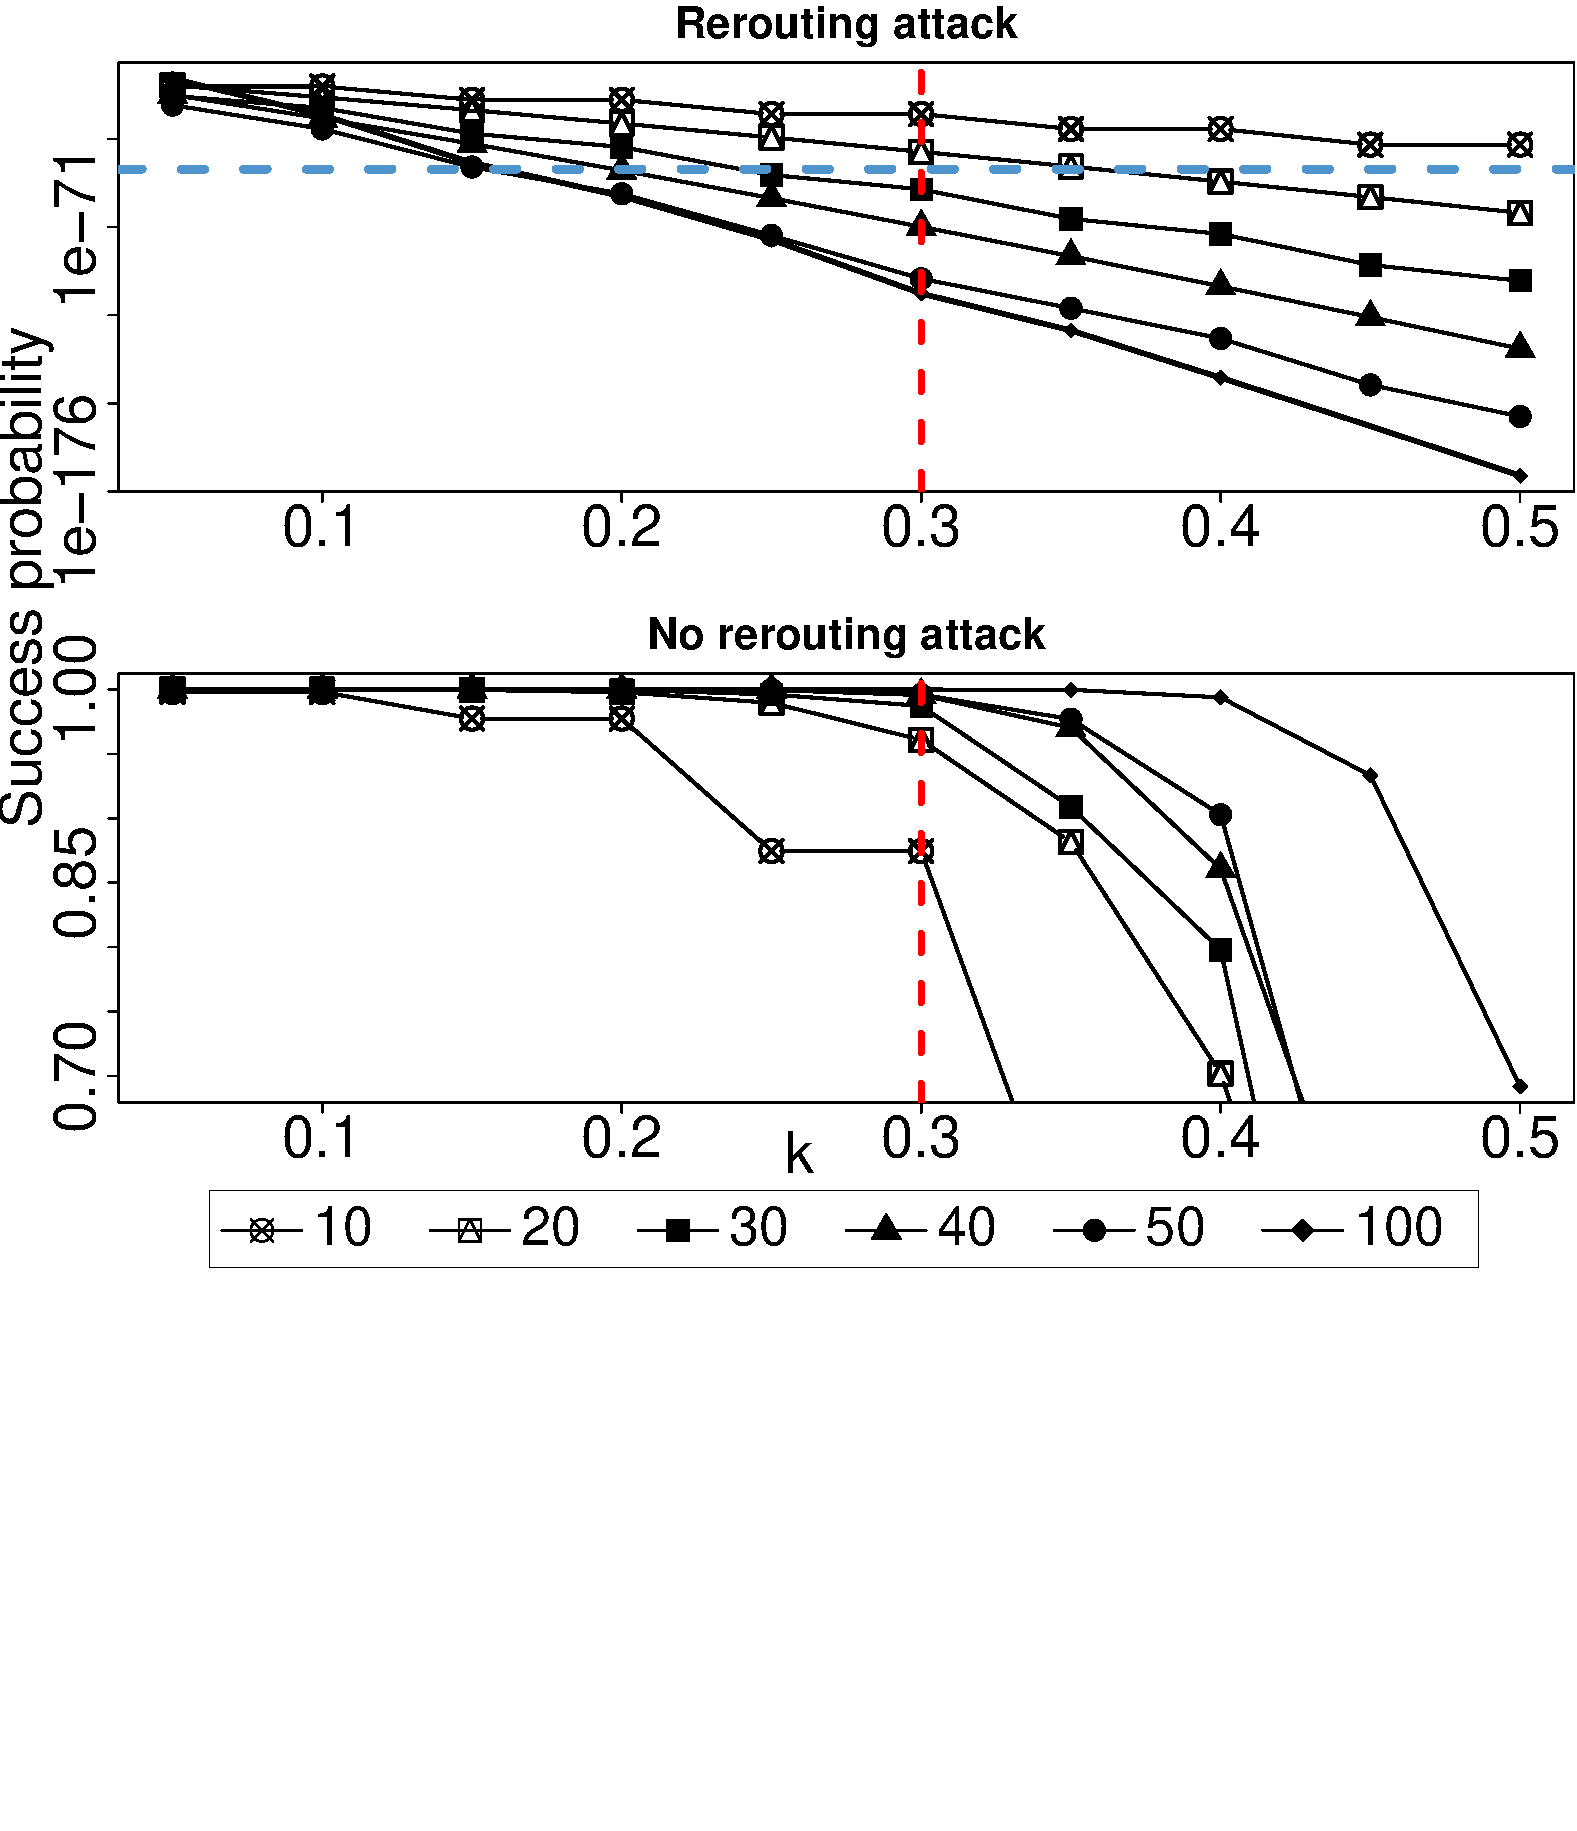
\includegraphics[trim={0 9.5cm 0 0}, clip,  height=2.2in]{data/graph/round_comp_2.pdf}
        \caption{\roundCompCaption}
        \label{graph:roundSuccess}
    \end{subfigure}%
    ~ ~~
    \begin{subfigure}[t]{0.5\textwidth}
        \centering
        \includegraphics[trim={0 0 0.5in 0}, clip, height=2.4in]{data/graph/AttackerSuccess_combined_1.pdf}
        \caption{\mainResultCaption}
        \label{graph:attackerSuccess}
    \end{subfigure}
    \caption{\textbf{Main experimental results of \name.}}
\end{figure*}
\fi
%
% \begin{figure}[t]
%   \centering
%     \includegraphics[trim={0 12.5cm 0 0}, clip, width=\linewidth]{data/graph/AttackerSuccess_colocated.pdf}
%     \caption{\textbf{Attacker's success and legitimate success in flood ping more.} This plots shows the attacker's success probability $P_{adv}$ and the legitimate success probability $P_{legit}$ in proximity verification for different number of rounds $n$ given a fixed fraction $k=0.3$ where the average ping latency is $103\mu s$.
%     \vspace{-20px}}
%     \label{graph:attackerSuccessClose}
% \end{figure}

\ifusenix
\vspace{-10pt}
\else
\fi
\myparagraph{Generalizing the number of rounds $n$.} Figure~\ref{graph:attackerSuccess} extends this analysis to the general number of challenge-response rounds spanning from $n=2$ to $100$ where the attacker uses \texttt{ping} in food mode and achieves $153\mu s$ average network latency. Here we compute the probability of attacker returning the reply within $470 \mu s$ for at least $k=0.4$ fraction of challenges. The y-axis denotes the attacker's success probability which diminishes overwhelmingly with the increasing number of challenges (keeping the fraction constant at $k=0.4$). Notice that, by merely choosing a higher number of rounds, satisfying values for the legitimate and attacker's success probabilities can be achieved even in the case in which the attacker manages to optimize the kernel for minimum network latency. Hence, \name can distinguish legitimate enclave and the attacker despite the lower latency. As long as the network latency is not negligible even smaller attacker's latencies than we could measure can be protected against by employing a higher number of challenge-response rounds.

\ifusenix
\vspace{-10pt}
\else
\fi
\myparagraph{Parameters for different settings.}
Note that in general, our ad hoc method for selecting the parameters involved in the protocol might not be optimal. An optimal solution is one that minimizes the number of rounds, to make the initial attestation faster, while having some lower bound constraint on $P_{legit}$ and an upper bound constraint on $P_{adv}$. Nevertheless, for the system that we tested, we were able to find satisfying values for the parameters, for instance, $50$ rounds can be performed in $~25 ms$.
It is important to observe that different systems might exhibit slightly different USB and network latencies. Therefore, if the reduction of the initial attestation time is a key requirement for the system in which \device is being deployed, a platform profiling step (essentially collecting the data presented in Figure~\ref{graph:reroutingDetectionHist} for the target system) might allow reducing further the time required for the initial attestation for a particular system.


\subsection{Periodic Proximity Verification Params}
\label{sec:evaluationL:continuousParameters}

%There are two primary parameters upon which we evaluate the security of periodic proximity verification. $P'_{adv}$ is the attacker's success probability where the attacker disconnects/reroutes the platform, and the \device continue to communicate. $P'_{adv}$ must be negligible for the security of \name. $P'_{fp}$ is the false positive probability where the \device disconnects the platform in proximity despite the legitimate enclave is running on that platform. $P'_{fp}$ negatively affects the availability of the system. Hence it should be low.

We set the periodic proximity verification parameters based on our experimental results following two main requirements. First, the attacker's success probability $P'_{adv}$ must be negligible. $P'_{adv}$ is identical to the false negative ($P'_{fn}$) as here \name rules out an attack even though an attack takes place. Second, the probability of false positives $P'_{fp}$ should be very low. Next, we explain the three-step process to set up the parameters: \detach, $w$ and $f$ for the periodic proximity verification. We refer to figure~\ref{fig:slidingWindow} in Section~\ref{sec:systemDesign} where we discussed the sliding window strategy for the continuous proximity verification. We proceed as follows:


\begin{mylist}
  \item We find out a suitable latency \detach that define the yellow or red round in Figure~\ref{fig:slidingWindow}. Yellow window define the round of challenge response latency between \connect and \detach, while the red window define a latency more than \detach. Hence, the probabilities $\Pr[T_{con}\leq \mathcal{L}_{legit}\leq T_{detach}]=\Pr[legit\in\text{yellow}]$, and $\Pr[\mathcal{L}_{legit} \geq T_{detach}]=\Pr[legit\in\text{red}]$ should be very low. $\mathcal{L}_{legit}$ and $\mathcal{L}_{A}$ denote the latency of the legitimate enclave running on the platform in proximity and remote attacker platform's latency respectively.
  \item Based on the threshold \detach, we select a suitable sliding window size $w$ to minimize the attacker success probability $P'_{adv}$ to a negligible quantity.
  \item We fix a suitable frequency $f$ for the periodic challenges. A high $f$ value terminate the communication very fast, leaving very small attacking window.
\end{mylist}

%We note that choosing parameter is different from the previous (Section~\ref{sec:evaluation:parameters}) as the continuous proximity verification executes in parallel to the data channel between the \device and the \app, we do not need to optimize the process for the size of the sliding window (which has the very similar to the number of rounds $n$).

\ifusenix
\vspace{-12pt}
\else
\fi
\myparagraph{Finding suitable threshold \detach.} We set the threshold \detach to $510\ \mu s$. We choose this value as we experience zero sample from the timing distribution (refer to the `yellow' distribution Figure~\ref{graph:reroutingDetectionHist}) where no rerouting attack takes place. While in the attacker's distribution, the cumulative probability of the response occurring between \connect and \detach is $Pr[$\connect$\leq \mathcal{L}_{A} \leq$\detach$]=\sum_{i=451}^{510}\Pr[\mathcal{L}_{A}=i]=1.4\times10^{-2}$. 
%We account for the experimental error in our model using the standard error of the mean as  $p_e \approx 1.06\times10^{-4}$. The value $p_e$ signifies that a legitimate enclave running on the platform in proximity may take more than 649 $\mu s$ to respond. 
Using \detach, we can now define the challenge response rounds in Figure~\ref{fig:slidingWindow} for a \emph{single round} as following:

\ifusenix
\vspace{-2pt}
\else
\fi
\begin{align*}
\Pr[\mathcal{L}_{legit}\leq T_{con}]&=\Pr[legit\in\text{green}]=0.75\\
\Pr[T_{con}< \mathcal{L}_{legit}< T_{detach}]&=\Pr[legit\in\text{yellow}]= 0.237\\
\Pr[\mathcal{L}_{legit}\geq T_{detach}]&=\Pr[legit\in\text{red}]= 7.09\times10^{-3}\\
\Pr[\mathcal{L}_{A}\leq T_{con}]&=\Pr[A\in\text{green}]=9.73\times10^{-5}\\
\Pr[T_{con}< \mathcal{L}_{A}< T_{detach}]&=\Pr[A\in\text{yellow}]= 1.4\times10^{-2}\\
\Pr[\mathcal{L}_{A}\geq T_{detach}]&=\Pr[A\in\text{red}]= 0.985\\
\end{align*} 
\ifusenix
\vspace{-20pt}
\else
\fi

\ifusenix
\vspace{-15pt}
\else
\fi
\myparagraph{Finding suitable sliding window size $w$.} Sliding window size is analogous to that of the number of rounds $n$. We keep  the size of the sliding window as $w=n=50$ as it only requires the \device to remember the past $50$ interactions and achieve high probability for the legitimate enclave and negligible success probability for the attacker. Similar to the previous approach, only if $20$ out of $50$ ($k=0.4$) challenge-response round where responses are within $470\ \mu s$, \name yields success probabilities as the following:

\ifusenix
\vspace{-4pt}
\else
\fi

\begin{align*}
 \Pr[A \in \text{success window}]&=P'_{adv} = P'_{fn}= 2.71\times 10^{-67}\\
 \Pr[A \in \text{failed window}]&=\Pr[A\in\text{red}]^2=0.970\\
 \Pr[legit \in \text{success window}]&=0.999999965\\
 \Pr[legit \in \text{failed window}]&=P'_{fp}=\Pr[legit\in\text{red}]^2=5\times10^{-5}
\end{align*}
\ifusenix
\vspace{-4pt}
\else
\fi

%leading to false negative (\name ruled out attack in a case of an attack) for the legitimate enclave of $3.77\times10^{-6}$) for the ideal scenario (refer to Figure~\ref{graph:roundSuccess}).


The probability that a halt window event occurs for a legitimate \app running on the platform in proximity is $\Pr[legit\in\text{red}]\approx 7.09\times10^{-3}$. The \device halts all the data communication to the target platform until the next periodic proximity verification.

If two or more than two latencies $\geq 510\mu s$ (\detach) are received, the \device terminates the connection and revoke the platform. The downtime that can happen as a result of false positive during a connection of 10 years is around $2$ minutes.

\ifusenix
\vspace{-25pt}.
\else
\fi
\myparagraph{Finding suitable frequency $f$.} The frequency $f$ determines how fast the connection is terminated in case the \device device is detached. Note that the \device takes around $12$ $ms$ on average to issue a new random challenge (by reading out the noise of the analog pins of the Arduino board) in the legitimate case. Hence, by performing a round of the protocol as soon as the previous is over, we achieve the maximum attainable average frequency of $\sim83$ rounds per second. We use this frequency as it consumes only $6.48$ KB (0.0011\% of the 
channel capacity) and allows the communication channel to be halted on average after $12 ms$ of the start of a relay attack and terminated in $24 ms$.

%\subsection{Faster Transfer Technologies}
%
%Here we discuss the practicality of \name that could be implemented on industry-standard data transfer technologies.
%
%\myparagraph{Faster \usb 3.0.} In the current prototype implementation of \device, we use an Arduino Duo (with native \usb 2.0) board which is a microcontroller based prototyping platform that provides established set of libraries and ease of usage. Note, that such prototyping platforms are not optimized for performance-oriented applications. One can easily implement on top of commercially available ARM processor-based \usb 3.0 prototyping board such as EZ-USB FX3~\cite{cyprass} board. The fundamental protocol level difference between \usb 2.0 and 3.0~\footnote{The \usb 2.0 uses polling based multiplex connection where the polling rate is around $125\mu s$ and the \usb 3.0 operates in much efficient peer to peer communication resulting in an order of magnitude wider bandwidth ($5$Gbit/s vs. $480$Mbit/s) and lower latency.} allows the EZ-USB FX3 to achieve around $5 \mu s$ round trip time compared to the $300 \mu s$ round trip time with the Arduino's \usb 2.0 controller.
%
%
%\myparagraph{Faster network interface.} One argument against \name could be the cloud provider may have an infrastructure based on the InfiniBand interface~\cite{infiniband} that provide microsecond level latency that could fool \name. We envision \name to be integrated with Thunderbolt 3 boards that can have direct memory access (DMA) and communicate over fast PCI Express. This provides faster response time compared to InfiniBand. We conclude that \name could ve viewed as a arms race between the latency of local and remote interfaces. As long as there exists a local transfer technology that is faster than the remote one, \name could distinguish a rerouting attack.

\subsection{Performance}

Finally, we evaluate our prototype's performance based on the following metrics.

\begin{mylist}
  \item \textbf{Start up latency.} The start-up latency of the \device is less than 1 second (to establish a \tls channel and execute the distancy-bounding protocol). The initial proximity verification takes 25 ms in the case of Variant I.
  %\todo{Can we be more precise here? How long does the distance bounding take in Variant I? What is the delay caused by the fact that communication goes through \device.}
  %This is the latency when the user starts the enclave for the first time alongside the \device. The startup phase includes the establishment of the \tls channel between the \device and the \app, executing the remote attestation process and executing the \name protocol.

  \item \textbf{Operational latency and data overhead.} The operation latency is defined as the additional latency our solution adds to normal communication from the remote verifier to the attested enclave. The operational latency is also minimal. Our solution adds around $200 \mu s$ for \tls and transport over the native \usb interface of the Arduino.
  The data overhead is around 80 bytes per packet for the header and the MAC. Execution of the periodic \name protocol with $83$ rounds/second only requires around $6.48$ KBytes/s of data which is only 0.0011\% of the \usb 2.0 channel capacity. Note that our implementation of the \device uses an \usb 2.0 connection, one can implement the \device on \usb 3.0 based platform to gain more performance.

  %\item \textbf{Continuous proximity verification.} Execution of the \name protocol with $20$ rounds only requires around $1.25$ KBytes of data. The continuous proximity verification is executed in parallel to the data channel between the \device and the \app, causing additional overhead to the trusted path. This protocol can be executed every second any costs only $4.5$ MBytes of data. As this \device never communicates these data over the network, it does not cause any network data overhead.

\end{mylist}
